\documentclass{article}
\usepackage{amsmath}
\usepackage{amssymb}
\usepackage{amsfonts}
\usepackage{epsfig}
\usepackage{theorem}
\usepackage{longtable}

\usepackage{url}
\usepackage{moreverb}
\usepackage{fancyhdr}
\usepackage{geometry}
\usepackage{times}
\usepackage{titlesec}
\usepackage{ragged2e}
\usepackage{graphicx}
\usepackage{xcolor}
\usepackage{comment}

% % % % % % % % % % % % % % % % % % % % % % % % % % % % % % % % % % % % 
\usepackage[normalem]{ulem} % For \sout
\usepackage[ruled]{algorithm2e}

% % % % % % % % % % % % % % % % % % % % % % % % % % % % % % % % % % % %

\usepackage{hyperref}
\usepackage{xspace}
\usepackage{cite}
\usepackage{framed}
\usepackage{algpseudocode} 
\usepackage{longtable}
\usepackage[capitalise,nameinlink,noabbrev]{cleveref}
\usepackage{url}
\usepackage{etoolbox}
\usepackage{fullwidth}

\newbool{showcomments}
\booltrue{showcomments}% comment this to hide comments




%============================



\DeclareMathOperator*{\argmin}{arg\,min}
\DeclareMathOperator*{\argmax}{arg\,max}

\DeclareMathOperator*{\arginf}{arg\,inf}
\DeclareMathOperator*{\argsup}{arg\,sup}

% \newcommand{\symboldefinition}[4]{#1}


\newcommand{\ehuffo}{{\epsilon_{\textrm{huff, 1}}}}
\newcommand{\ehufft}{{\epsilon_{\textrm{huff, 2}}}}
\newcommand{\mhufft}{{M_{\textrm{huff, 2}}}}



\newcommand{\activeconstraintsk}{{\mathbb A_{k}}}
\newcommand{\activeconstraintsl}{{\mathbb A_{l}}}
\newcommand{\activeconstraintskpo}{{\mathbb A_{k+1}}}

\newcommand{\atr}{A^{\infty}}
\newcommand{\btr}{b^{\infty}}

\newcommand{\bpr}{{B_{\infty}\left(p, r\right)}}
\newcommand{\bs}{{\beta^{(\star, k)}}}
\newcommand{\bsk}{{\beta_0^{(\star, k)}}}
\newcommand{\capcones}{{C^{(k)}_{\cap}}}
\newcommand{\capconeskmo}{{C^{(k-1)}_{\cap}}}
\newcommand{\chik}{{\chi_m^{(k)}}}
\newcommand{\chil}{{\chi_m^{(l)}}}
\newcommand{\ck}{c^{(k)}}
\newcommand{\ckpo}{{c^{(k+1)}}}
\newcommand{\dacc}{{\Delta_{\textrm{acc}}}}
\newcommand{\dacco}{{\Delta_{\textrm{a}}}}
\newcommand{\deltalargzik}{{\Delta_{\alpha,\beta}}}
\newcommand{\dfeas}{{\Delta_{\textrm{feasible}}}}
\newcommand{\dk}{\Delta_k}
\newcommand{\dl}{\Delta_l}
\newcommand{\dkpo}{\Delta_{k+1}}
\newcommand{\dsr}{{\Delta_{\textrm{sr}}}}
\newcommand{\fcki}{{C^{(k+1)}_{\textrm{in}}}}
\newcommand{\feasiblek}{{\mathcal F_m^{(k)}}}
\newcommand{\feasiblekmo}{{\mathcal F_m^{(k-1)}}}
\newcommand{\feasiblel}{{\mathcal F_m^{(l)}}}
\newcommand{\feasible}{{\mathcal F}}
\newcommand{\fmin}{f_{\text{min}}}
\newcommand{\gammabi}{\gamma_{\textrm{suff}}}
\newcommand{\gammasm}{\gamma_{\textrm{min}}}
\newcommand{\gcik}{{\nabla c_i \left(\xk\right)}}
\newcommand{\gk}{{\nabla m_f^{(k)}\left(\xk\right)}}
\newcommand{\gl}{{\nabla m_f^{(l)}\left(\xl\right)}}
\newcommand{\gmcik}{{\nabla m_{c_i}^{(k)}\left(\xk\right)}}
\newcommand{\gmcikmo}{{\nabla m_{c_i}^{(k-1)}\left(\xk\right)}}  
\newcommand{\gmcil}{{\nabla m_{c_i}^{(l)}\left(\xl\right)}}
\newcommand{\gradf}{\nabla f}
\newcommand{\hgik}{{\frac{\nabla m^{(k)}_{c_i}(\xk)}{\|\nabla m^{(k)}_{c_i}\left(\xk\right)\|}}}
\newcommand{\hk}{{\nabla^2m_f^{(k)}\left(\xk\right)}}
\newcommand{\huff}{{\Gamma_0}}
\newcommand{\huk}{{{\hat u}^{(k)}}}
\newcommand{\lipgrad}{{L_{\nabla}}}
\newcommand{\liphess}{{L_{\nabla^2}}}
\newcommand{\maxgrad}{{M_{\nabla}}}
\newcommand{\maxhessian}{{M_{\nabla^2}}}
\newcommand{\maxmodelhessian}{{M_{\nabla^2 m}}}
\newcommand{\maxnorm}{{M_{\|\cdot\|}}}
\newcommand{\mcik}{{{m}^{(k)}_{c_i}}}
\newcommand{\mcikmo}{{{m}^{(k-1)}_{c_i}}}
\newcommand{\mcil}{{{m}^{(l)}_{c_i}}}
\newcommand{\mck}{{{m}_{c}}^{(k)}}
\newcommand{\mf}{{{m}_f}}
\newcommand{\mfk}{{{m}_f}^{(k)}}
\newcommand{\mfkmo}{{{m}_f}^{(k-1)}}
\newcommand{\minactivegraddelta}{{\Delta_{\mathcal A}}}
\newcommand{\minactivegrad}{{ g_{\mathcal A} }}
\newcommand{\minanglealpha}{{ \alpha^{\star} }}
\newcommand{\minangledelta}{{\Delta_{\alpha^{\star}}}}
\newcommand{\mingraddelta}{{\Delta_{\nabla c}}}
\newcommand{\mingradepsilon}{{\epsilon_{\nabla c}}}
\newcommand{\mingrad}{{ g_{\textrm{low}} }}
\newcommand{\naturals}{\mathbb N}
\newcommand{\oalpha}{\tau_{\Delta}}
\newcommand{\omegadec}{\omega_{\text{dec}}}
\newcommand{\omegainc}{\omega_{\text{inc}}}
\newcommand{\outertrk}{{T_{\text{out}}^{(k)}}}
\newcommand{\outertrkpo}{{T_{\text{out}}^{(k+1)}}}
\newcommand{\polydn}{\mathcal{P}^d_n}
\newcommand{\qk}{{Q^{(k)}}}
\newcommand{\reals}{\mathbb R}
\newcommand{\rk}{\rho_k}
\newcommand{\Rm}{\mathbb R^m}
\newcommand{\Rn}{\mathbb R^n}
\newcommand{\rotk}{{R^{(k+1)}}}
\newcommand{\sampletrk}{{T_{\text{sample}}^{(k)}}}
\newcommand{\sampletrkpo}{{T_{\text{sample}}^{(k+1)}}}
\newcommand{\sampletrkmo}{{T_{\text{sample}}^{(k-1)}}}
\newcommand{\scaledunshiftedellipsoid}{{{\mathcal {\hat E}_{\text{feasible}}}^k}}
\newcommand{\sdk}{\delta_k}
\newcommand{\searchtrk}{{T_{\text{search}}^{(k)}}}
\newcommand{\sigmamax}{{\sigma_{\textrm{max}}}}
\newcommand{\sk}{{{s}^{(k)}}}
\newcommand{\thetamink}{{\pi^k_{\textrm{min}}}}
\newcommand{\tolcrit}{\tau_{\xi}}
\newcommand{\tolrad}{\tau_{\Delta}}
\newcommand{\trk}{\outertrk}
\newcommand{\trkpo}{\outertrkpo}
\newcommand{\trsinfset}{{E_\textrm{infeasible}}}
\newcommand{\trstol}{{\delta_\textrm{infeasible}}}
\newcommand{\unshiftedellipsoid}{{\mathcal E^k_{\textrm{feasible}}}}
\newcommand{\wik}{{w^{(i, k)}}}
\newcommand{\ximin}{\xi_{\text{min}}}
\newcommand{\xkpo}{{{x}^{(k+1)}}}
\newcommand{\xk}{x^{(k)}}
\newcommand{\xki}{x_i^{(k)}}
\newcommand{\xl}{{x^{(l)}}}
\newcommand{\xinit}{{x^{(0)}}}
\newcommand{\zik}{{z^{(i, k)}}}
\newcommand{\zil}{{z^{(i, l)}}}
\newcommand{\deltamingrad}{{\Delta_{\textrm{mm}}}}
\newcommand{\mingradmodel}{{ g_{\textrm{mm}} }}
\newcommand{\activefeasiblek}{{\mathcal F^{(k)}_A}}
\newcommand{\activechik}{{\chi_A^{(k)}}}
\newcommand{\qkmo}{{Q^{(k-1)}}}
\newcommand{\qkpo}{{Q^{(k+1)}}}
\newcommand{\ckmo}{{c^{(k-1)}}}
\newcommand{\sdkmo}{\delta_{k-1}}
\newcommand{\sdkpo}{{\delta_{k+1}}}
\newcommand{\projk}{{p^{(k)}}}
\newcommand{\projl}{{p^{(l)}}}
\newcommand{\projkl}{{p^{(k,l)}}}
\newcommand{\projlk}{{p^{(l,k)}}}
\newcommand{\projkk}{{p^{(k,k)}}}
\newcommand{\projll}{{p^{(l,l)}}}
\newcommand{\trueprojk}{{p_c^{(k)}}}
\newcommand{\truefeasiblek}{{F_c^{(k)}}}
\newcommand{\trueactiveprojk}{{\mathbb P_c^{(k)}}}
\newcommand{\nearlyactiveprojk}{{\mathbb P_{a}}}
\newcommand{\activeprojkk}{{\mathbb P^{(k, k)}}}
\newcommand{\activeprojkl}{{\mathbb P^{(k, l)}}}
\newcommand{\activeprojlk}{{\mathbb P^{(l, k)}}}
\newcommand{\activeprojll}{{\mathbb P^{(l, l)}}}
\newcommand{\unshiftedellipsoidpo}{{\mathcal E^{k+1}_{\textrm{feasible}}}}
\newcommand{\scaledunshiftedellipsoidpo}{{{\mathcal {\hat E}_{\text{feasible}}}^{k+1}}}
\newcommand{\unshiftedellipsoidkpo}{{\mathcal E^{k+1}_{\textrm{feasible}}}}
\newcommand{\image}{{\textrm{im}}}
\newcommand{\maxmodelgrad}{{M_{\nabla m}}}
\newcommand{\minangleu}{{replace me}}
\newcommand{\minanglediralt}{{w_f}}
\newcommand{\minangledir}{{u_{f not used anymore}}}
\newcommand{\minangledirk}{{u^{(k)}_f}}
\newcommand{\minangledirx}{{u_{f}(x_0)}}
\newcommand{\minangledirl}{{u^{(l)}_f}}
\newcommand{\epsactive}{{\mathbb A_c}}
\newcommand{\epsactivemodels}{{\mathbb A_{m}}}
\newcommand{\fik}{{C^{(i, k)}}}
\newcommand{\suffiterates}{{\mathcal K_{\textrm{suff}}}}
\newcommand{\miniterates}{{\mathcal K_{\textrm{min}}}}
\newcommand{\reduceiterates}{{\mathcal K_{\textrm{sr}}}}
\newcommand{\theircnot}{{\kappa_1}}
\newcommand{\theirc}{{\kappa_2}}
\newcommand{\zikthresh}{{ K_{\textrm{a}} }}
\newcommand{\jackk}{{J^{(k)}}}
\newcommand{\jackl}{{J^{(l)}}}
\newcommand{\jackkl}{{J^{(k)}_{\activeprojkk \cup \activeprojkl}}}
\newcommand{\jaclkl}{{J^{(l)}_{\activeprojkk \cup \activeprojkl}}}
\newcommand{\jackt}{{J^{(k)}_{\activeprojkk \cup \trueactiveprojk}}}
\newcommand{\huffeps}{{\epsilon_h}}
\newcommand{\huffalpha}{{\alpha_h}}
\newcommand{\huffdir}{{u_h}}
\newcommand{\huffdirk}{{u^{(k)}_h}}
\newcommand{\activeprojk}{{\textrm{active projection k}}}
\newcommand{\activeprojl}{{active projection l}}
\newcommand{\ulb}{{\mathcal U\left(\epsilon_{\textrm{lb}}\right)}}
\newcommand{\elb}{{\epsilon_{\textrm{lb}}}}
\newcommand{\slb}{{S_{\textrm{lb}}\left(\epsilon_{\textrm{lb}}\right)}}
\newcommand{\dlb}{{\Delta_{\textrm{lb}}\left(\epsilon_{\textrm{lb}}\right)}}


\newcommand{\convexdistance}{{D}}





\newcommand{\activeindicesk}{{ \mathbb I_h^{(k)} }}
\newcommand{\huffindicesk}{{ \mathbb H_h^{(k)} }}
\newcommand{\inactiveindicesk}{{ \mathbb J_h^{(k)} }}
\newcommand{\huffthreshold}{{\Delta_{\textrm{H}}}}


\newcommand{\deltalb}{{\delta_{\textrm{min}}}}


\newcommand{\minactivealpha}{{ \alpha_{\textrm{h}} }}
\newcommand{\activedirk}{{ u_{h}^{(k)} }}
\newcommand{\activegradmin}{{ g_{\textrm{h}} }}


\newcommand{\modeljack}{{ \nabla m^{(k)}_{c}\left(\xk\right) }}
\newcommand{\modeljacl}{{ \nabla m^{(l)}_{c}\left(\xl\right) }}
\newcommand{\truejack}{{ \nabla c\left(\xk\right) }}


\newcommand{\zmk}{{z_m^{(k, k)}}}
\newcommand{\zlk}{{z_l^{(k, l)}}}
\newcommand{\zck}{{z_c^{(k)}}}

\newcommand{\Amk}{{\mathbb A_m^{(k, k)}}}
\newcommand{\Alk}{{\mathbb A_l^{(k, l)}}}
\newcommand{\Ack}{{\mathbb A_c^{(k)}}}



% Added by Steve
\newcommand{\st}{\textrm{such that}}
\newcommand{\norm}[1]{{\left\|#1\right\|}}
\newcommand{\intr}{\operatorname{int}}





% Need to remove
\newcommand{\domain}{\Omega}
\newcommand{\dmax}{{\Delta_{\textrm{max}}}}
\newcommand{\ellipsek}{{E^{(k)}}}
\newcommand{\scaledellipsek}{{{\hat E}^{(k)}}}
\newcommand{\ak}{{\nabla m_c^{(k)}\left(\xk\right)}}
\newcommand{\bk}{{m_c^{(k)}\left(\xk\right)}}

\newcommand{\lca}{{A}}
\newcommand{\lcb}{{b}}
\newcommand{\lctra}{G^{(k)}}
\newcommand{\lctrb}{{g^{(k)}}}


\newcommand{\uk}{{\huk}}

\newcommand{\activei}{{\mathcal A}}
\newcommand{\alphaone}{{u_{\textrm{feasible}}}}
\newcommand{\alphatwo}{{\pi_1}}
\newcommand{\alphathree}{\pi_2}
\newcommand{\alphak}{\pi^{(k)}}
\newcommand{\alphakp}{\pi_3^{(k)}}
\newcommand{\unshiftedcone}{{C^{(k)}_{\textrm{unsh}}}}
\newcommand{\shiftedcone}{{C^{(k)}_{\textrm{sh}}}}
\newcommand{\deltaf}{\delta_{f}}


\newcommand{\condition}{{\kappa}}
\newcommand{\polyk}{{{\mathcal{P}}^{(k)}}}
\newcommand{\tolsr}{{\tau_{\textrm{ef}}}}
\newcommand{\slin}{{{\hat s}^{(k)}}}

\newcommand{\proj}{{\textrm{Proj}}}



\newcommand{\hullpoly}{\mathcal P_{\textrm{hull}}}
\newcommand{\dgood}{\Delta_{\textrm{fsr}}}



\newcommand{\nocontentsline}[3]{}
\newcommand{\tocless}[2]{\bgroup\let\addcontentsline=\nocontentsline#1{#2}\egroup}



%
% File thesis_environment.tex
%
% Description:
% This file contains environments for theorems, lemmas, definitions,
% proofs, corollaries, algorithms, examples, remarks, and assumptions.
% The numbering is set up so that the same counter is used for ALL
% these environments.  This seems to make it easier for readers to
% find referenced material.  The counter is reset for each chapter.
%
% EXAMPLE
%    Definition 3.1
%    Lemma 3.2
%    Example 3.3
%    Theorem 3.4
%    Theorem 3.5
%    Lemma 3.6 ....
%
%    Lemma 4.1
%    Corollary 4.2 ....
%
% The Definition environment is indented on both sides.  This
% is not required, but seemed to be a nice way to separate definitions
% from proven results.
%
%%%%%%%%%%%%%%%%%%%%%%%%%%%%%%%%%%%%



%============================

\newtheorem{theorem}{Theorem}[chapter]
\newtheorem{corollary}[theorem]{Corollary}
\newtheorem{definition}[theorem]{Definition}
\newtheorem{lemma}[theorem]{Lemma}

% \numberwithin{thoerem}{chapter}



\crefname{equation}{}{equations}

\newcounter{assumptioncounter}
\newenvironment{assumption}[1][]{\refstepcounter{assumptioncounter}\par\medskip
\textbf{Assumption \theassumptioncounter} \rmfamily \itshape}{\medskip}

\numberwithin{assumptioncounter}{chapter}
\crefname{assumptioncounter}{Assumption}{assumption}


\newenvironment{comment}
	{
		\ifbool{showcomments}{
			\par\medskip
			\color{red}%
			\begin{framed}
			\textbf{Comment: }
			\ignorespaces
		}{}
	}
	{
		\ifbool{showcomments}{
			\end{framed}
			\medskip
		}{}
	}


\def\proof{\par{\it Proof}. \ignorespaces}

\def\endproof{\vbox{\hrule height0.6pt\hbox{%
   \vrule height1.3ex width0.6pt\hskip0.8ex
   \vrule width0.6pt}\hrule height0.6pt
  }}

  
  
% \newcommand{\new}[1]{{\color{blue}#1}}
% \newcommand\hcancel[2][black]{\setbox0=\hbox{$#2$}\rlap{\raisebox{.45\ht0}{\textcolor{#1} {\rule{\wd0}{1pt}}}}#2} 
% \newcommand{\replace}[2]{{\color{red}\sout{#1}\color{black}{\color{red}#2\color{black}}}} %TeX source markup.
% \newcommand{\replaceb}[2]{{\color{blue}\sout{#1}\color{black}{\color{blue}#2\color{black}}}} %TeX source markup.
% \newcommand{\replacemath}[2]{{\hcancel[red]{#1}{}{\color{red}#2\color{black}}}} %TeX source markup.
% % \newcommand{\replacemath}[2]{{\color{red}#2\color{black}}} %TeX source markup.
% \newcommand{\replacemathb}[2]{{\hcancel[blue]{#1}{}{\color{blue}#2\color{black}}}} %TeX source markup.

\newcommand{\sbnote}[1]{
	\ifbool{showcomments}{
		\textsf{
			{
				\color{cyan}{ SCB note:}   #1
			}
		}
% 		\marginpar{
% 			{
% 				\textbf{Comment}
% 			}
% 		}
	}{}
}

% \newcommand{\sbnote}[1]{
% 		\textsf{
% 			{
% 				\color{cyan}{ SCB note:}   #1
% 			}
% 		}
% 		\marginpar{
% 			{
% 				\textbf{Comment}
% 			}
% 		}
% }

\newcommand{\outerfritr}{D_{\text{out}}}



\newcommand{\real}{\mathbb R}

\newcommand{\trialk}{{{s}^{(k)}}}
\newcommand{\matvec}{\mathrm{vec}}

\crefname{Lemma}{Lemma}{Lemma}
\crefname{Proposition}{Proposition}{Proposition}
\crefname{Corollary}{Corollary}{Corollary}
\renewcommand{\baselinestretch}{1.5}
%=========================================

\title{Model-Based Trust Region Methods for Derivative-Free Optimization with Unrelaxable Linear Constraints}
\author{Stephen C.  Billups and Trever Hallock}

\makeatletter
\def\BState{\State\hskip-\ALG@thistlm}
\makeatother

\let\oldref\ref
\renewcommand{\ref}[1]{(\oldref{#1})}
\def\INCLUDEOMITTED{0}
\begin{document}


\maketitle

\begin{abstract}
We propose a model-based trust-region algorithm for constrained optimization problems with linear constraints in which derivatives of the objective function are not available and the objective function values outside the feasible region are not available.
In each iteration, the objective function is approximated by an interpolation model, which is then minimized over a trust region.
To ensure feasibility of all sample points and iterates, we consider two trust region strategies in which the trust regions are contained in the feasible region.
Computational results are presented on a suite of test problems.

\end{abstract}
%
%\newpage
%
%\tableofcontents
%
%\newpage

\section{Introduction}
Derivative-free optimization (DFO) refers to mathematical programs involving functions for which derivative information is not explicitly available.
Such problems arise, for example, when the functions are evaluated by simulations or by laboratory experiments.
Applications of DFO appear in many fields, including photo-injector optimization \cite{Neveu2017},
circuitry arrangements \cite{PLOSKAS201816}, machine learning \cite{KS2018}, volume optimization \cite{Cheng2017}, and reliability-based optimization \cite{Gao2017}.
In such applications, function evaluations are typically expensive, 
so it is sensible to invest significant computational resources to minimize the number of function evaluations required.

This work is aimed at developing algorithms to solve constrained optimization problems of the form 
\begin{align}
\begin{array}{ccl} \min_{x \in \Rn} & f(x) \\
\mbox{subject to} \quad & c_i(x) \le 0, &\quad \forall 1 \le i \le m,
\end{array}
\label{the_dfo_problem}
\end{align}
where 
% $\domain$ is a subset of $\Rn$, and
$f$ and $c_i$ for $1 \le i \le m$ are real-valued functions on $\Rn$ with at least one of these functions being a {\em black-box} function, meaning that derivatives cannot be evaluated directly.
We let the feasible set be represented as
\begin{align}
\feasible = \{x \in \Rn \; | \; c_i(x) \le 0, \; \forall 1 \le i \le m \}.
\end{align}

We are interested in developing {\em model-based}, {\em trust-region} algorithms for solving these problems.
Model-based methods work by constructing model functions to approximate the black box functions at each iteration.
The model functions are determined by fitting previously evaluated function values on a set of sample points.
In trust-region methods, the model functions are used to define a trust-region subproblem whose solution determines the next iterate.
For example, the trust-region subproblem might have the form
\begin{align*}
\begin{array}{ccl} \min_{\|s\| \le \dk}
 & \mfk \left(\xk+s\right) \\
\mbox{subject to} \quad & \mcik\left(\xk + s\right) \le 0 & \quad 1 \le i \le m, \\
& \|s\| \le \dk \\
\end{array}
\end{align*}
where $\xk$ is the current iterate, $\mfk$ is the model function approximating $f$, 
and $\mcik$ are the model functions approximating the constraint functions $c_i, \forall 1 \le i \le m$, and $\dk$ is the radius of the trust-region.
The key differences between the trust-region subproblem problem and the original are that all functions are replaced with their model functions, 
and a trust region constraint ($\|s\| \le \dk$) has been added.

%Note that we are using models of the constraint functions to approximate the feasible region during each iteration.  In particular, we define the {\em model feasible region} by
%\begin{align}
%\feasiblek = \left\{x \in \Rn \big| \mcik(x) \le 0 \quad \forall 1 \le i \le m \right\}.  \label{define_feasiblek}
%\end{align}



Conceptually, the model functions are ``trusted'' only within a distance $ \dk $ of the current iterate $\xk$; 
so the trust-region subproblem restricts the length of step $s$ to be no larger than $\dk$.
To ensure that the model functions are good approximations of the true functions over the trust region, 
the sample points are typically chosen to lie within the trust-region.

We are specifically interested in applications where some of the black box functions cannot be evaluated outside the feasible region.  Constraints of this type can arise in several ways, such as when a simulation cannot be carried out on particular inputs.
For example, the authors of \cite{Padidar2021} optimize rapid-cycling synchroton lattice design,
but some overlapping synchrotron elements cannot be simulated.
Following the taxonomy in \cite{ledigabel2015taxonomy},  such constraints are called {\em unrelaxable}.

For problems involving unrelaxable constraints,  we require all iterates and sample points to be feasible.
As a first step toward developing algorithms to solve such problems, this paper considers a simplified problem where all of the constraints are linear and unrelaxable; namely:
\begin{align}
\begin{array}{ccl} \min_{x \in \Rn} & f(x) \\
& \lca x \le \lcb, & 
\end{array}
\label{linear_dfo_problem}
\end{align}
where $\lca$ is an $m \times n$ matrix and $\lcb \in \Rm$.
We assume that the rows of $A$ have been normalized so that $\|A_i\| = 1$.


An important consideration in fitting the model functions is the ``geometry'' of the sample set.
This will be discussed in more detail in \cref{geometry}, but the key point is that the relative positions of the sample points within the trust region have a significant effect on the accuracy of the model functions over the trust region.
When the geometry of the sample set is poor, it is sometimes necessary to evaluate the functions at new points within the trust region to improve the geometry of the sample set.
It is well understood how to do this for unconstrained problems, but for constrained problems
our requirement that the sample points must be feasible poses some interesting challenges to maintaining good geometry.   

In unconstrained optimization, it is natural for the sample trust region to be centered at the current iterate.
Thus, much of the standard theory (see for example, Chapter 3 of \cite{introduction_book})
of sample set geometry assumes the sample points are chosen within a ball centered at the current iterate.
However, for constrained problems,  this is no longer a useful assumption.
In particular, when iterates are close to the boundary of the feasible region, it is advantageous to shift the center of the sample trust region away from the current iterate.
Because of this, we rework some of the standard results to not require a sample point at the center of the sample trust region.


We propose an algorithm for solving \cref{linear_dfo_problem} whose main idea is to construct a feasible ellipsoid at each iteration that lies within the intersection of the feasible region and the current trust region.   We call this ellipsoid the {\em sample trust region}.
To choose well-poised sample points for this ellipsoidal region,  we adapt a model improvement algorithm presented in \cite{introduction_book} for spherical trust regions and establish error bounds on the accuracy of the model functions over this region.    

Convergence analysis is based on an algorithmic framework presented in \cite{Conejo:2013:GCT:2620806.2621814},  which describes a class of trust-region algorithms for convex constrained minimization without derivatives.   This framework assumes that a model of the objective function can be constructed at each iteration that satisfies certain accuracy assumptions, but it does not specify how to construct such a model function.    Here, we show that the model functions constructed by our algorithm satisfy these assumptions.  Hence,  using the results from \cite{Conejo:2013:GCT:2620806.2621814}, we show that
the criticality measure for the iterates generated by our algorithm converges to zero.  As a consequence, any accumulation point of the iterates satisfies the Karush-Kuhn-Tucker first order optimality conditions.  


\subsection{Notation}

Throughout the paper, superscripts are used to index members of a set or sequence, whereas subscripts denote components of a vector.  For example,  
$\xki$ is the $i$-th component of the $k$-th vector in the sequence $\{\xk\}$.
For a matrix $A$,  the $i$th row is denoted $A_i$, whereas the $j$th column is $A_{\cdot j}$.  
For a set of indices $S$,  $A_S$ is the submatrix formed by using only the rows of $A$ from the set $S$.   If $A$ is square, its condition number is $\condition(A)$, the smallest and largest eigenvalues are denoted 
$\lambda_{\text{min}}(A)$, and $\lambda_{\text{max}}(A)$, respectively.  $A \succ 0$ denotes that $A$ is positive definite.  

The projection of a point $x$ onto a convex set $X$ is denoted by $\proj_X(x) = \argmin_{x' \in X}\left\|x' - x\right\|$.  $B_p\left(c; \Delta\right)$ is the ball of radius $\Delta$ in the $p$-norm, centered at point $c$.  That is,  $B_p\left(c; \Delta\right) = \left\{x \in \Rn \bigg | \left\|x - c\right\|_p \le \Delta \right\}$.

When a norm is presented without a subscript, it is assumed to be the 2-norm.  For matrices, we will also use the Frobenius norm $\left\|\cdot\right\|_F$, defined by $\left\|A\right\|_F = \sqrt{\sum_i\sum_jA_{i, j}^2}$.

The complement of a set $S$ is denoted by $S^c$.   
Set addition is denoted by $X + Y = \left\{x + y | x \in X, y \in Y\right\}$, for subsets $X,Y \subseteq S$.

$\delta_{i,j}$ is the Kronecker delta, $\delta_{i, j} = \begin{cases} 1 & \textrm{if} \; i = j \\ 0 & \textrm{if} \; i \ne j \end{cases}$.
The positive part of a real number $a$ is denoted $a^+ = \max\{a,0\}$, whereas the $a^-=\max\{-a,0\}$.



\section{Background}
%\sbnote{I commented out the literature review for now.  We may not need to have a literature review section.}
%
%\sbnote{But, we should mention any papers that claim to deal with unrelaxable constraints.}

%\subsection{Literature Review}
%
%\label{literature_review}
%
%
%% Recently, there has been a growth in applications of derivative-free optimization.
%% Such applications include
%
%% Model based, trust region, I think no constraints, maybe multi-objective:
%% photo-injector optimization \cite{Neveu2017}.
%
%% Direct search, binary constraints, mixed integer (nomad, midaco, glcSolve, CMAES (stochastic))
%% circuitry arrangements \cite{PLOSKAS201816},
%
%% For paralellizable methods, kalman filter methods, optimizing networks
%% machine learning \cite{KS2018}
%
%% Trust region based, reliability surrogate constraints
%% and reliability based optimization \cite{Gao2017}.
%
%% parallel algorim, compares gradient based and dfo, nelder-mead
%% volume optimization \cite{Cheng2017},
%
%Several books and survey articles  provide good introductions to the field of derivative-free optimization.
%Within \cite{introduction_book}, derivative-free methods are developed in detail.
%This is the first textbook devoted to derivative-free optimization.
%It contains an explanation of how to ensure good sample set geometry and introduces the concept of 
%poisedness for unconstrained problems, and it also covers other direct-search and line-search methods.   A review of derivative-free algorithms and software libraries can be found in \cite{miguel_review}.
%This compares several software libraries and reviews the development of derivative-free optimization since it started.
%Other recent reviews can be found in \cite{custodio_review2} and \cite{larson_menickelly_wild_2019}.
%
%Most  algorithms for derivative-free optimization fall into two main categories: direct-search methods and model-based methods.   Direct-search methods use comparatively simple strategies to explore the solution space, using only the relative ranks of function values rather than their numerical values.     Early direct search methods for unconstrained optimization include coordinate descent \cite{fermi.metropolis:numerical},  the Nelder-Mead algorithm \cite{10.1093/comjnl/7.4.308},  
%and pattern search methods \cite {hooke.jeeves:direct, kolda.lewis.ea:optimization}.   Generalizations of pattern-search methods include the GPS method \cite{torczon:convergence, Audet2002AnalysisOG} and the mesh adaptive direct search (MADS) algorithm \cite{audet.dennis:mesh, abramson.audet:convergence}.
%
%Model-based methods guide the search using surrogate models of the black-box functions, which are constructed by fitting function values on a set of sample points.    Among the more commonly used model functions are linear and quadratic interpolation models \cite{ conn.scheinberg.ea:recent, powell:uobyqa,powell:newuoa}  and radial-basis function interpolation models \cite{oeuvray.bierlaire:boosters,wild.regis.ea:orbit,wild.shoemaker:global}.
%
%The use of model functions allows curvature information to be incorporated into the search.  As such, model-based methods tend to be more efficient than direct-search methods when the black box functions are smooth.  In contrast, direct-search methods can be better suited for handling nonsmooth or noisy functions.   They are also more straightforward to implement, and are easier to parallelize.
%
%Hybrid methods, which incorporate ideas from both direct-search and model-based methods, have also been proposed.    Some examples are described in \cite{booker.dennis.ea:rigorous}, \cite{thi.vaz.ea:optimizing}, and \cite{custodio.vicente:using}.
%
%\paragraph*{Constrained derivative-free algorithms.}
%To discuss methods for constrained derivative-free optimization,  we follow the constraint taxonomy      
%of Le~Digabel and Wild \cite{ledigabel2015taxonomy} and distinguish between whether constraints are {\em relaxable} or {\em unrelaxable}.    An unrelaxable constraint is one that {\em must} be satisfied in order to obtain meaningful information about the objective function and/or constraint functions.    Thus algorithms for unrelaxable constraints can use function evaluations only for feasible points.   We also distinguish between whether constraints are {\em algebraic} or {\em black-box}.    A constraint is algebraic if the constraint functions can be computed algebraically,  whereas a {\em black-box constraint} can only be evaluated by running simulation software.    
%
%\paragraph*{Relaxable constraints.}   The easiest class of constraints to deal with are the relaxable algebraic constraints.   In this case, ideas from classical nonlinear programming methods can easily be adapted to the derivative-free setting.  Some examples include 
% penalty methods \cite{lewis.torczon:globally, lewis.torczon:direct, bueno.friedlander.ea:inexact},   and filter methods \cite{brekelmans.driessen.ea:constrained, ferreira.karas.ea:global}.     
%Both penalty methods and filter methods allow iterates to violate constraints, requiring feasibility only in the limit.  As such, they are viable approaches only when the constraints are relaxable.    
% 
%For relaxable black-box constraints,  several methods have been proposed that allow the black-box functions to be evaluated at infeasible points.  These include penalty methods
%\cite{audet.dennis:progressive, liuzzi.lucidi:derivative-free, liuzzi.lucidi.ea:sequential,fasano.liuzzi.ea:linesearch,diniz-ehrhardt.martinez.ea:derivative-free,picheny2016bayesian}, filter methods \cite{audet.dennis:pattern, pourmohamad:combining,echebest.schuverdt.ea:inexact},  and funnel methods \cite{sampaio.toint:derivative-free,sampaio.toint:numerical}.
%
%Another approach is to construct algebraic models of the constraint functions and then require iterates to be feasible with respect to these modelled constraints.
%In \cite{glass.cooper:sequential},  linear models of nearly active constraint functions are constructed and the iterates are accepted only if they are feasible with respect to these modeled constraints.     A similar strategy is employed in the COBYLA method of Powell \cite{powell:direct}, which builds linear models of the objective and constraint functions based on a common set of sample points.    
%A variant of the MADS algorithm is proposed in \cite{burmen.olensek.ea:mesh} which uses linear regression models of the constraint functions to guide the choice of search and poll steps.   In \cite{Troltzsch2016},  the classic sequential quadratic programming algorithm is implemented for equality-based constraints.
%
%
%
%
%%Also, \cite{Gao2018} presents  an algorithm for linearly constrained derivative-free optimization that uses a backtracking technique to minimize the number of evaluations required.
%
%
%
%\paragraph*{Unrelaxable algebraic constraints.}  
%
% An algebraic constraint function can always be evaluated, so the only way it is considered unrelaxable is if a black-box function (either the objective or some other constraint function) cannot be evaluated when the constraint is violated.
%Note that it is always possible to determine whether a point satisfies an algebraic constraint prior to attempting to evaluate any black-box functions.  As such, it is relatively straightforward to modify direct-search methods to guarantee that only feasible points are considered.     
%Many direct-search methods have been proposed that take this approach
%\cite{box:new, spendley.hext.ea:sequential,may:linearly,may:solving,lewis.torczon:globally,lewis.torczon:direct,
%vandenberghen:condor, lewis.torczon:pattern2000,lucidi.sciandrone:derivative-free,chandramouli.narayanan:scaled,kolda.lewis.ea:stationarity,lucidi.sciandrone.ea:objective, 
%audet.ledigabel.ea:linear,gratton.royer.ea:direct2019,gratton.royer.ea:direct2015}
%%
%% \cite{box:new} \cite{spendley.hext.ea:sequential}, \cite{may:linearly}, \cite{may:solving},\cite{lewis.torczon:globally},  \cite{lewis.torczon:direct}, \cite{vandenberghen:condor}, \cite{lewis.torczon:pattern2000} \cite{lucidi.sciandrone:derivative-free}, \cite{chandramouli.narayanan:scaled},  \cite{kolda.lewis.ea:stationarity}, \cite{lucidi.sciandrone.ea:objective}, 
%%\cite{audet.ledigabel.ea:linear},\cite{gratton.royer.ea:direct2019}, \cite{gratton.royer.ea:direct2015}
%  
%Developing model-based algorithms for unrelaxable constraints is complicated by the fact that the choice of sample points impacts the accuracy of the model functions.     Thus, when restrictions on the choice of sample points are imposed,  it can be difficult to ensure that the model functions are sufficiently accurate to guarantee convergence to a stationary point.    (see \cref{sec:polyhedral} for a more detailed explanation of this difficulty).   In the case of unrelaxable bound constraints, the restrictions on the sample points are not too difficult to mitigate.     The BOBYQA algorithm \cite{powell:BOBYQA} ensures that all points at which the objective function are evaluated satisfy the bound constraints, while still maintaining sufficient model accuracy to guarantee convergence.    In \cite{arouxet.echebest.ea:active-set},  an active set method is used when solving the bound-constrained trust-region subproblems.    In \cite{wild:derivative-free}, Wild proposed a radial basis function method for bound constraints, which enforces the bounds when selecting sample points in the model improvement algorithm and when solving the trust region subproblems.   In \cite{gratton.toint.ea:active-set}, Gratton et al. present a method which restricts the construction of the model functions to subspaces defined by nearly active bound constraints.
%
%There has also been some progress in developing model-based methods for unrelaxable linear constraints.   In  \cite{gumma.hashim.ea:derivative-free},  Gumma et al.  propose the LCOBYQA algorithm which is an extension of Powell's NEWUOA algorithm that enforces the linear constraints both when solving the trust region subproblems and when choosing sample points for constructing the model functions.    However, no convergence analysis is provided for the method.   
%
%\paragraph*{Unrelaxable black-box constraints.}   
%We now turn our attention to the hardest case--that of unrelaxable black-box constraints.   In this case,  it is not possible to guarantee that black-box function evaluations will never be attempted at infeasible points.   However, it is desireable to minimize the occurrence of such infeasible attempts.  
%
%There are several strategies for avoiding infeasible evaluations.
%The authors of \cite{Galvan2021} use a reformulation strategy by moving the constraints into the objective.
%Their work relies on a projection operator to avoid infeasible evaluations and handles non-smooth convex constraints.
%The authors of \cite{NOWPAC2014} use a path-augmentation strategy to ensure trial points are feasible.
%This is done with a local convexification of the constraints that parameterize a buffer of the constraints.
%The authors of \cite{BMNORW2020} apply DFO to optimize the Fayans energy density functional, avoiding possible infeasible evaluations by altering the objective function to include a projection onto an $L_1$ ball.
%In \cite{CONORBIT15}, the authors develop a model-based trust region algorithm that uses an envelope to avoid infeasible trial point evaluations.
%The algorithm presented within \cite{Conejo2015} is also a model-based trust region method, and it ensures each iterate is feasible, although sample points may not be.
%More recently, \cite{Brilli2021interior} uses an interior point algorithm to solve derivative-free problems with unrelaxable, black-box constraints.
%
%Of particular importance for our work is \cite{Conejo:2013:GCT:2620806.2621814}.
%This reference provides an elegant convergence proof for a class of algorithms when the constraints are convex.
%Our analysis implements abstractions made in this paper and shows the implementation satisfies their requirements.
%
%%We are not aware of any algorithms that use only feasible points to build models of the black-box constraint functions.   However,  a number of algorithms simultaneously handle unrelaxable algebraic constraints and relaxable black-box constraints.  Thus,  \cite{regis:constrained,augustin.marzouk:nowpac,augustin.marzouk:trust-region,regis.ea:conorbit}.
%
%
%
%%While care is taken to maintain the non-degeneracy of the sample points,  Powell notes that  ``Our %knowledge of the convergence properties for the algorithm is slight.'' 
%
%
%
%
%\pagebreak
%\section{Model-Based Trust-Region Methods for DFO}

The main idea of model-based, trust-region methods is that trial points are selected at each iteration by solving a trust-region subproblem.  
Each subproblem has the form 
\[ \begin{array}{ll} \min_{s \in \Rn} & m_f^{(k)}\left(\xk + s\right) \\ 
\st & \xk+s \in \feasiblek \\
& \norm{s} \le \Delta_k
\end{array} \]
where $m_f^{(k)}$ is a model function approximating the objective $f$, $\dk$ is the trust region radius,
and $\feasiblek$ is an approximation of the feasible region.
The solution $\sk$ of the trust-region subproblem determines a {\em trial point} $\xk + \sk$.  
The objective function and constraints are then evaluated at the trial point to determine whether to accept the trial point.
If the trial point is rejected, the trust region radius is decreased and a new trial point is computed by solving a revised trust-region subproblem.     
If the trial point is accepted, then the trust region radius may be increased or decreased for the next iteration 
depending on how well the sample point improved upon the previous iterate.
This will be discussed in \cref{rhosection}.





\subsection{Interpolation-Based Models}

\label{interpolation}

Model-based methods for derivative-free optimization construct models of a function $f(x)$ from a family of functions spanned by a set of $p + 1 \in \naturals$ basis functions  $\Phi = \{\phi_0, \phi_1, \ldots, \phi_p\}$. Each member of this family has the form $\mf(x) = \sum_{i=0}^p\alpha_i\phi_i(x)$ for some scalar coefficients $\alpha_i, 0 \le i \le p$.

We use interpolation to choose the coefficients $\alpha = [\alpha_0, \ldots, \alpha_p]^T$ so that $\mfk$ agrees with $f$ on a set of $p+1$ sample points $Y = \{y^{(0)}, y^{(1)}, \ldots, y^{(p)}\}$ at which the function $f$ has been evaluated.
Thus, the coefficients $\alpha$ must satisfy the \emph{interpolation condition}
\begin{align}
\label{interpolation_condition}
\mf\left(y^{(i)}\right) = \sum^p_{j=0}\alpha_j\phi_j\left(y^{(i)}\right) = f\left(y^{(i)}\right) \quad \forall \quad 0 \le i \le p.
\end{align}

% We can also write this equation in matrix form.
This equation can be written more compactly in the form
\begin{align}
\label{matrix_form}
M(\Phi,Y) \alpha = \bar{f},
\end{align}
where $\bar{f} = [f\left(y^{(0)}\right), f\left(y^{(1)}\right), \ldots, f\left(y^{(p)}\right)]^T$ and the Vandermonde matrix $M\left(\Phi,Y\right)$ is defined by

\begin{align}
\label{vandermonde}
M\left(\Phi,Y\right) :=
\begin{bmatrix}
    \phi_0\left(y^{(0)}\right)      & \phi_1\left(y^{(0)}\right)       & \ldots & \phi_{p}\left(y^{(0)}\right)      \\
    \phi_0\left(y^{(1)}\right)      & \phi_1\left(y^{(1)}\right)       & \dots  & \phi_{p}\left(y^{(1)}\right)      \\
                     &                   & \vdots &                    \\
    \phi_0\left(y^{(p)}\right)    & \phi_1\left(y^{(p)}\right)     & \ldots & \phi_{p}\left(y^{{(p)}}\right)
\end{bmatrix}.
\end{align}

The interpolation equation \cref{matrix_form} has a unique solution if and only if $M\left(\Phi,Y\right)$ is non-singular.
In this case, we say that the sample set $Y$ is \emph{poised} for interpolation with respect to $\Phi$.   Note also that if $Y$ is poised with respect to one basis for a family of functions, then it is poised with respect to any basis for that family.     
However, even when $M\left(\Phi,Y\right)$ is non-singular,  the interpolation model may be inaccurate if the Vandermonde matrix is poorly conditioned.   Informally,  we say that a sample set is {\em well-poised} if it produces accurate model functions.  The following section formalizes this idea.

\subsection{Sample Set Geometry}

\label{geometry}
The term \emph{geometry} refers to  how the distribution of points in the sample set $Y$ affects the accuracy of the model function.     In the case of polynomial model functions, a rigorous analysis of model accuracy can be performed using \emph{Lagrange polynomials}.
Let the space of polynomials on $\Rn$ with degree less than or equal to $d$ be denoted by $\polydn$ and have dimension $p+1$.
The Lagrange polynomials $\ell_0, \ell_1, \ldots, \ell_p$ for the sample set $Y$ are a basis of $\polydn$ such that
\begin{align}
\ell_i\left(y^{(j)}\right) = \delta_{i,j}  \label{interpolation_condition_lagrange}
\end{align}
where $\delta_{i,j} = \{0 \;\text{if}\; i\ne j,\; 1 \;\text{if} \; i = j \}$ is the Kronecker-delta function.
%For example, after this change of basis, note that the Vandermonde matrix becomes the identity matrix.
Thus, as shown in \cite{introduction_book},  the interpolating model function $\mf(x)$ 
satisfies
\begin{align}
\label{reg} 
\mf(x) = \sum^p_{j=0}f\left(y^{(i)}\right)\ell_i(x).
\end{align}

The following definition, from \cite[Definition 3.6]{introduction_book},  allows us to quantify how well-poised a sample set is with respect to interpolation on a polynomial subspace.

\begin{definition}
\label{lambda-poised}
Given a fixed constant $\Lambda>0$ and a set $B \subseteq \Rn$, we say that a poised sample set $Y$ is \emph{$\Lambda$-poised} in $B$ for interpolation on $\polydn$
if and only if the Lagrange polynomials $\ell_i$ associated with $Y$ satisfy
\begin{align}
\Lambda \ge \max_{0\le i\le p}\max_{x\in B}|\ell_i(x)|.
\end{align}
\end{definition}

To examine how $\Lambda$-poisedness relates to the accuracy of the interpolation model functions, we shall consider the Vandermonde matrix of a shifted and scaled sample set $\hat{Y} = \frac{1}{\Delta}(Y-\bar{y})$.  The analysis is similar to that presented in \cite{introduction_book}; however their analysis defines a particular  $\hat{Y}$ by choosing $\bar{y} = y^{(0)}$ and $\Delta = \max_{1 \le i \le p} \| y^{(i)}-y^{(0)}\|$.  The resulting set $\hat{Y}$  is contained in the unit ball centered at $\hat{y}^{(0)} = 0$ and has at least one point on the boundary of the ball.    This approach is sensible for unconstrained optimization, where  $y^{(0)}$ is typically chosen to be the current iterate and we are interested in constructing sample sets that are well-poised over the trust region $B_2(y^{(0)};\Delta)$.    However, for constrained optimization,  it is disadvantageous to require the current iterate to be at the center of the sample trust region or to require that there be a sample point on the boundary of the ball.   We therefore consider a more general transformation by specifying an arbitrary center $\bar{y}$ and radius $\Delta$.  

The following result from \cite[Lemmas 3.8 \& 3.9]{introduction_book} shows that the
Lagrange polynomials for a sample set are invariant under a shift or scaling of coordinates.     Hence, the poisedness constant  $\Lambda$ in \cref{lambda-poised}  is also invariant  with respect to a shift or scaling of coordinates. 

\begin{lemma}\label[Lemma]{lagrange_invariance}
Let $Y=\{y^{(0)},\ldots,y^{(p)}\}$ be a set  that is poised for interpolation on $\polydn$.
Let  $\ell_i(x)$,  $i=0,\ldots,p$, be the set of Lagrange polynomials satisfying \cref{interpolation_condition_lagrange} for the set $Y$.
Let $\Delta>0$ and $\bar y \in \Rn$ be given and define the shifted and scaled sample set $\hat{Y}=\left\{\frac{y^{(0)}-\bar y}{\Delta},\dots, \frac{y^{(p)}-\bar y}{\Delta}  \right\}$.
Let $\hat{\ell}_i(x)$, $i=0,\ldots,p$ be the Lagrange polynomials satisfying \cref{interpolation_condition_lagrange} for the set $\hat{Y}$.  Then for any $x \in \Rn$, 
\[ \ell_i(x) = \hat{\ell}_i\left(\frac{x-\bar y}{\Delta}\right)\quad \forall \; 0 \le i \le p.\]
\end{lemma}
 

We now state two technical lemmas that will be used in the proof of our next theorem.

\begin{lemma}(\cite[Lemma 3.10]{introduction_book})
\label[lemma]{lemma_3_10}
Let $\bar \Phi$ be the monomial basis \cref{define_monomial}.
There exists a number $\sigma_{\infty} > 0$ such that, for any choice of $v$ satisfying $\|v\|_{\infty} = 1$,
there exists a $y \in B_2(0; 1)$ such that $\left|v^T\bar \Phi(y)\right| \ge \sigma_{\infty}$.
\end{lemma}

\begin{lemma}(\cite[Lemma 3.13]{introduction_book})
\label[Lemma]{lemma_3_13}
Let $w$ be a normalized right-singular vector of a nonsingular $n \times n$ matrix $A$ corresponding to its largest singular value.
Then, for any vector $r \in \Rn$,
\begin{align*}
\|Ar\| _2\ge |w^T r| \|A\|_2.
\end{align*}
\end{lemma}







The following result, which is a straightforward generalization of  \cite[Theorem 3.14]{introduction_book},  establishes a relationship between the $\Lambda$-poisedness of $Y$ on $B_2(y^{(0)};\Delta)$ and the condition number of the Vandermonde matrix $M(\bar{\Phi},\hat{Y})$, where $\bar{\Phi}$ denotes the monomial basis for $\mathcal{P}^2_n$.  Specifically,
\begin{align}
\label{define_monomial}
\bar{\Phi} = \{ \bar{\phi}_0, \ldots, \bar{\phi}_p\} =\{1, x_1, \ldots, x_n, x_1^2/2, \ldots x_n^2/2,x_1 x_2, \ldots, x_{n-1}x_{n}\}.
\end{align}



\begin{theorem} \label{scale_the_radius}
\label{Lambda_poised_error_bounds_delta}
Let $\Delta >0$ and $\bar{y} \in \Rn$ be given and  let $Y$ be a sample set consisting of $p+1=(n+1)(n+2)/2$ points in  $\Rn$.
Define the shifted and scaled set $\hat{Y} = \frac{1}{\Delta} \left(Y-\bar{y}\right)$ and let $\hat{M}=M(\bar{\Phi},\hat{Y})$ as in \cref{vandermonde} where $\bar{\Phi}$ is the monomial basis \cref{define_monomial}.
If $\hat{M}$ is non-singular, and $\left\|{\hat{M}^{-1}}\right\|_2 \le \Lambda$, then $Y$ is $\hat{\Lambda}$-poised in $B_2(\bar{y};\Delta)$,
where $\hat{\Lambda} = \Lambda \left(p+1\right)^{-\frac 1 2}$.
Conversely,  there exists a constant $\kappa_\Lambda > 0$ such that if $Y$ is $\Lambda$-poised on $B_2(\bar{y};\Delta)$, then $\norm{\hat{M}^{-1}} \le \kappa_{\Lambda} \Lambda$.
\end{theorem}



\begin{proof}
% (of \cref{Lambda_poised_error_bounds_delta})
Suppose that $\norm{\hat{M}^{-1}} \le \Lambda$.    
Let $x \in B_2(0;1)$ be arbitrary and let $\ell(x) = (\ell_0(x), \ldots, \ell_p(x))^T$, where $\ell_i, i=0,\ldots,p$ denote the Lagrange polynomials for $\hat{Y}$.
As shown in \cite{introduction_book}, we can write $\ell(x) = \hat{M}^{-T}\bar{\phi}(x)$, 
where $\bar{\phi}(x) = (\bar{\phi}_0(x), \ldots, \bar{\phi}_p(x))$.
Thus,
\begin{align*}
\norm{\ell(x)}_{\infty} & \le \norm{\hat{M}^{-T}}_{\infty} \norm{\bar{\phi(x)}}_{\infty} \\
& \le \left(p+1\right)^{-\frac 1 2} \norm{\hat{M}^{-1}}_2 \norm{\bar{\phi}(x)}_{\infty} \\
& \le \Lambda \left(p+1\right)^{-\frac 1 2} \max\left\{1, |x_1|, \ldots,|x_n|, \frac 1 2 x_1^2, \ldots, \frac 1 2 x_n^2, x_1x_2, \ldots, x_{n-1}x_n\right\}\\
& \le \Lambda \left(p+1\right)^{-\frac 1 2}   = \hat{\Lambda}.
\end{align*}
Since $x$ was chosen arbitrarily from $B_2(0;1)$, it follows that $\hat{Y}$ is $\Lambda$-poised over $B_2(0;1)$.   Since $\Lambda$-poisedness is invariant with respect to shifting and scaling,  we conclude that $Y$ is $\Lambda$-poised over $B_2(\bar{y};\Delta)$.

Conversely, suppose $Y$ is $\Lambda$-poised over $B_2(\bar{y};\Delta)$.  Then $\hat{Y}$ is $\Lambda$-poised over $B_2(0;1)$.    Let $v$ be a right singular vector of $M^{-1}\left(\bar \Phi, Y\right)$ 
corresponding to its largest singular value and normalized so that $\left\|v\right\|_{\infty} = 1$.    By \cref{lemma_3_10},  there exists $y \in B_2\left(0; 1\right)$ such that
$\left| v^T \bar {\Phi}(y) \right| \ge {\sigma_{\infty}}$, where $\sigma_{\infty} > 0$ is the constant guaranteed by \cref{lemma_3_10}.
Then, because $\hat Y$ is $\Lambda$-poised on $B_2(0; 1)$, we have that 
\begin{align*}
\Lambda 
\ge \left\|l(y)\right\|_{\infty} 
= \left\|M\left(\bar \Phi, Y\right)^{-T} \bar \Phi(y)\right\|_{\infty}
\ge \left(p+1\right)^{-\frac1 2 }\left\|M\left(\bar \Phi, \hat Y\right)^{-T} \bar{\Phi}(y)\right\|.
\end{align*}
Applying \cref{lemma_3_13} with $A = {\bar M}\left(\bar \Phi, \hat Y\right)^{-T}$, $w = v$, and $r = \bar \Phi(y)$, we have
\begin{align*}
\Lambda 
\ge \left(p+1\right)^{-\frac1 2 }\left\|M\left(\bar \Phi, \hat Y\right)^{-T} \bar{\Phi}(y)\right\|
&\ge \left(p+1\right)^{-\frac1 2 }|v^T \bar \Phi(y)| \left\|M\left(\bar \Phi, Y\right)^{-T}\right\| \\
&\ge \left(p+1\right)^{-\frac1 2 }\sigma_{\infty} \left\|M\left(\bar \Phi, Y\right)^{-T}\right\|.
\end{align*}
The conclusion follows with $\kappa_{\Lambda} = \frac {\sqrt{p+1}}{\sigma_{\infty}}$.
\end{proof}





Having proven this relationship between the $\Lambda$-poisedness of $Y$ and the Vandermonde matrix for $\hat{Y}$,  we now establish error bounds for the model function and its derivatives based on the $\Lambda$-poisedness of $Y$.   We first state the following technical lemma from \cite{dennisschnabel1983}:
\begin{lemma}(\cite[Lemma 4.1.14]{dennisschnabel1983})
\label{4_1_14}
Let $f : \Rn \to \reals$ be Lipschitz twice continuously differentiable on an open convex set $\Omega \subseteq \Rn$,
with Lipschitz constant $\liphess$.
Then, for any $x + p\in \Omega$,
\begin{align*}
\left|f(x + p) - \left(f(x) + \nabla f(x)^T p + \frac 1 2 p^T \nabla^2 f(x)p\right) \right|
\le \frac {\liphess} 6 \left\|p\right\|^3.
\end{align*}
\end{lemma}
\begin{theorem}
\label{3_16_replacement2}
Let  $\Delta>0$ and $\bar y \in \Rn$ be given.
Let $Y = \left\{y^{(0)}, y^{(1)}, \ldots y^{(p)} \right\}$ be a set of $p+1=\frac{(n+1)(n+2)}{2}$ points in $B_2\left(\bar y;\Delta\right)$.
Let  $\hat{Y}=\frac{1}{\Delta} \left(Y-\bar y\right)$ be a shifted and scaled sample set and let $\hat{M} = M(\bar \Phi,\hat{Y})$ as in \cref{vandermonde},
where $\bar \Phi$ is the monomial basis for the quadratic polynomials \cref{define_monomial}.
Let $\Omega$ be an open convex set containing $B_2(\bar y;\Delta)$.
Suppose that $f$ is Lipschitz twice continuously differentiable on $\Omega$ with Lipschitz constant $\liphess$.
Let $m: \Rn \rightarrow \real$ be a quadratic function interpolating $f$ on $Y$; that is
%
%Let  $\Delta>0$  be given.
%Let $Y = \left\{y^{(0)}, y^{(1)}, \ldots y^{(p)} \right\}$ be a set of $p+1=\frac{(n+1)(n+2)}{2}$ points in $B_2\left(0;\Delta\right)$.
%Let  $\hat{Y}=\frac{1}{\Delta} Y$ be a scaled sample set and let $\hat{M} = M(\bar \Phi,\hat{Y})$ as in \cref{vandermonde},
%where $\bar \Phi$ is the monomial basis for the quadratic polynomials \cref{define_monomial}.
%Let $\Omega$ be an open convex set containing $B_2(0;\Delta)$.
%Suppose that $f$ is Lipschitz twice continuously differentiable on $\Omega$ with Lipschitz constant $\liphess$.
%Let $m: \Rn \rightarrow \real$ be a quadratic function interpolating $f$ on $Y$; that is 
\begin{align}
m\left(y^{(i)}\right) = f\left(y^{(i)}\right) \quad \forall \; 0 \le i \le p. \label{nce_interpolation_condition}
\end{align}

There exists a constant $\kappa$ depending only on $p$ and $\liphess$ such that 
if $\hat{M}$ is nonsingular, then
the following error bounds hold for all $y \in B_2\left(\bar y; \Delta\right)$:
\begin{align}
\left|m(y) - f(y)\right| &\le \kappa \left\|\hat M^{-1}\right\|_2 \Delta^3,   \label{fbound} \\
\left\|\nabla m(y) - \nabla f(y)\right\|_2 &\le \kappa \left\|\hat M^{-1} \right\|_2\Delta^2,  \label{gbound}\\
\left\|\nabla^2 m(y) - \nabla^2 f(y)\right\|_2 &\le \kappa \left\|\hat M^{-1} \right\|_2\Delta.  \label{hbound}
\end{align}

%If $\hat{M}$ is nonsingular, then there exists a constant $\kappa$ depending only on $p$ and $\liphess$ such that the following error bounds hold for all $y \in B_2\left(0; \Delta\right)$:
%\begin{align}
%\left|m(y) - f(y)\right| &\le \kappa \left\|\hat M^{-1}\right\|_2 \Delta^3, \label{error_in_function}  \\
%\left\|\nabla m(y) - \nabla f(y)\right\| &\le \kappa \left\|\hat M^{-1} \right\|_2\Delta^2, \label{error_in_gradient} \\
%\left\|\nabla^2 m(y) - \nabla^2 f(y)\right\| &\le \kappa \left\|\hat M^{-1} \right\|_2\Delta. \label{error_in_hessian}
%\end{align}





\end{theorem}



\begin{proof}
We first prove the result for the case $\bar{y}=0$.  
Let $m$ have the form $m(x) = c + g^T + \frac 1 2 x^T H x$ for some 
$c \in \reals, g \in \Rn$,  and symmetric matrix $H \in \reals^{n \times n}$. 
Define error functions $e_f$, $e_g$ and $e_h$ by
\begin{align}
e_f(x) & = m(x)-f(x) = c + g^T x + \frac 1 2 x^T H x - f(x) \label{define_e_f}, \\
e_g(x) &= \nabla m(x)-\nabla f(x) = g + H x - \nabla f(x), \nonumber \\
e_h(x) &= \nabla^2 m(x)-\nabla^2 f(x) = H -\nabla^2 f(x). \nonumber
\end{align}

Let $y \in B_2(0; \Delta)$ be arbitrary.
For each $0 \le i \le p$, we can subtract \cref{define_e_f} from \cref{nce_interpolation_condition} to find that
\begin{align}
f\left(y^{(i)}\right) - f(y) - e_f(y)
&= m\left(y^{(i)}\right) - m(y) \nonumber \\
&= g^T\left(y^{(i)}-y\right)+\frac{1}{2}\left(y^{(i)}\right)^T H y^{(i)}-
\frac{1}{2} y^T H y\\
&=g^T  \left(y^{(i)} - y\right)  + \frac 1 2 \left(y^{(i)} - y\right)^T H \left(y^{(i)} - y\right) + \left(y^{(i)} - y\right)^T H y. \label{nec_eqn2}
\end{align}

By defining
\begin{align*}
e^{(i)}_O(y) = 
f\left(y^{(i)}\right) - \left[f(y) + \nabla f(y)^T \left(y^{(i)} - y\right) + \frac 1 2 \left(y^{(i)} - y\right)^T \nabla^2 f(y) \left(y^{(i)} - y\right)\right].
\end{align*}
we can use \cref{4_1_14} with  $p = y^{(i)} - y$ to conclude that
\begin{align}
\left|e^{(i)}_O\left(y\right) \right| \le \frac 1 6 \liphess \left\|y^{(i)} - y\right\|^3 \le \frac 4 3 \liphess \Delta^3 \label{nce_bound_rhs}.
\end{align}
Furthermore, notice that
\begin{align*}
f\left(y^{(i)}\right) - f(y)
= \nabla f(y)^T \left(y^{(i)} - y\right) + \frac 1 2 \left(y^{(i)} - y\right)^T \nabla^2 f(y) \left(y^{(i)} - y\right) + e^{(i)}_O\left(y\right) \\
= \left(Hy + g - e_g(y)\right)^T  \left(y^{(i)} - y\right) + \frac 1 2 \left(y^{(i)} - y\right)^T \nabla^2 f(y) \left(y^{(i)} - y\right) + e^{(i)}_O\left(y\right).
\end{align*}

Subtracting this from \cref{nec_eqn2}, we find that
\begin{align*}
e^{(i)}_O\left(y\right) - e_f(y) = e_g(y)^T\left(y^{(i)} - y\right) +
\frac 1 2 \left(y^{(i)} - y\right)^T \left(H - \nabla^2 f(y)\right)\left(y^{(i)} - y\right)
\end{align*}
or
\begin{align}
e^{(i)}_O\left(y\right) &= \bigg[e_f(y) - e_g(y)^Ty + \frac 1 2 y^T \left(H - \nabla^2f(y)\right)y \bigg] \nonumber \\
&+ \bigg[e_g(y) + \left(H - \nabla^2 f(y)\right)y\bigg]^T y^{(i)} \nonumber \\
&+ \frac 1 2 \left(y^{(i)}\right)^T \left(H - \nabla^2 f(y)\right)y^{(i)}.
\label{nec_eqn1}
\end{align}
To put this equation in matrix form, we introduce some notation.
Given some $n \times n$ matrix $A$, let $\matvec : \reals^n \times \reals^n \to \reals^{\frac {n(n+1)} 2}$
vectorize the upper triangular portion of $A$:
\begin{align*}
\matvec\left(A\right) =
\left(\frac 1 2 A_{1, 1} \;,\; \frac 1 2 A_{2, 2} \;,\; \ldots \;,\; \frac 1 2 A_{n, n} \;,\; A_{1, 2} \;,\; A_{1, 3} \;,\; \ldots \;,\; A_{n-1, n} \right)^T
% \begin{pmatrix}
% \frac 1 2 A_{1, 1} \\ \frac 1 2 A_{2, 2} \\ \vdots \\ \frac 1 2 A_{n, n} \\ A_{1, 2} \\ A_{1, 3} \\ \vdots \\ A_{n-1, n}
% \end{pmatrix}
\end{align*}
in a similar order to that used in $\bar \Phi$ (see \cref{define_monomial}).

Then, with $e_O\left(y \right) = \left(
e^{(0)}_O\left(y\right),
e^{(1)}_O\left(y\right),
\ldots ,
e^{(p)}_O\left(y\right)
\right)^T$,
we can write \cref{nec_eqn1} in matrix form as 
\begin{align*}
M\left(\bar{\Phi}, Y\right)
\begin{pmatrix}
e_f(y) + y^Te_g(y) + y^Te_h(y) y \\
e_g(y) + e_h(y) y \\
\matvec\left(e_h(y)\right)
\end{pmatrix}
= e_O\left(y \right).
% \begin{pmatrix}
% e^{(0)}_O\left(\Delta^3\right) \\
% e^{(1)}_O\left(\Delta^3\right) \\
% \vdots \\
% e^{(p)}_O\left(\Delta^3\right)
% \end{pmatrix}
%  = O\left(\Delta^3\right)
% = \begin{pmatrix}
% e_T\left(\xi^{(0)}; y\right) \\
% e_T\left(\xi^{(1)}; y\right) \\
% \vdots \\
% e_T\left(\xi^{(p)}; y\right)
% \end{pmatrix}
\end{align*}

Thus,
\begin{align}\label{err_bnd1}
\left\|M(\bar \Phi,Y)
\begin{pmatrix}
e_f(y) + y^Te_g(y) + y^Te_h(y) y \\
e_g(y) + e_h(y) y \\ 
\matvec\left(e_h(y)\right)
\end{pmatrix}\right\|_2
&\le \left\|e_O\left(y\right)\right\|_2 \\ \nonumber
&\le \sqrt{p+1} \left\|e_O\left(y\right)\right\|_{\infty} \\ \nonumber
% \begin{pmatrix}
% e^{(0)}_O\left(\Delta^3\right) \\
% e^{(1)}_O\left(\Delta^3\right) \\
% \vdots \\
% e^{(p)}_O\left(\Delta^3\right)
% \end{pmatrix}
&\le
\frac 4 3 \sqrt{p+1} L_{\nabla^2} \Delta^3 \quad \mbox{(by \cref{nce_bound_rhs})}\\ \nonumber
&= \kappa_0 \Delta^3,
\end{align}
where $\kappa_0 = \frac 4 3 \sqrt{p+1}\liphess$.

To remove the dependence on $\Delta$ of $M(\bar \Phi,Y)$,  observe that 
\begin{align}
\hat{M}  = M\left(\bar \Phi,  \hat{Y}\right) = M\left(\bar \Phi,Y\right) \begin{pmatrix}
1 & 0 & 0 \\
0 & \Delta^{-1} I_n & 0 \\
0 & 0 & \Delta^{-2} I_{\frac{n(n+1)}{2}}
\end{pmatrix}. \label{nce_scale}
\end{align}
Thus, \cref{err_bnd1} can be rewritten as
\begin{align*}
\left\|\hat{M}
\begin{pmatrix}
e_f(y) + y^Te_g(y) + y^Te_H(y) y \\
\Delta\left(e_g(y) + e_H(y) y\right) \\
\Delta^2 \matvec\left(e_H(y)\right)
\end{pmatrix} \right\|_2
\le \kappa_0 \Delta^3,
\end{align*}
which implies that  
\begin{align}
\left\|e_f(y) + y^Te_g(y) + y^Te_H(y) y \right\|_2\le \kappa_0 \left\|\hat M^{-1}\right\|_2 \Delta^3, \label{nce_first}\\
\Delta \left\|e_g(y) + e_H(y) y \right\|_2 \le \kappa_0 \left\|\hat M^{-1} \right\|_2  \Delta^3, \label{nce_second} \\
\Delta^2 \left\|\matvec\left(e_H(y)\right)\right\|_2 \le \kappa_0 \left\|\hat M^{-1} \right\|_2  \Delta^3. \label{nce_third}
\end{align}
We see that \cref{nce_third} immediately provides
\begin{align*}
\left\|e_H(y)\right\|_2 
\le \left\|e_H(y)\right\|_F 
\le \sqrt{2} \left\|\matvec\left(e_H(y)\right)\right\|_2
\le \sqrt{2}\kappa_0 \left\|\hat M^{-1} \right\|_2 \Delta
\end{align*}
where $\left\|\cdot\right\|_F$ is the Frobenius norm $\left\|A\right\|_F = \sqrt{\sum_i\sum_jA_{i, j}^2}$.
Similarily, the triangle inequality and \cref{nce_second} imply
\begin{align*}
\left\|e_g\left(y\right)\right\|_2 &\le \left\|e_g(y) + e_H(y) y \right\|_2 + \left\|e_H\left(y\right)\right\|_2\left\| y\right\|_2 \\
&\le \kappa_0 \left\|\hat M^{-1}(\bar \Phi, Y) \right\|_2 \Delta^2
+ \left[\sqrt{2}\kappa_0 \left\|\hat M^{-1} \right\|_2 \Delta\right]
\Delta \\
&\le\left(1 + \sqrt 2\right)\kappa_0\left\|\hat M^{-1} \right\|_2 \Delta^2.
\end{align*}
Finally, using \cref{nce_first}, we have
\begin{align*}
\left|e^f\left(y\right)\right| &\le \left\|e_g(y)\right\| \Delta + \left\|e_H(y)\right\|\Delta^2
+ \kappa_0 \left\|\hat M^{-1}(\bar \Phi, Y) \right\|_2 \Delta^3 \\
& \le \left(2 +2 \sqrt 2\right)\kappa_0 \left\|\hat M^{-1} \right\|\Delta^3.
\end{align*}
Thus, for the case $\bar{y}=0$, the conclusion of the theorem holds with $\kappa = \frac{4}{3}(2+2\sqrt{2})\sqrt{p+1} \liphess$.

We now consider the case when $\bar{y}$ is arbitrary.     Define the shifted sample set $\bar{Y}=Y-\bar{y}$ and observe that $\bar{Y} \subset B_2(0;\Delta)$.    Define $\bar{f}(x)= f(x + \bar y)$ and $\bar{m}(x)=m(x+\bar y)$ and note that $\bar{m}(x)$ is the quadratic function interpolating $\bar{f}$ on $\bar{Y}$.     Observe that $\bar{Y}$, $\bar{f}$ and $\bar{m}$ satisfy the hypotheses for the theorem for the case when $\bar{y}=0$.   Thus, for any $y \in B_2(\bar{y};\Delta)$,  letting $\hat{y} = y-\bar{y} \in B_2(0;\Delta)$, we have

\begin{align*}
\left|m(y)-f(y)\right| & = \left|\bar{m}(\hat{y})-\bar{f}(\hat{y})\right| \le \kappa \left\| \hat{M}^{-1} \right\|_2 \Delta^3,\\
\left\|\nabla m(y)-\nabla f(y)\right\|_2 & = \left\|\nabla \bar{m}(\hat{y})-\nabla \bar{f}(\hat{y})\right\|_2 \le \kappa \left\| \hat{M}^{-1} \right\|_2 \Delta^2, \\
\left\|\nabla^2 m(y)-\nabla^2 f(y)\right\|_2 & = \left\|\nabla^2 \bar{m}(\hat{y})- \nabla^2 \bar{f}(\hat{y})\right\|_2 \le \kappa \left\| \hat{M}^{-1} \right\|_2 \Delta.
\end{align*}






%Let $\ell_i(x), i=0,\ldots,p$ be the Lagrange polynomials for the sample set $Y$.   Define $\bar{Y}=Y-\bar y$ and let 
%$\bar{\ell}_i(x), i=0,\dots,p$ be the Lagrange polynomials for the shifted set $\bar{Y}$.
%By \cref{lagrange_invariance} $\ell_i(x) = \bar{\ell}_i\left(x-\bar y\right)$, $i=0,\ldots,p$.
%
%Let $\bar{m}(x)$ be the quadratic polynomial interpolating $\bar{f}$ on the set $\bar{Y}$.
%
%Let $y \in B_2(\bar y;\Delta)$ be arbitrary and define $a =y-\bar y$.
%%Observe that $a  \in B_2(0;\Delta)$.
%By \cref{reg},
%\begin{align*}
%m(y)=\sum_{i=0}^p f\left(y^{(i)}\right) \ell_i(y) = \sum_{i=0}^p \bar{f}\left(y^{(i)}-a\right) \bar{\ell}_i\left(\bar{y}\right)=\bar{m}\left(\bar{y}\right).
%\end{align*}
%Note also that $\nabla m(y)=\nabla \bar{m}(\bar{y})$, $\nabla^2 m(y)=\nabla^2 \bar{m}(\bar{y})$, $\nabla f(y)=\nabla \bar{f}(\bar{y})$ and $\nabla^2 f(y)=\nabla^2 \bar{f}(\bar{y})$.  
%Applying \cref{3_16_replacement2}, for all $y \in B_2(\bar y;\Delta)$, we have
%\begin{align}
%|m(y)-f(y)| & = |\bar{m}(\bar{y})-\bar{f}(\bar{y})| \le \kappa_0 \left\| \hat{M}^{-1} \right\|_2 \Delta^3, \\
%|\nabla m(y)-\nabla f(y)| & = |\nabla \bar{m}(\bar{y})-\nabla \bar{f}(\bar{y})| \le \kappa_0 \left\| \hat{M}^{-1} \right\|_2 \Delta^3, \\
%|\nabla^2 m(y)-\nabla^2 f(y)| & = |\nabla^2 \bar{m}(\bar{y})- \nabla^2 \bar{f}(\bar{y})| \le \kappa_0 \left\| \hat{M}^{-1} \right\|_2 \Delta^3, 
%\end{align}
%where $\kappa$ is the constant guaranteed by \cref{3_16_replacement2}.
%


\end{proof}


%\begin{corollary}  \label{error_bounds_shifted}
%Let  $\Delta>0$ and $\bar y \in \Rn$ be given.
%Let $Y = \left\{y^{(0)}, y^{(1)}, \ldots y^{(p)} \right\}$ be a set of $p+1=\frac{(n+1)(n+2)}{2}$ points in $B_2\left(\bar y;\Delta\right)$.
%Let  $\hat{Y}=\frac{1}{\Delta} \left(Y-\bar y\right)$ be a shifted and scaled sample set and let $\hat{M} = M(\bar \Phi,\hat{Y})$ as in \cref{vandermonde},
%where $\bar \Phi$ is the monomial basis for the quadratic polynomials \cref{define_monomial}.
%Let $\Omega$ be an open convex set containing $B_2(\bar y;\Delta)$.
%Suppose that $f$ is Lipschitz twice continuously differentiable on $\Omega$ with Lipschitz constant $\liphess$.
%Let $m: \Rn \rightarrow \real$ be a quadratic function interpolating $f$ on $Y$.
%
%If $\hat{M}$ is nonsingular, then there exists a constant $\kappa_0$ depending only on $p$ and $\liphess$ such that the following error bounds holds for all $y \in B_2\left(\bar y; \Delta\right)$:
%\begin{align}
%\left|m(y) - f(y)\right| &\le \kappa_0 \left\|\hat M^{-1}\right\|_2 \Delta^3,  \\
%\left\|\nabla m(y) - \nabla f(y)\right\| &\le \kappa_0 \left\|\hat M^{-1} \right\|_2\Delta^2, \\
%\left\|\nabla^2 m(y) - \nabla^2 f(y)\right\| &\le \kappa_0 \left\|\hat M^{-1} \right\|_2\Delta. 
%\end{align}
%
%\end{corollary}
%\begin{proof}
%Define $\bar{Y}=Y-\bar y$ and let $\bar{\ell}_i(x), i=0,\dots,p$ be the Lagrange polynomials for the shifted set $\bar{Y}$.
%By \cref{lagrange_invariance} $\ell_i(x) = \bar{\ell}_i\left(\frac{x-\bar y}{\Delta}\right)$, $i=0,\ldots,p$.
%Define $\bar{f}(x)= f(\Delta x + \bar y)$.
%Let $\bar{m}(x)$ be the quadratic polynomial interpolating $\bar{f}$ on the set $\bar{Y}$.
%
%Let $y \in B_2(\bar y;\Delta)$ be arbitrary and define $\bar{y} =y-\bar y$.
%Observe that $\bar{y}  \in B_2(0;\Delta)$.
%By \cref{reg},
%\begin{align*}
%m(y)=\sum_{i=0}^p f\left(y^{(i)}\right) \ell_i(y) = \sum_{i=0}^p \bar{f}\left(y^{(i)}-a\right) \bar{\ell}_i\left(\bar{y}\right)=\bar{m}\left(\bar{y}\right).
%\end{align*}
%Note also that $\nabla m(y)=\nabla \bar{m}(\bar{y})$, $\nabla^2 m(y)=\nabla^2 \bar{m}(\bar{y})$, $\nabla f(y)=\nabla \bar{f}(\bar{y})$ and $\nabla^2 f(y)=\nabla^2 \bar{f}(\bar{y})$.  
%Applying \cref{3_16_replacement2}, for all $y \in B_2(\bar y;\Delta)$, we have
%\begin{align}
%|m(y)-f(y)| & = |\bar{m}(\bar{y})-\bar{f}(\bar{y})| \le \kappa_0 \left\| \hat{M}^{-1} \right\|_2 \Delta^3, \\
%|\nabla m(y)-\nabla f(y)| & = |\nabla \bar{m}(\bar{y})-\nabla \bar{f}(\bar{y})| \le \kappa_0 \left\| \hat{M}^{-1} \right\|_2 \Delta^3, \\
%|\nabla^2 m(y)-\nabla^2 f(y)| & = |\nabla^2 \bar{m}(\bar{y})- \nabla^2 \bar{f}(\bar{y})| \le \kappa_0 \left\| \hat{M}^{-1} \right\|_2 \Delta^3, 
%\end{align}
%where $\kappa$ is the constant guaranteed by \cref{3_16_replacement2}.
%\end{proof}


\begin{corollary}\label[Corollary]{error_bound_lambda}
Let  $\Delta>0$ and $\bar y \in \Rn$ be given.
Let $Y = \left\{y^{(0)}, y^{(1)}, \ldots y^{(p)} \right\}$ be a set of $p+1=\frac{(n+1)(n+2)}{2}$ points in $\Rn$.
Let $\Omega$ be an open convex set containing $B_2(\bar y;\Delta) \cup Y$.
Suppose that $f$ is Lipschitz twice continuously differentiable on $\Omega$ with Lipschitz constant $\liphess$.
Then there exists a constant $\kappa_0>0$, independent of $Y$ and $f$ such that if $Y$ is $\Lambda$-poised  for quadratic interpolation in $B_2\left(\bar y;\Delta\right)$,  then the following error bounds hold for all
$y \in B_2\left(\bar y; \Delta\right)$,   where $m(x)$ is the quadratic function interpolating $f$ on $Y$.

\begin{align}
\left|m(y) - f(y)\right| & \le \kappa_0 \Lambda \Delta^3,  \\
\left\|\nabla m(y) - \nabla f(y)\right\| & \le \kappa_0 \Lambda \Delta^2,  \\
\left\|\nabla^2 m(y) - \nabla^2 f(y)\right\| & \le \kappa_0 \Lambda \Delta. 
\end{align}
\end{corollary}
\begin{proof}
Let $\hat{Y} = \frac{1}{\Delta}(Y-\bar y)$ and $\hat{M} = M(\bar{\Phi},\hat{Y})$.
By \cref{Lambda_poised_error_bounds_delta}, there exists a constant $\kappa_{\Lambda}$ such that
$\norm{\hat{M}^{-1}} \le \kappa_{\Lambda} \Lambda$.
Let $\kappa$ be the constant guaranteed by \cref{3_16_replacement2}.
Then by \cref{3_16_replacement2}, the conclusion holds with $\kappa_0 = \kappa \kappa_{\Lambda}$.
\end{proof}


% The following result,
% which is a special case of \cite[Corollary 4.6]{billups.larson.ea:derivative-free}.
% \sbnote{Is the following Lemma true for any norm?}
% \begin{lemma}\label{lem:error_bound}
%   Let $f$ be twice continuously differentiable on an open convex set $\Omega$ and suppose that the Hessian of $f$ is Lipschitz continuous on $\Omega$ with  constant $L$.     Let $\ell_0, \ell_1, \ldots, \ell_p$ denote the Lagrange polynomials for a poised sample set $Y=\{y^{(0)},\ldots,y^{(p)}\} \subset \Omega$.  Let $m(x)$ be the model function determined by \cref{reg}.  Then, for any $x \in \Omega$ the following error bounds hold:
%   \begin{itemize}
%     \item $|f(x)-m(x)| \le
%       \sum_{i=0}^p  \frac{L}{2} \norm{y^{(i)}-x}^3 \left|\ell_i(x)\right| $
%     \item $\norm{\nabla f(x)-\nabla m(x)}
%       \le \sum_{i=0}^p \frac{L}{2} \norm{y^{(i)}-x}^3 \norm{\nabla \ell_i(x)}$
%     \item $\norm{\nabla^2 f(x)-\nabla^2 m(x)}
%       \le  \sum_{i=0}^p \frac{L}{2} \norm{y^{(i)}-x}^3 \norm{\nabla^2 \ell_i(x)} $.
%   \end{itemize}
% \end{lemma}

\subsection{Model Improvement Algorithms}

\label{model_improvement_algorithms}
Efficient implementations of model-based methods re-use sample points from previous iterations that fall within (or at least near) the current trust region.
New points are then added to the sample set using a model improvement algorithm as described in 
\cite{introduction_book} and stated here as \cref{model_improving_algorithm}.

The model improvement algorithm starts with a set of $p+1$ sample points $Y = \{y^{(0)}, y^{(1)}, \ldots, y^{(p)}\}$ that have been shifted and scaled so that they lie within a ball $B_2(0;\itbound)$, with $\itbound \ge 1$.     This sample set includes points at which the objective function has previously been evaluated.   But if there are not enough such points,  additional points are added arbitrarily to create a starting set with $p+1$ points. 

The algorithm uses LU factorization with partial pivoting of the 
associated Vandermonde matrix to construct a set of pivot polynomials $\{u_0, \ldots, u_p\}$ that are closely related to the Lagrange polynomials. 
Each iteration of the algorithm identifies a point to include in the final sample set.
In particular, on the $i$th iteration, the points $y^{(0)}, \ldots, y^{(i-1)}$ have already been included.   
If a point $y^{(j)}$,  $j \ge i$ from the original set can be found such that 
$u_i(y^{(j)})$ has a sufficiently large magnitude  (i.e.,  $|u_i(y^{(j)})| \ge \xi_{\min}$),  
then that point is added to the final sample set (by swapping it with $y^{(i)}$).
However, if no such point can be found, 
it indicates that including any of the remaining points in the final sample set would result in a poorly poised set.
Therefore, the point $y^{(i)}$ is replaced by a new point obtained by maximizing $|u_i(x)|$ 
over the unit ball $B_2(0;1)$.
The pivot polynomials are then updated so that 
$u_j(y^{(i})) = 0$ for $j > i$.
At the successful completion of the algorithm, the final set of points $Y$ is $\Lambda$-poised over $B_2(0;\itbound)$,
where $\Lambda$ depends on $\itbound$,  $n$ and $\xi_{\min}$,  and is inversely proportional to $\xi_{\min}$
(see \cref{set_is_poised} below).
%\sbnote{Discuss how to choose initial sample set.}
%\paragraph*{Note.}   
%Typically,  we have fewer than $p+1$ previously evaluated sample points within the trust region at the beginning of each iteration.
%Since the Model Improvement Algorithm requires a starting set of $p+1$ points, 
%we add copies of $y^{(0)}$ to create a set with $p+1$ points.


{
\begin{fullwidth}[leftmargin=0in, rightmargin=0in, width=\linewidth-0.5in]
\begin{flushleft}

\begin{algorithm}[H]
    \caption{Model Improvement Algorithm \label{alg:model_improvement} }
    \label{model_improving_algorithm}
    \begin{itemize}
        \item[\textbf{Step 0}] \textbf{(Initialization)} \\
            Given $\ximin \in (0,1/4]$, $\itbound \ge 1$, a set $Y = \left\{y^{(0)}, y^{(1)}, \ldots, y^{(p)}\right\} \in B_2(0;\itbound)$ of $p+1$ points,
            initialize $i=0$, and let $u_i(x)= \bar \phi_i(x)$ be the monomial basis for $\polydn$.
		\item[\textbf{Step 1}] \textbf{(Pivot)} \\
			If $i = 0$, go to Step 3. \\
			Compute the next pivot index $j^{\textrm{max}}_i = \argmax_{i \le j \le |Y|-1} \left|u_i\left(y^{(j)}\right)\right|$,
			and swap points $y^{(i)}$ and $y^{(j^{\textrm{max}}_i)}$ within $Y$.
			
        \item[\textbf{Step 2}] \textbf{(Check threshold)} \\
                If $\left|u_i\left(y^{(i)}\right)\right| \ge \ximin$ then go to Step 3. \\
                If $\left|u_i\left(y^{(i)}\right)\right| < \ximin$, then replace $y^{(i)} \gets \argmax_{x \in B_2\left(0; 1 \right)}\left|u_i(x)\right|$. \\
				If $\left|u_i\left(y^{(i)}\right)\right| < \ximin$ after this replacement,  \textbf{Stop}: $\ximin$ was chosen too small.
        \item[\textbf{Step 3}] \textbf{(Gaussian elimination)} \\
        	For $j = i+1, \ldots, p$ \\
        	\hspace{2em} Set $u_j(x) \gets u_j(x) - \frac{u_j\left(y^{(i)}\right)}{u_i\left(y^{(i)}\right)} u_i(x)$ \\
            If $i = p$ then \textbf{Stop}; return improved sample set $Y'=Y$.  Otherwise,  set $i \gets i+1$ and go to Step 1
    \end{itemize}
\end{algorithm}

\end{flushleft}
\end{fullwidth}
}


\paragraph{Comments:}  We make several observations about \cref{model_improving_algorithm}.
\begin{enumerate}

\item The threshold test is trivially satisfied for $i=0$ since the first basis polynomial is the constant function $u_0(x)=1$.    Thus, the algorithm goes directly to Step 3 for $i=0$.   This ensures that
the first point, $y^{(0)}$, is always included in the final sample set.    Hence,  choosing $y^{(0)}$ to be the current iterate $\xk$  guarantees that $\xk$ is always included in the sample set.

\item At the completion of the algorithm, the sample set $Y$ and polynomials $u = \left\{u_0, u_1, \ldots, u_p\right\}$ have been modified so that $M(u, Y)$ is the upper triangular factor of the LU factorization of $M(\bar \Phi, Y)$.

\item  \cref{model_improving_algorithm} uses a threshold parameter $\xi_{\min}$ to select the next sample point.
If $\xi_{\min}$ is too large, it is possible that there might not exist a point $x \in B_2(0;1)$ 
in the unit ball such that $\|u_i(x)\| \ge \ximin$.
In this case, the algorithm stops prematurely in Step 2 with a certification that $\xi_{\min}$ is too small.
However,  in \cref{terminates} below, we show that this cannot happen as long as $0 < \ximin \le \frac 1 4$.
To establish the result, we first need the following Lemma from \cite{introduction_book}.
\end{enumerate}


\begin{lemma}(\cite[Lemma 6.7]{introduction_book})
\label[lemma]{book_lemma6p7}

Let $v^T \bar{\Phi}(x)$ be a quadratic polynomial, where $\norm{v}_{\infty}=1$ and $\bar{\Phi}$ is the monomial basis.
Then,
\begin{align*}
\max_{x \in B_2(0;1)} \left\|v^T \bar{\Phi}(x)\right\| \ge \frac{1}{4}.
\end{align*}
\end{lemma}

\begin{lemma}
\label[lemma]{terminates}

For any given $\xi_{\min} \in (0,1/4]$, \cref{model_improving_algorithm}
computes a set $Y$ of $p+1$ points in the ball $B_2(0;\Delta)$ for which the pivots of the LU factorization of
$M(\bar{\Phi},Y)$ satisfy
\begin{align*}
\left\|u_i(y^{(i)})\right\| \ge \xi_{\min},  \quad i=0,\ldots,p.
\end{align*}
\end{lemma}

\begin{proof}

The first pivot polynomial is $u_0(x) = 1 = (1, 0, \ldots, 0)\cdot \bar\Phi(x)$, so that $\left\|u_0\left(y^{(0)}\right)\right\| = 1 \ge \ximin$.
For $i > 1$, the $(i+1)$st pivot polynomial $u_i(x)$ can be expressed as $v^T \bar{\Phi}(x)$,
where $v = (v_0, \ldots, v_{i-1},1,0,\ldots,0)^T$.
Observe that $\norm{v}_{\infty} \ge 1$.
Let $\bar{v} = v/\norm{v}_{\infty}$.
Then by \cref{book_lemma6p7},
\[ \max_{x \in B_2(0;1)} u_i(x) = \max_{x \in B_2(0;1)} \left| v^T \bar{\phi}(x)\right| =
\norm{v}_{\infty} \max_{x \in B_2(0;1)}  \left|\bar{v}^T \bar{\phi}(x)\right| \ge \frac{1}{4} \norm{v}_{\infty} \ge \frac{1}{4}.\]

It follows that the algorithm does not stop in Step 2 for $\ximin \le 1/4$.   Hence, at the end of the $i$-th iteration, we have that  $\left| u_i\left(y^{(i)}\right)\right| \ge \ximin$.  Moreover,  after the $i$ iteration has been completed,  $u_i$,  and $y^{(i)}$ are never altered.  Thus, the algorithm terminates with  $\left| u_i\left(y^{(i)}\right)\right| \ge \ximin$ for $i=0, \ldots, p$.

Finally,  observe that all points in the final sample set $Y$ are selected either from the original sample set, which is contained in $B_2(0;\Delta)$,  or are obtained in Step 2 from within $B_2(0;1)$.  Since $\Delta  \ge 1$, it follows that $Y \subset B_2(0;\Delta)$.

\end{proof}

\begin{theorem}
\label{set_is_poised}

Let $\itbound \ge 1$, and suppose that \cref{model_improving_algorithm} is called on a sample set
$Y = \left\{y^{(0)}, y^{(1)}, \ldots, y^{(p)}\right\} \subset B_2(0; \itbound)$
resulting in a new sample set $\hat Y$,
and let $\bar{\Phi}$ be the monomial basis \cref{define_monomial}.
Then,
\begin{itemize}
\item $\left\|M(\bar \Phi, \hat Y)^{-1}\right\|_2$ as defined by \cref{vandermonde}, is bounded by a constant depending only on $p$ and $\ximin$.
\item The resulting sample set $\hat Y$ is $\Lambda$-poised over $B_2\left(0;\itbound \right)$ for quadratic interpolation,
where $\Lambda > 0$ is a constant that depends only on $\itbound$, $\xi_{\text{min}}$ and $n$ and is inversely proportional to $\xi_{\text{min}}$.
\item The initial point $y^{(0)}$ is retained in the resulting sample set: $y^{(0)} \in \hat Y$.
\end{itemize}
\end{theorem}

\begin{proof}

Note that \cref{model_improving_algorithm} never swaps or replaces $y^{(0)}$.
By \cref{terminates},  $\hat Y \subset B_2(0;\itbound)$
and the pivots in the LU-factorization of $M(\bar{\phi},Y)$ are bounded below by $\ximin$; that is,
$\left|u_i\left(y^{(i)}\right)\right| \ge \ximin, \; \forall \,0 \le i \le p.$
Thus, by 
\cite[Section 6.7, Exercise 3]{introduction_book}, 
 we have that 
\begin{align*}
\left\|M\left(\bar \Phi, Y\right)^{-1}\right\| \le \frac{\sqrt{p+1}\epsilon_{growth}}{\ximin}
\end{align*}
where $\epsilon_{growth}$ is a potentially large, but finite estimate of the growth factor in the LU factorizations.   By  \cref{Lambda_poised_error_bounds_delta},  using the fact that $\itbound \ge 1$, we have that $Y$ is $\Lambda$-poised in $B_2(0;\itbound)$,  where
\[\Lambda = \left(\frac{\sqrt{p+1}\epsilon_{growth}}{\ximin}\right) \sqrt{p+1}  \frac{\itbound^2}{2} = \frac{(p+1) \epsilon_{growth}}{2\ximin}\itbound^2.\]

\end{proof}



\subsection{Assessing Model Accuracy and Trust Region Radius Management}

\label{rhosection}

% We now discuss background material for components of our algorithm.
In trust region methods, each iteration that evaluates a trial point must also test the accuracy of the model functions.
To test the accuracy, we calculate a quantity
\begin{align}
\label{define_rhok}
\rk = \frac{f(\xk) - f(\xk+\sk)}{\mfk(\xk) - \mfk(\xk+\sk)},
\end{align}
which measures the actual improvement of the trial point $\xk+\sk$ divided by the predicted improvement.  If $\rk$ is negative, the trial point is rejected and the trust region radius is decreased.   On the other hand, if the trial point is accepted, the trust region radius for the next iteration may still be decreased since 
a small value of $\rk$ implies that the model functions are not sufficiently accurate.   For larger values of $\rk$ the trial point is accepted and the trust region radius may be increased.
This strategy has been widely used within trust region frameworks such as \cite{Conn:2000:TM:357813} and within a derivative-free context \cite{introduction_book}.

To implement the above strategy,  we define parameters
% \label{define_the_gammas}
% \label{define_the_omegas}
$
0 < \gammasm < \gammabi \le 1
$
as thresholds on $\rk$ and
$
0 < \omegadec < 1 \le \omegainc
$
% $\omegadec, \omegainc$
as decrement and increment factors to determine the trust region update policy.
That is, when $\rk < \gammasm$, the trust region is decreased by a factor of $\omegadec$, and the trust region is increased by a factor of $\omegainc$
during iterations in which $\rk > \gammabi$.



\subsection{Criticality Measure}

\label{criticality_measure_section}

A key component of any optimization algorithm is the {\em criticality measure}, which is used to define stopping criteria for the algorithm.
The criticality measure $\chi(x^{(k)})$ at an iterate $x^{(k)}$ is a nonnegative quantity that is zero if and only if $x^{(k)}$ satisfies necessary optimality conditions.
For unconstrained problems,  a typical choice of criticality measure for classical (gradient-based) algorithms is given by $\chi(x) = \norm{\nabla f(x)}$
since the first order optimality condition is $\nabla f(x)=0$.
The algorithm then terminates when $\chi(x) < \tolcrit$, where $\tolcrit >0$ is a stopping tolerance.

For derivative-free optimization,  $\nabla f(x)$ is not available,  so the true criticality measure is replaced by the model criticality measure
$\chik(x) = \norm{\nabla \mfk\left(x\right)}.$
Note however that $\chik$ is only an accurate approximation of $\chi(x)$ if the gradient of the model function $\nabla \mfk(x)$ is a close approximation to $\nabla f(x)$.
For this reason, derivative-free algorithms require not only that $\chik(x)$ is small, but also that the model functions are accurate.
To accomplish this, we require poised sample sets as discussed in \cref{geometry} with the trust-region radius converging to zero.
Once the criticality measure has reached a small enough threshold $\tolcrit > 0$ and the trust region is small enough ($\dk < \tau_{\Delta}$),
we can terminate the algorithm.




For general convex feasible regions,
a classic criticality measure (see, for example \cite{Conejo:2013:GCT:2620806.2621814} \cite{Conn:2000:TM:357813}) is given by
\begin{align}
\label{define_criticality_measure}
\chi(x) = \left\|x - \proj_{\feasible}\left(x- \nabla f\left(x\right)\right)\right\|.
\end{align}
%As our feasible region \cref{linear_dfo_problem},
%$\feasible = \left\{ x \in \Rn \bigg | Ax \le b \right\}$
%is convex, we use this criticality measure.

Note that $\chi\left(\xk\right) = 0$ if and only if $\xk$ satisfies the first order Karush-Kuhn-Tucker conditions.
Unfortunately,  without derivative information, we cannot calculate $\chi(x^{(k)})$ directly,
so in our algorithms we approximate it with
\begin{align}
\label{define_model_criticality_measure}
\chik = \left\|\xk - \proj_{\feasible}\left(\xk- \nabla \mfk\left(\xk\right)\right)\right\|.
\end{align}

This quantity measures how far the current iterate $\xk$ is from satisfying the first order optimality conditions for the model function $\mfk$.
In turn, as $\dk \to 0$, the model $\mfk$ better approximates $f$,  and $\xk$ approaches a critical point for $f$.









\section{Algorithm Description}
\label{sec:linear}
We now describe an algorithm for solving the linearly constrained problem
\begin{align}
\label{eq:DFO-linear}
\begin{array}{ccl} \min_{x \in \Rn} & f(x) \\
\textrm{s.t.} & \lca x \le \lcb & 
\end{array}
\end{align}
where $f:\Rn\rightarrow\reals$ is a black-box function, 
$\lca$ is an $m \times n$ matrix and $\lcb \in \Rm$.
For convenience, we assume that each row of the constraint matrix has been normalized so that
$\left\|\lca_i\right\| = 1$ for each $1 \le i \le m$.


A key idea of the method is to define an ellipsoidal sample trust region $\sampletrk$ at each iteration from which new sample points will be chosen.   The sample trust region has the form
\begin{equation}
\label{define_the_sample_region}
\sampletrk = \left\{x \in \Rn \bigg | \left(x - \ck\right)^T \qk \left(x - \ck\right) \le 1 \right\},
\end{equation}
where we choose the symmetric, positive definite matrix $\qk$ and vector $\ck \in \Rn$ so that
the sample region lies within the intersection of the feasible region and an outer trust region defined by
\begin{equation}
\label{define_outer_trust_region}
\outertrk = B_{\infty}\left(\xk;\dk\right),
\end{equation}
where $x^{(k)}$ is the current iterate and $\Delta_k$ is the current trust region radius.

After  $\sampletrk$ is constructed,  sample points are selected by applying the model improvement algorithm  (\cref{model_improving_algorithm}) 
to a transformed problem in which the ellipsoid $\sampletrk$ is mapped onto the unit ball.   
To make this concrete,  we describe the process for the $k$th iteration.  For notational simplicity drop the superscript $(k)$ and let $\sampletrk$ be defined by \cref{define_the_sample_region} with $Q^{(k)}=Q$ and $c^{(k)}=c$.     
Let $Q= V D^2 V^T$ be the eigendecomposition  of $Q$, where $V^TV = I$ and $D$ is a diagonal matrix with positive entries.  For each $\delta>0$,  define the transformation
$T_{\delta}:\Rn \rightarrow \Rn$ by $T_{\delta}(x) = \delta DV^T\left(x - \ck\right)$ and observe that $T_{\delta}$ maps the ellipsoid $\sampletrk$ onto the ball $B_2(0;\delta)$.  
%Note that  $T_{\delta}$ is invertible and maps $\sampletrk$ onto the $\delta$-ball
%$B_2(0;\delta)$.  

The process begins by choosing an initial set of points $\Yinit=\left\{y^{(0)}, \ldots,  y^{(p)}\right\}$ that 
lie within a larger ellipsoid defined by
\begin{equation}
\label{define_the_big_sample_region}
\sampletrkbig = \left\{x \in \Rn \bigg | \left(x - c \right)^T Q \left(x - c\right) \le \itbound^2 \right\},
\end{equation}
where $\itbound \ge 1$ is a fixed parameter. 
Typically, $\Yinit$ includes points from earlier iterations for which function values have already been calculated,  and we require $y^{(0)}$ to be  the current iterate $\xk$.    If there are not enough previously evaluated points lying within $\sampletrkbig$,  we add copies of $\xk$ so that $\Yinit$ has $p+1$ points.

Prior to applying \cref{model_improving_algorithm},  we calculate a transformed set $\hat{Y}=\{\hat{y}^{(0)}, \hat{y}^{(1)},\ldots,\hat{y}^{(p)}\}$ by computing $\hat{y}^{(i)} = T_1(y^{(i)})$ for each $y^{(i)} \in Y$.    Observe that this transformed sample set lies within the ball $B_2(0;\itbound)$.   Thus, we can apply \cref{model_improving_algorithm} to $\hat{Y}$, resulting in an improved set $\hat{Y}'$.  Finally, we invert the transformation to produce an improved sample set $\Yfinal$ from which the model function $\mfk$ is constructed.     
The complete process is formalized in \cref{model_construction_algorithm}.

Observe, by \cref{set_is_poised}, that applying 
\cref{model_improving_algorithm} to $\hat{Y}$ results in an improved sample set $\hat{Y}'$ that is $\Lambda$-poised over $B_2(0; \itbound)$.    We shall show in \cref{shifted_ellipsoid} that the resulting model function $m_f$ satisfies certain accuracy conditions that depend on the condition number of the matrix $Q$.   Thus, to prove convergence, we require that there  is a uniform bound on this condition number.  

Note also that the initial sample set $Y$ given to \cref{model_construction_algorithm} must be contained in $\sampletrkbig$.  Since this set includes $y^{(0)}=x^k$, we must choose $Q^{(k)}$ and $c^{(k)}$ so that $\xk \in  \sampletrkbig$.  These considerations motivate the following definition, which will be used in our subsequent convergence analysis.




\begin{definition} (Suitability)
\label[definition]{define_suitable_ellipsoid}
Let $\left\{\qk\right\}$ be a sequence of positive definite symmetric matrices and
$\left\{\ck\right\}$ be a sequence of points in $\Rn$.  
 The sample trust regions $\{\sampletrk\}$ defined by \cref{define_the_sample_region}
 are said to be \emph{suitable} if there are fixed constants $\itbound \ge 1$ and $\maxcond > 0$ such that for all $k$,
%and $\sampletrkbig$ be defined by \cref{define_the_sample_region} and \cref{define_the_big_sample_region}, respectively., where $\itbound$ is a fixed constant.  
% \emph{suitable} if for all $k$,
\begin{enumerate}
\item $\sampletrk \subseteq \feasible \cap \outertrk$;
\item $\xk \in \sampletrkbig$, where $\sampletrkbig$ is defined by \cref{define_the_big_sample_region}; and
%\item the condition numbers $\{\condition\left(\qk\right)\}$ are bounded independently of $k$.
\item $\condition\left(\qk\right) \le \maxcond$.
\end{enumerate}

\end{definition}



%To make this concrete,  we describe the process for the $k$th iteration.  For notational simplicity we drop iteration superscripts and let $\sampletrk$ be defined by \cref{define_the_sample_region} with $Q^{(k)}=Q$ and $c^{(k)}=c$.     Let $Y=\{y^{(0)}, \ldots,  y^{(p)}\}$ be an initial set of $p+1$ sample points contained within the ellipse $ \sampletrkbig$.   Let $Q= V D^2 V^T$ be the eigendecomposition  of $Q$, where $V^TV = I$ and $D$ is a diagonal matrix with positive entries.  Define
%$T:\Rn \times \Rn_+ \rightarrow \Rn$ by $T_{\delta}(x) = \delta DL^T\left(x - \ck\right)$.
%Note that  $T_{\delta}$ is invertible and maps $\sampletrk$ onto the $\delta$-ball
%$B_2(0;\delta)$.
%
%Prior to applying \cref{model_improving_algorithm},  we calculate a transformed set $\hat{Y}=\{\hat{y}^{(0)}, \hat{y}^{(1)},\ldots,\hat{y}^{(p)}\}$ by computing $\hat{y}^{(i)} = T_1(y^{(i)})$ for each $y^{(i)} \in Y$.    Observe that $\hat{Y} \subset B_2(0;\itbound)$; so  by \cref{set_is_poised}, applying 
%\cref{model_improving_algorithm} to $\hat{Y}$ results in an improved sample set $\hat{Y}'$, which is $\Lambda$-poised over $B_2(0; \itbound)$.  
%
%\sbnote{come back to the following:}
%We construct $Y$ by choosing up to $p$ previously evaluated points that lie within $\sampletrk$.   We then add enough copies of the current iterate $x^{(k)}$ to create a set with $p+1$ points.  Finally,  we order the points so that $y^{(0)} = x^{(k)}$.
%
%
%
%The complete process is formalized in \cref{model_construction_algorithm}.


{
\begin{fullwidth}[leftmargin=0in, rightmargin=0in, width=\linewidth-0.5in]
\begin{flushleft}

\begin{algorithm}[H]
    \caption{Model Construction Algorithm}
    \label{model_construction_algorithm}
    \begin{itemize}
        \item[\textbf{Step 0}] \textbf{(Initialization)} \\
			Given a function $f : \Rn \to \reals$;
			ellipsoid parameters $Q \succ 0$ and $c \in \Rn$;
        	and sample set $\Yinit \subset \sampletrk$.  
%         	with $\xk \in Y$;
%         	Iterate $\xk = y^{(0)} \in Y$
        \item[\textbf{Step 1}] \textbf{(Construct the Transformation}) \\
        	Give $Q$ its eigen-decomposition $Q = VD^2V^T$, and define
			$T_{\delta}(x) =  \delta D V^T\left(x - c\right)$.

        \item[\textbf{Step 2}] \textbf{(Construct the Sample Set)} \\
        Construct the transformed sample set $\hat Y$ by computing $T_1\left(y^{(i)}\right)$ for each $y^{(i)} \in \Yinit$. \\
        Call \cref{model_improving_algorithm} with the set $\hat{Y}$,  resulting in an improved sample set $\hat{Y}'$.
        Construct the unshifted sample set $\Yfinal$ by computing $T_1^{-1}\left(\hat y^{(i)} \right)$ for each $\hat y^{(i)} \in \hat Y'$.
        \item[\textbf{Step 3}] \textbf{(Construct Model Functions)} \\
        Evaluate $f$ at each new point $y^{(i)} \in \Yfinal$, and construct $m_f$ using \cref{reg}.
    \end{itemize}
\end{algorithm}


\end{flushleft}
\end{fullwidth}
}





Our main method follows
an algorithmic template described in  \cite{Conejo:2013:GCT:2620806.2621814} and is given in \cref{linearly_constrained_dfo_simple}.  

{
\begin{fullwidth}[leftmargin=0in, rightmargin=0in, width=\linewidth-0.5in]
\begin{flushleft}

\begin{algorithm}[H]
    \caption{Linear Always-feasible Constrained Derivative-free Algorithm}
    \label{linearly_constrained_dfo_simple}
    \begin{itemize}
        \item[\textbf{Step 0}] \textbf{(Initialization)} \\
            Choose
            $\tolcrit\ge 0$,
            $\tolrad \ge 0$, 
            $\omegadec \in (0,1)$, 
            $\omegainc \ge 1$,  
            $ \gammabi \in (0,1]$, 
            $\gammasm \in (0,\gammabi)$,
            $\itbound > 1$,
			and $\alpha > 0$. \\
            Initialize
            $k\gets 0$,
            $Y^{(0)} \subset \feasible$,
            and $0 < \Delta_0 \le \dmax$.
            
        \item[\textbf{Step 1}] \textbf{(Construct the Model)} \\
        Choose $\qk\succ 0$ and $\ck\in \real^n$ so that the sample trust region $\sampletrk$ defined by \cref{define_the_sample_region} is suitable according to \cref{define_suitable_ellipsoid}.\\
%           Construct the trust region $\sampletrk$ with $\qk$ and $\ck$ that are suitable %    according to \cref{define_suitable_ellipsoid}. \\
%            $ \sampletrk \gets $ \Call{ConstructTrustRegion}{$\dk, \xk$}.
%            Ensure that the sample points are poised with respect to $ \sampletrk $ for \cref{accuracy} by calling \cref{model_improving_algorithm}.
       Choose $\Yinit^{(k)} =\{y^{(0)}, \ldots, y^{(p)}\} \subset \sampletrkbig$,  with $y^{(0)} = \xk$.  \\
           Construct $\mfk$ and $\Yfinal^{(k)}$ by calling \cref{model_construction_algorithm} on $\sampletrk$ and $\Yinit^{(k)}$.  
        
        \item[\textbf{Step 2}] \textbf{(Check Stopping Criteria)} \\
            Compute the criticality measure $\chik$ as in \cref{define_model_criticality_measure}. \\
            If $ \chik < \tau_{\xi} $ and $\dk <\tau_{\Delta}$,  {\bf stop}: return $\xk$ as the solution.   \\
            Otherwise, if $\dk > \alpha \chik$,   
%             {\em shrink the trust region}:  
            set 
                $\dkpo \gets \omegadec\dk$, 
                $\xkpo \gets \xk$,
                $k \gets k+1$; {\bf go to Step 1}.
           
        
        \item[\textbf{Step 3}] \textbf{(Solve the Trust Region Subproblem)} \\
            Compute $\sk = \argmin_{s \in \searchtrk - \xk} \mfk\left(\xk + s\right)$. 
            % \item[] This can also be $\sk = \min_{s \in \outertrk \cap \feasible} \mfk(\xk + \sk)$ depending on the choice made in \cref{which_trust_region}.
            
 		
        \item[\textbf{Step 4}] \textbf{(Test for Improvement)} \\
            Evaluate $f(\xk + \sk)$ and $\rk$ as in \cref{define_rhok}. \\
		   If $\rk < \gammasm$, then $\xkpo \gets \xk$, otherwise $\xkpo \gets \xk + \sk$. \\
            If $\rk < \gammabi$, then $\dkpo \gets \min\left\{\dmax, \omegadec\dk\right\}$. \\
            If $\rk \ge \gammabi$, and $\|\sk\|_{\infty} = \dk$, then $\dkpo \gets \omegainc\dk$. \\
            If $\rk \ge \gammabi$, and $\|\sk\|_{\infty} < \dk$, then $\dkpo \gets \dk$. \\
            Set $k \gets k+1$ and {\bf go to Step 1}.
    \end{itemize}
\end{algorithm}

\end{flushleft}
\end{fullwidth}
}
 
 
\section{Convergence Analysis}
\label{linear_convergence_discussion} 

Let $\domain$ be an open convex set containing $\feasible$. 
We make the following assumptions about the problem.


\begin{assumption}
\label{for_fully_quadratic}
\label{lipschitz_hessian}
The function $f$ is twice continuously differentiable with Lipschitz continuous Hessian in $\domain$.   That is, there exists a constant $\liphess > 0$ such that 
\begin{align}
\left\|\nabla^2 f(x) - \nabla^2 f(y)\right\| \le \liphess \left\|x - y\right\| \quad \forall x, y \in \domain.
\end{align}
\end{assumption}

% \begin{boxedcomment}
% Do we need $f$ to be bounded above (since my models are interpolating $f$)?
% \end{boxedcomment}



\begin{assumption}
\label{lower_bound}
The function $f$ is bounded below over $\domain$.
That is,
\begin{align}
f(x) \ge \fmin \quad \forall x \in \domain.
\end{align}
\end{assumption}




\begin{assumption}
\label{uniformly_bounded_hessians_of_f}
% \sbnote{I changed $\beta-1$ to $\beta$ in this assumption and in H3 from conejo et al.  for simplicity}.
The Hessians of $f$ are uniformly bounded at each iterate. That is, there exists a constant $\beta \ge 0$ such that
\begin{align*}
\left\|\nabla^2 f\left(\xk\right)\right\| \le \beta \quad \forall k \in \naturals.
\end{align*}
\end{assumption}

In addition to the above assumptions,  we require that the sequence of sample trust regions $\{\sampletrk\}$ are \emph{suitable} as specified in \cref{define_suitable_ellipsoid}.   
  Later, in \cref{the_safe_ellipsoid}, we describe one method for constructing such a sequence.

%\sbnote{I removed the definition of $\lctra$ since we don't actually use it anywhere outside of the definition of $\polyk$.   I think that may have been useful only for the method of constructing the largest inscribed ellipsoid, which we removed from the paper}

% To simplify notation, define  $\polyk=\feasible \cap \outertrk$.

%To simplify notation, define $\lctra = \begin{pmatrix} \lca \\ I \\ -I \end{pmatrix}$ and 
%$\lctrb = \begin{pmatrix} \lcb \\ \xki+\dk \\ -\xki+\dk \end{pmatrix}$.
%We then define
%\begin{align}
%\polyk = \feasible \cap \outertrk =  \{x \in \Rn | \; \lca x \le \lcb, \|x - \xk\|_{\infty} \le \dk \} \label{polyhedron_k}  \\
%= \{x \in \Rn | \lctra x \le \lctrb \}. \nonumber
%\end{align}
%Note that we will still have $\|\lctra_i\| = 1$ for each $1 \le i \le m$.
%
%\begin{definition}
%\label[definition]{define_suitable_ellipsoid}
%For a fixed constant $\itbound > 1$, let $\left\{\qk\right\}$ be a sequence of positive definite symmetric matrices and
%$\left\{\ck\right\} \subset \Rn$ be a sequence of points.
%For each $k \in \naturals$, define the ellipsoids
%\begin{align*}
%\ellipsek &= \left\{x \in \Rn \bigg| \left(x - \ck\right)^T\qk\left(x - \ck\right) \le 1 \right\}, \textrm{and} \\
%\scaledellipsek &= \left\{x \in \Rn \bigg | \left(x - \ck\right)^T\qk\left(x - \ck\right) \le  \itbound^2 \right\}.
%\end{align*}
%The sequence $\left\{\ellipsek\right\}$ is said to be \emph{suitable} if all of the following are satisfied:
%\begin{itemize}
%\item[1.] $\ellipsek \subseteq \polyk$, where $\polyk$ is defined by \cref{polyhedron_k},
%\item[2.] $\xk \in \scaledellipsek$,
%\item[3.] The condition number $\condition\left(\qk\right)$ is bounded independently of $k$.
%\end{itemize}
%\end{definition}


%We begin our analysis by examining how the shapes of the ellipsoidal sample trust regions $\sampletrk$ affect the accuracy of the interpolating model functions.
%Recall that the standard model improvement algorithm (\cref{model_improving_algorithm}) produces a well-poised sample set over a ball $B_2(0;\Delta)$ resulting in accurate model functions.
%The following Lemma shows that applying that algorithm to the transformed sample set, as is done in \cref{model_construction_algorithm},  also produces accurate model function provided there is a uniform bound on the condition numbers of the matrices $\{\qk\}$.


We begin our analysis by examining how the shapes of the ellipsoidal sample trust regions $\sampletrk$ affect the accuracy of the interpolating model functions.   



%\begin{lemma}
%
%\label[lemma]{shifted_ellipsoid}
%Let $c \in \Rn$, and a symmetric matrix $Q \succ 0$ be given.
%Let the eigendecomposition of $Q$ be $Q = VD^2V^T$, $V^TV = I$, where $D$ is diagonal with positive entries.
%Let $E$ be defined by
%\begin{align*}
%E = \left\{x \in \Rn \bigg | \left(x - c\right)^T Q\left(x - c\right) \le 1 \right\}.
%% \subseteq B_{\infty}\left(\xk, \dk\right).
%\end{align*}
%
%For $\delta > 0$, define the transformation $T_{\delta}(x) = \delta D V^T\left(x - c\right)$,
%and let $\delta_r = \max_{x \in E}\|x - c\|$.
%Let $\hat m_f(u)$ be a model of the transformed objective $\hat f(u) = f(T^{-1}(u; \delta_r))$ such that,
%for constants $\kappa_{ef}, \kappa_{eg}, \kappa_{eh} > 0$, the following error bounds hold for all $u \in B_2(0;\delta_r)$:
%
%\begin{align}
%|\hat m_f(u) - \hat f(u)| \le \kappa_{ef} \delta_r^3, \label{shifted_ellipsoid_bounds}\\
%\|\nabla \hat m_f(u) - \nabla \hat f(u)\| \le \kappa_{eg}\delta_r^2, \label{shifted_ellipsoid_bounds2} \\
%\|\nabla^2 \hat m_f(u) - \nabla^2 \hat f(u)\| \le \kappa_{eh}\delta_r.  \label{shifted_ellipsoid_bounds3}
%\end{align}
%
%Then, 
%the model function $m_f(x) = \hat m_f(T_{\delta}(x))$ satisfies the following error bounds for all
%$x \in  E$:  
%\begin{align}
%| m(x) - f(x)| \le \kappa_{ef} \delta_r^3, \label{transformed_error_bounds} \\
%\|\nabla  m(x) - \nabla  f(x)\| \le  \kappa_{eg} \sqrt{\condition(Q)} \delta_r^2, \label{transformed_error_bounds2} \\
%\|\nabla^2 m(x) - \nabla^2 f(x)\| \le  \kappa_{eh} \condition(Q) \delta_r \label{transformed_error_bounds3}.
%\end{align}
%
%%Then, with
%%\begin{align*}
%%\kappa_{ef}' = \kappa_{ef}, \\
%%\kappa_{eg}' = \kappa_{eg}\sqrt{\condition(\qk)}, \\
%%\kappa_{eh}' = \kappa_{eh}\condition(\qk),
%%\end{align*}
%%the model function $m_f(x) = \hat m_f(T_{\delta_r}(x))$ satisfies the following error bounds for all
%%$x \in  E$:  
%%\begin{align}
%%| m(x) - f(x)| \le \kappa_{ef}'\delta_r^3, \label{transformed_error_bounds} \\
%%\|\nabla  m(x) - \nabla  f(x)\| \le \kappa_{eg}'\delta_r^2, \label{transformed_error_bounds2} \\
%%\|\nabla^2 m(x) - \nabla^2 f(x)\| \le \kappa_{eh}'\delta_r \label{transformed_error_bounds3}.
%%\end{align}
%\end{lemma}
%\begin{proof}
%Noting that $D_{i, i} > 0$, observe that
%\begin{align*}
%\delta_r^2 = \frac {1} {\lambda_{\text{min}}\left(Q\right)} = \frac {1} {\min_{i \in [n]} D^2_{i, i}},
%\end{align*}
%so $\min_{i} D_{i, i} = \frac{1}{\delta_r^2}$, and
%\begin{align*}
%\condition\left(Q\right) 
%= \frac{\max_{i}D_{i,i}^2}{\min_{i}D_{i,i}^2} 
%= \delta_r^2 \max_{i}D_{i,i}^2 = \delta_r^2\|D\|^2.
%\end{align*}
%Thus, $\delta_r \|D\| = \sqrt{\condition\left(Q\right)}$.
%
%%  \le \frac{\kappa_{\lambda}}{\delta}.
%Let $x \in E$ be arbitrary and let $u = T_{\delta_r}(x) \in B_2(0;\delta_r)$.
%Then
%\begin{align*}
% | m_f(x) - f(x)| = |\hat m(u) - \hat f(u)| \le \kappa_{ef} \delta_r^3.
%\end{align*}
%Similarly, for the gradient we find:
%\begin{align*}
%\| \nabla \mf(x) - \nabla f(x)\| &= \left\|\delta_rDV^T\left(\nabla\hat \mf(u) - \nabla \hat f(u)\right)\right\| \\
%& \le \delta_r \|DV^T\|\|\nabla \hat \mf(u) - \nabla \hat f(u)\| \\
%& \le \sqrt{\condition(Q)}\kappa_{eg} \delta_r^2.
%\end{align*}
%Finally,  for the Hessian, we have
%\begin{align*}
%\| \nabla^2 \mf(x) - \nabla^2 f(x)\| & = \left\|\delta_r^2DL^T\left(\nabla\hat \mf(u) - \nabla \hat f(u)\right)LD^T\right\| \\
%& \le \delta_r^2 \|D\|^2\|\nabla \hat \mf(u) - \nabla \hat f(u)\| \\
%& \le \condition(Q)\kappa_{eh} \delta_r.
%\end{align*}
%\end{proof}

\begin{lemma}

\label[lemma]{shifted_ellipsoid}
Let $c \in \Rn$ and a symmetric positive definite matrix $Q$ be given.
Let the eigendecomposition of $Q$ be $Q = VD^2V^T$,  where $V^TV = I$ and $D$ is diagonal with positive entries.

For $\delta > 0$, define the transformation $T_{\delta}(x) = \delta D V^T\left(x - c\right)$.  
Let $\hat{m}_f(u)$ be a model of the transformed objective $\hat f(u) = f(T^{-1}(u; \delta))$,
 and define $\mf(x)=\hat{m}_f(T_{\delta}(x))$.    Then, for any $x$, we have
 
\begin{align}
| \mf(x) - f(x)| = \left| \hat{m}_f(T_{\delta}(x))-\hat{f}(T_{\delta}(x))\right| \label{transformed_error_bounds} \\
\|\nabla  \mf(x) - \nabla  f(x)\| \le  \delta \sqrt{\|Q\|} \left\| \nabla \hat{m}_f(T_{\delta}(x))-\nabla \hat{f}(T_{\delta}(x)) \right\|  \label{transformed_error_bounds2} \\
\|\nabla^2 \mf(x) - \nabla^2 f(x)\| \le  \delta^2 \|Q\|\left\| \nabla^2 \hat{m}_f(T_{\delta}(x)) - \nabla^2 \hat{f}(T_{\delta}(x))\right\| \label{transformed_error_bounds3}.
\end{align}
 
\end{lemma}
\begin{proof}
The first result \cref{transformed_error_bounds} is trivial.   
For the gradient  bound, let $u = T_{\delta}(x)$.  Then, by the chain rule,
\begin{align*}
\| \nabla \mf(x) - \nabla f(x)\| &= \left\|\delta DV^T\left(\nabla\hat m_f(u) - \nabla \hat f(u)\right)\right\| \\
& \le \delta \|D\|\|V^T\|\|\nabla \hat m_f(u) - \nabla \hat f(u)\| \\
& = \delta \sqrt{\|Q\|}  \|\nabla \hat m_f(u) - \nabla \hat f(u)\|.
\end{align*}
Similarly,  for the Hessian bound, we have
\begin{align*}
\| \nabla^2 \mf(x) - \nabla^2 f(x)\| & = \left\|\delta^2DV^T\left(\nabla\hat m_f(u) - \nabla \hat f(u)\right)VD^T\right\| \\
& \le \delta^2 \|D\|^2\|\nabla \hat m_f(u) - \nabla \hat f(u)\| \\
\end{align*}
\end{proof}

%
%
%The above Lemma relates the accuracy of the model functions $\hat{m}_f$  in the transformed space to the accuracy of the model functions  $\mf$ in the original space.    But, recall that  the standard model improvement algorithm (\cref{model_improving_algorithm}) produces a well-poised sample set over a ball $B_2(0;\Delta)$ resulting in accurate model functions.
%The following Lemma shows that applying that algorithm to the transformed sample set, as is done in \cref{model_construction_algorithm},  also produces accurate model functions provided there is a uniform bound on the condition numbers of the matrices $\{\qk\}$.

%\begin{lemma}Let $c \in \Rn$, and a symmetric matrix $Q \succ 0$ be given.
%Let the eigendecomposition of $Q$ be $Q = VD^2V^T$, $V^TV = I$, where $D$ is diagonal with positive entries.
%Let $E$ be defined by
%\begin{align*}
%E = \left\{x \in \Rn \bigg | \left(x - c\right)^T Q\left(x - c\right) \le 1 \right\}.
%% \subseteq B_{\infty}\left(\xk, \dk\right).
%\end{align*}
%For $\delta > 0$, define the transformation $T_{\delta}(x) = \delta D V^T\left(x - c\right)$,
%and let $\delta_r = \max_{x \in E}\|x - c\|$.   
%
%Let $Y = \{ y^{(0)}, \ldots, y^{(p)} \} \subset E$ and let 
%$\hat{Y} = \{ \hat{y}^{(0)}, \ldots,\hat{y}^{(p)}\}$, where $\hat{y}^{(i)} = T(y^{(i)})$, $i=0,\ldots, p$.     Suppose that $\condition(Q) \le \maxcond$.   If  $\hat{Y}$ is $\Lambda$-poised in $B_2(0;\delta_r)$, then there exist constants $\kappa_{ef}, \kappa_{eg}, \kappa_{ef}$ depending only on $\Lambda$, $\maxcond$ and $n$ such that
%\end{lemma}
%
%
%======


%\begin{lemma}
%
%\label[lemma]{shifted_ellipsoid}
%Let $c \in \Rn$, and a symmetric matrix $Q \succ 0$ be given.
%Let the eigendecomposition of $Q$ be $Q = VD^2V^T$, $V^TV = I$, where $D$ is diagonal with positive entries.
%Let $E$ be defined by
%\begin{align*}
%E = \left\{x \in \Rn \bigg | \left(x - c\right)^T Q\left(x - c\right) \le 1 \right\}.
%% \subseteq B_{\infty}\left(\xk, \dk\right).
%\end{align*}
%
%For $\delta > 0$, define the transformation $T_{\delta}(x) = \delta D V^T\left(x - c\right)$,
%and let $\delta_r = \max_{x \in E}\|x - c\|$.
%Let $\hat m_f(u)$ be a model of the shifted objective $\hat f(u) = f(T^{-1}(u; \delta_r))$ such that,
%for constants $\kappa_{ef}, \kappa_{eg}, \kappa_{eh} > 0$, the following error bounds hold for all $u \in B_2(0;\delta_r)$:
%
%\begin{align}
%|\hat m_f(u) - \hat f(u)| \le \kappa_{ef} \delta_r^3, \label{shifted_ellipsoid_bounds}\\
%\|\nabla \hat m_f(u) - \nabla \hat f(u)\| \le \kappa_{eg}\delta_r^2, \label{shifted_ellipsoid_bounds2x} \\
%\|\nabla^2 \hat m_f(u) - \nabla^2 \hat f(u)\| \le \kappa_{eh}\delta_r.  \label{shifted_ellipsoid_bounds3x}
%\end{align}
%
%Then, with
%\begin{align*}
%\kappa_{ef}' = \kappa_{ef}, \\
%\kappa_{eg}' = \kappa_{eg}\sqrt{\condition(\qk)}, \\
%\kappa_{eh}' = \kappa_{eh}\condition(\qk),
%\end{align*}
%the model function $m_f(x) = \hat m_f(T_{\delta_r}(x))$ satisfies the following error bounds for all
%$x \in  E$:  
%\begin{align}
%| m(x) - f(x)| \le \kappa_{ef}'\delta_r^3, \label{transformed_error_bounds} \\
%\|\nabla  m(x) - \nabla  f(x)\| \le \kappa_{eg}'\delta_r^2, \label{transformed_error_bounds2} \\
%\|\nabla^2 m(x) - \nabla^2 f(x)\| \le \kappa_{eh}'\delta_r \label{transformed_error_bounds3}.
%\end{align}
%\end{lemma}
%\begin{proof}
%
%
%Noting that $D_{i, i} > 0$, observe that
%\begin{align*}
%\delta_r^2 = \frac {1} {\lambda_{\text{min}}\left(Q\right)} = \frac {1} {\min_{i \in [n]} D^2_{i, i}},
%\end{align*}
%so $\min_{i} D_{i, i} = \frac{1}{\delta_r^2}$, and
%\begin{align*}
%\condition\left(Q\right)
%= \condition\left(D^2\right) 
%= \frac{\max_{i}D_{i,i}^2}{\min_{i}D_{i,i}^2} 
%= \delta_r^2 \max_{i}D_{i,i}^2 = \delta_r^2\|D\|^2
%\Longrightarrow \delta_r \|D\| = \sqrt{\condition\left(Q\right)}.
%\end{align*}
%%  \le \frac{\kappa_{\lambda}}{\delta}.
%Let $x \in E$ be arbitrary and let $u = T(x) \in B_2(0;\delta_r)$.
%Then
%\begin{align*}
% | m_f(x) - f(x)| = |\hat m(u) - \hat f(u)| \le \kappa_{ef}'\delta_r^3.
%\end{align*}
%Similarly, for the gradient we find:
%\begin{align*}
%\| \nabla m_f(x) - \nabla f(x)\| &= \left\|\delta_rDL^T\left(\nabla\hat m_f(u) - \nabla \hat f(u)\right)\right\| \\
%& \le \delta_r \|DL^T\|\|\nabla \hat m_f(u) - \nabla \hat f(u)\| \\
%& \le \sqrt{\condition(Q)}\kappa_{eg} \delta_r^2 = \kappa_{eg}' \delta_r^2.
%\end{align*}
%Finally,  for the Hessian, we have
%\begin{align*}
%\| \nabla^2 m_f(x) - \nabla^2 f(x)\| & = \left\|\delta_r^2DL^T\left(\nabla\hat m_f(u) - \nabla \hat f(u)\right)LD^T\right\| \\
%& \le \delta_r^2 \|D\|^2\|\nabla \hat m_f(u) - \nabla \hat f(u)\| \\
%& \le \condition(Q)\kappa_{eh} \delta_r = \kappa_{eh}' \delta_r.
%\end{align*}
%
%\end{proof}

The remainder of our analysis closely follows that of \cite{Conejo:2013:GCT:2620806.2621814},
which presents a class of trust region algorithms for derivative-free optimization with convex constraints.
In fact, if the tolerances $\tau_{\chi}$ and $\tau_{\Delta}$ are set to zero,  
then \cref{linearly_constrained_dfo_simple} is a particular implementation of the algorithm studied within this reference.
The only modification is in the trust region subproblem, in which we allow for more trial points with an $L_{\infty}$ ball instead of an $L_2$ ball.
We have also included a modification that $\dk \le \dmax$; however, this does not alter any of the convergence results.  In fact, the authors allow $\omegainc = 1$, so that the trust region radius can never be increased.
It is therefore sufficient to show that the model functions generated by our method satisfy the hypotheses required for their analysis.

The analysis in \cite{Conejo:2013:GCT:2620806.2621814}  assumes that the model of the objective is quadratic and satisfies an efficiency condition.
Namely, there exists a constant $\kappa_{\textrm{fcd}}$ such that for all $k \in \naturals$,

\begin{align}
\label{efficiency}
\mfk\left(\xk\right) - \mfk\left(\xk + \sk\right) \ge \kappa_{\textrm{fcd}} \chik \min\left\{ \frac{\chik}{1+\left\|\nabla^2 \mfk(\xk)\right\|}, \dk, 1 \right\},
\end{align}
where $\chik$ is defined by \cref{define_model_criticality_measure}.
The Generalized Cauchy Point is shown to satisfy \cref{efficiency} within \cite{Conn:2000:TM:357813}.
This is a reasonable choice for $\sk$, but the exact solution as chosen within \cref{linearly_constrained_dfo_simple} 
necessarily also satisfies \cref{efficiency} as it can only improve upon the Generalized Cauchy Point.
Also, note that although \cite{Conejo:2013:GCT:2620806.2621814} presents a criticality measure based on the true projection onto the constraints,
for linear constraints, this precisely coincides with the models used in \cref{define_model_criticality_measure}.

The analysis in \cite{Conejo:2013:GCT:2620806.2621814} requires four hypotheses to be satisfied.  These hypotheses are satisfied by our algorithm under our assumptions.     
The first hypothesis $H_1$ requires the function $f$ to be differentiable and its gradient $\nabla f$ to be Lipschitz continuous with constant $L > 0$ in $\domain$.  This is satisfied by our 
\cref{lipschitz_hessian} which is a strictly stronger assumption.
The second hypothesis $H_2$ is equivalent to our \cref{lower_bound}.    The third hypothesis $H_3$ is that
the Hessians of the model functions $\mfk$ are uniformly bounded.    In particular they require that there exists a constant $\beta_2 \ge 0$ such that
\begin{equation}\label{uniformly_bounded_hessians_of_mf}
 \left\|\nabla^2 \mfk\left(\xk\right)\right\| \le \beta_2 \quad \forall k \ge 0.
 \end{equation}
Our  \cref{uniformly_bounded_hessians_of_f}
 is similar, except that it imposes a bound on the Hessian of the {\it objective} function $f$ rather than the Hessians of the model functions.   We show in \cref{replacing_h3} below that under this assumption,  the {\it model} functions $\mfk$ constructed by our algorithm satisfy \cref{uniformly_bounded_hessians_of_mf}.


The final hypothesis, $H_4$,  from \cite{Conejo:2013:GCT:2620806.2621814} is an accuracy condition.
Namely, it assumes that there exists a constant $\kappa_{\textrm{acc}} > 0$ such that for all $k \in \naturals$,
\begin{equation}
\label{accuracy}
\left\| \nabla \mfk\left(x^{(k)}\right) - \nabla f\left(x^{(k)}\right) \right\| \le \kappa_{\textrm{acc}} \Delta_k.
\end{equation}

In \cref{linear_accuracy_is_satisfied} we show that this accuracy condition is satisfied by our model construction algorithm.

%
%\sbnote{The following theorem only states a small portion of what you actually prove.  I would like to reword as in the the revised theorem below. }
%\begin{theorem}
%\label{linear_accuracy_is_satisfied}
%
%Suppose that \cref{lipschitz_hessian}, \cref{uniformly_bounded_hessians_of_f}, and \cref{interior_point} hold.
%Suppose further that for each iterate $k$, the ellipsoids $\ellipsek$  provided by the \emph{ConstructTrustRegion} subroutine 
%are suitable according to \cref{define_suitable_ellipsoid},
%and the sample set is constructed by calling \cref{model_construction_algorithm}.
%
%
%Then, $m_f\left(\xk\right) = f\left(\xk\right)$, and
%the accuracy condition \cref{accuracy} is satisfied for each iterate $k$.
%Namely, there exists $\kappa_{g} > 0$ such that 
%\begin{align*}
%\left\|\nabla m_f\left(\xk\right) - \nabla f\left(\xk\right)\right\| \le \kappa_g \dk \quad \forall k \in \naturals.
%\end{align*}
%\end{theorem}


\begin{theorem}
\label{linear_accuracy_is_satisfied}

Suppose that  \cref{lipschitz_hessian} is satisfied and that 
 the sample trust regions $\{\sampletrk\}$ are suitable 
 according to \cref{define_suitable_ellipsoid}.    For each iterate $k$, let $\mfk(x)$ be constructed by \cref{model_construction_algorithm}.    
Then,  there exist constants $\kappa_{ef}, \kappa_{eg}, \kappa_{eh}$, independent of $k$,  such that for all $x \in \sampletrkbig$ the following error bounds hold, where $\delta_r = \max_{x \in \sampletrk} \|x - c\|$.
 \begin{align*}
|\mfk(x) - f(x)| \le \kappa_{ef} \delta_r^3, \\
\|\nabla \mfk(x) - \nabla  f(x)\| \le \kappa_{eg}\delta_r^2,  \\
\|\nabla^2 \mfk(x) - \nabla^2  f(x)\| \le \kappa_{eh}\delta_r. 
\end{align*}


\end{theorem}


\begin{proof}


Let $Q= VD^2V^T$ be the eigen-decomposition of $Q=Q^{(k)}$ and observe that 
$\delta_r = 1/\sqrt{\lambda_{\textrm{min}}(Q)}$.
For $\delta > 0$,  define the transformation $T_{\delta}(x) = \delta D V^T\left(x - \ck\right)$. 


Let $\Yinit$, $\hat{Y}$, $\hat{Y}'$ and $\Yfinal$ be the sample sets defined in \cref{model_construction_algorithm}.   By assumption, $\Yinit \subset \sampletrkbig$, so $\hat{Y} = T_1(\Yinit) \subset B_2(0;\itbound)$.   Thus, by \cref{set_is_poised},  applying \cref{alg:model_improvement} to $\hat{Y}$ yields an improved sample set $\hat{Y}'$ that is $\Lambda$-poised over $B_2(0;\itbound)$ for some fixed constant $\Lambda$ independent of $k$.    Since $\Lambda$-poisedness is scale invariant,  the set $\hat{Y}_{\delta_r} = \delta_r \hat{Y}'$ is $\Lambda$-poised over $B_2(0;\delta_r\itbound)$.   


 Define $\hat{f}(u) = f(T_{\delta_r}^{-1}(u))$ and let $\hat{m}_f(u)$ be the quadratic function that interpolates $\hat{f}(u)$ on $\hat{Y}_{\delta_r}$.    By \cref{error_bound_lambda}, the following error bounds hold for all $u \in B_2(0;\delta_r \itbound)$:

\begin{align}
\left|\hat{m}_f(u)-\hat{f}(u)\right| & \le \kappa_0 \Lambda(\delta_r \itbound)^3,\\
\left\|\nabla \hat{m}_f(u)-\nabla \hat{f}(u)\right\|_2 & \le \kappa_0 \Lambda (\delta_r\itbound)^2, \\
\left\|\nabla^2 \hat{m}_f(u)-\nabla^2 \hat{f}(u)\right\|_2 &  \le \kappa_0 \Lambda (\delta_r \itbound),
\end{align}
where $\kappa_0$ is a fixed constant independent of $k$.    These inequalities, together with \cref{shifted_ellipsoid} imply that for any $x \in \sampletrkbig$ and $u=T_{\delta_r}(x)$, 
\begin{align}
\left|m_f(x)-f(x)\right| = \left|\hat{m}_f(u)-\hat{f}(u)\right| & \le \kappa_0 \Lambda(\delta_r \itbound)^3,\\
\left\|\nabla m_f(x) -\nabla f(x)\right\| \le \delta_r \sqrt{\|Q\|}
\left\|\nabla \hat{m}_f(u)-\nabla \hat{f}(u)\right\|_2 & \le \kappa_0 \Lambda \sqrt{\condition(Q)} (\delta_r\itbound)^2, \\
\left\|\nabla^2 m_f(x)-\nabla^2 f(x)\right\| \le \delta_r^2 \|Q\| \left\|\nabla^2 \hat{m}_f(u)-\nabla^2 \hat{f}(u)\right\|_2 &  \le \kappa_0 \Lambda\   \condition(Q) \delta_r \itbound,
\end{align}
where we have used the fact that $\condition(Q)=\delta_r^2 \|Q\|$ to obtain the rightmost inequalities above.    Under the assumption of suitability, we have that $\condition(Q) \le \maxcond$.   The result then follows by choosing $\kappa_{ef} = \kappa_0 \Lambda \itbound^3$, $\kappa_{eg}=\kappa_0 \Lambda \sqrt{\maxcond} \itbound^2$, and $\kappa_{eh} = \kappa_0 \Lambda \maxcond \itbound$.
\end{proof}
%
% 
%
%
%By the definition of suitability, we have that $\sampletrk \subset \feasible \cap \outertrk$, $\xk \in \scaledellipsek$ and there is a bound $\maxcond > 0$ such that 
%$\condition\left(Q^{(k)}\right)\le \maxcond$ for all $k$.
%As in \cref{shifted_ellipsoid},  give $Q^{(k)} = VD^2V^T$ its eigen-decomposition.
%For $\delta > 0$, define the transformation $T_{\delta}(x) = \delta D V^T\left(x - \ck\right)$.   
%
%% \sbnote{Check this.   I think we should use the transformation $T_1(x)$ instead.}
%%Notice that
%%% for some $\itbound > 1$,
%%the transformation $T\left(x; \itbound\right)$ maps $\sampletrk = \ellipsek$ to the $B_2\left(0; \itbound^2\right)$ ball.  \sbnote{This sounds wrong!!}
%
%Let $\Yinit = \{y^{(0)}, \ldots, y^{(p)}\}  \subset \sampletrkbig$  be the initial sample set for \cref{Algorithm 2}  with $y^{(0)}=\xk$.  Let $\hat{Y}=\{\hat{y}^{(0)}, \ldots, \hat{y}^{(p)}\}$ be the transformed sample set determined by $\hat{y}^{(j)} = T_1(y^{(j)})$.  Observe that $\hat{Y} \subset B_2(0;\itbound)$.    Thus,   applying \cref{model_improving_algorithm} results in an improved sample set  $\hat{Y}'=\{{y^{(0)}}',\ldots, {y^{(p)}}'\}$,  which,  by \cref{set_is_poised}, is $\Lambda$-poised in $B_2(0;\itbound)$ for some fixed constant $\Lambda > 0$ that is independent of $k$.     Define $\hat{f}(x)=f(T^{-1}(x;1))$ and let $\hat{m}_f(x)$ be the quadratic polynomial interpolating $\hat{f}(x)$ on $\hat{Y}'$.  
%
%By \cref{Corollary 3.8}, there exists a constant $\kappa_0>0$ independent of $k$ such that the following inequalities hold for all $y \in B_2(0;\itbound)$:
%
%\begin{align}
%\left|\hat{m}_f(y)-\hat{f}(y)\right| & \le \kappa_0 \Lambda \itbound^3,\\
%\left\|\nabla \hat{m}_f(y)-\nabla \hat{f}(y)\right\|_2 & \le \kappa_0 \Lambda \itbound^2, \\
%\left\|\nabla^2 \hat{m}_f(y)-\nabla^2 \hat{f}(y)\right\|_2 &  \le \kappa_0 \Lambda \itbound).
%\end{align}
%
%Let $\Yfinal = \{\bar{y}^{(0)}, \ldots,\bar{y}^{(p)}\}$ be the final sample defined by 
%
%$\bar{y}^{(j)} = T^{-1}({y^{(j)}}';1), j=0,\ldots, p$.  
%
%Let $m_f$ be the quadratic function that interpolates $f$ on $\Yfinal$.  Observe that the quadratic functions  $m_f$ and $\hat{m}_f \circ T_1$ agree on the sample points $\Yfinal$, so $m_f = \hat{m}_f \circ T_1$.  Thus, by \cref{Lemma 5.1},  for any $x \in \sampletrkbig$ and $y = T_1(x) \in B_2(0;\itbound)$, we have
%
%\begin{align}
%\left|m_f(x)-f(x)\right| = \left|\hat{m}_f(y)-\hat{f}(y)\right| & \le \kappa_0 \Lambda \itbound^3 \\
%\left\|\nabla \hat{m}_f(y)-\nabla \hat{f}(y)\right\|_2 & \le \kappa \left\| \hat{M}^{-1} \right\|_2 \itbound^2, \\
%\left\|\nabla^2 \hat{m}_f(y)-\nabla^2 \hat{f}(y)\right\|_2 &  \le \kappa \left\| \hat{M}^{-1} \right\|_2 \itbound.
%\end{align}
%
%Next,  consider the shifted sample set $\bar Y = \itbound \delta_r \hat Y$,   \sbnote{You can't ust multiply by $\itbound \delta_r$ unless centered at the origin.}  where $\delta_r = \max_{x \in \itbound \sampletrk}\|x - \ck\|$.
%By \cref{3_16_replacement2},  there are fixed constants $\kappa_f, \kappa_g, \kappa_h > 0$ such that
%\begin{align*}
%\left| \hat {f}\left(u\right) - \hat{m}_f\left(u\right) \right|\le \kappa_f\Lambda \delta_r^3, \\
%\left\|\nabla \hat {f}\left(u\right) - \nabla \hat{m}_f\left(u\right) \right\|\le \kappa_g\Lambda \delta_r^2, \\
%\left\|\nabla^2 \hat {f}\left(u\right) - \nabla^2 \hat{m}_f\left(u\right) \right\|\le \kappa_h\Lambda \delta_r.
%\end{align*}
%for all $u \in B_2\left(0; \delta_r\right)$.
%This means that the shifted functions
%$\hat {m}_f^{(k)}(u) = \mfk(T^{-1}(u; \itbound))$ and
%$\hat f (u) = f(T^{-1}(u; \itbound))$
%as described in \cref{shifted_ellipsoid},
%satisfy \cref{shifted_ellipsoid_bounds}---\cref{shifted_ellipsoid_bounds3},
%and therefore \cref{transformed_error_bounds}---\cref{transformed_error_bounds3}.
%
%
%Because $\condition \left(\qk\right)$ is bounded by some $\maxcond > 0$ independently of $k$,
%and defining $\kappa'_{g} =  \kappa_g\sqrt{\maxcond}\Lambda\dmax$, we see that
%we can use  \cref{shifted_ellipsoid} to conclude that for all $x_0 \in  \sampletrkbig$:
%\begin{align*}
%\left\|\nabla f\left(x_0 \right) - \nabla m_f\left(x_0\right)\right\| \le 
%\kappa_g  \Lambda\dk^2 \sqrt{\condition \left(\frac 2 {\delta_k} Q^{(k)}\right)}
%=  \kappa_g \sqrt{\maxcond}\Lambda\dmax\dk
%= \kappa'_g\dk.
%\end{align*}
%In particular, $\xk \in \sampletrkbig$.
%\end{proof}


\begin{lemma}
\label[lemma]{replacing_h3}

Suppose that \cref{lipschitz_hessian} and \cref{uniformly_bounded_hessians_of_f} hold.
Let $\mfk$ be a quadratic model interpolating $f$ on a $\Lambda$-poised sample set
$Y$ over $B_{2}\left(\xk, \dk\right)$ for each $k \in \naturals$.
Then the condition \cref{uniformly_bounded_hessians_of_mf} is satisfied for some fixed constant $\beta_2 \ge 0$.
\end{lemma}

\begin{proof}

By \cref{uniformly_bounded_hessians_of_f}, we can choose $\beta_1 \ge 1$ to be such that for all $k \in\naturals$:
\begin{align*}
\left\|\nabla^2 f\left(\xk\right) \right\| \le \beta_1 - 1.
\end{align*}
% \cref{model_improving_algorithm},
By \cref{scale_the_radius}, since $Y$  is $\Lambda$-poised,  there is a fixed constant $\kappa_{\Lambda}$ such that $\left\|\hat M\left(\bar \Phi, Y\right)^{-1}\right\| \le \kappa_{\Lambda} \Lambda$.  Thus, by \cref{3_16_replacement2},  we have
\begin{align*}
\left\|\nabla^2 f\left(\xk\right) - \nabla^2 m_f\left(\xk\right) \right\| \le \kappa \left\|\hat M\left(\bar \Phi, Y\right)^{-1}\right\| \le \kappa \kappa_{\Lambda} \Lambda \Delta_k \le \kappa_{h} \Delta_{\text{max}},
\end{align*}
where $\kappa_{h} = \kappa \kappa_{\Lambda} \Lambda$.
Defining $\beta_2 = \kappa_{h} \Delta_{\text{max}} + \beta_1 \ge 1$, we see that
\begin{align*}
\left\|\nabla^2 m_{f}\left(\xk\right)\right\| \le \left\|\nabla^2 m_{f}\left(\xk\right) - \nabla^2 f\left(\xk\right)  \right\| + \left\|\nabla^2 f\left(\xk\right) \right\|
\le \beta_2 - 1 .
\end{align*}
\end{proof}


\begin{lemma}
\label[lemma]{replacing_h3_again}
Suppose that Assumptions \ref{lipschitz_hessian} and \cref{uniformly_bounded_hessians_of_f} hold.
Let the sequence of sample trust regions $\{ \sampletrk\}$ be suitable as defined in \cref{define_suitable_ellipsoid}.  Let $\mfk$ be the quadratic model functions constructed in \cref{model_construction_algorithm}.  Then \cref{uniformly_bounded_hessians_of_mf} is satisfied for some fixed constant $\beta_2 \ge 0$.
\end{lemma}

\begin{proof}
For a given $\itbound > 1$, let $\sampletrk$ be defined by $\qk, \ck$ as in \cref{define_the_sample_region}.  Let $\sampletrkbig$ be as defined in \cref{define_suitable_ellipsoid}.    By the definition of suitability, $\xk \in \sampletrkbig$.  Let $\delta_r := \max_{x \in \sampletrk} \left\| x-c \right\|$.    Then by 
\cref{linear_accuracy_is_satisfied}, we have  
\[\|\nabla^2 \mfk(x) - \nabla^2 f(x)\| \le \kappa_{eh}'\delta_r \le \kappa_{eh} \sqrt{n} \Delta_k \le \kappa_{eh}\sqrt{n}\Delta_{\text{max}}.\]
By \cref{uniformly_bounded_hessians_of_f},  we have

\begin{align*}
\left\|\nabla^2 m_{f}\left(\xk\right)\right\| \le \left\|\nabla^2 m_{f}\left(\xk\right) - \nabla^2 f\left(\xk\right)  \right\| + \left\|\nabla^2 f\left(\xk\right) \right\|
\le \kappa_{eh}\sqrt{n}\Delta_{\text{max}} + \beta .
\end{align*}
It follows that \cref{uniformly_bounded_hessians_of_mf} is satisfied for all $k$ with $\beta_2 = \beta+\kappa_{eh}\sqrt{n}\Delta_{\text{max}}$.
\end{proof}




We can now state our main convergence result:

\begin{theorem}\label{main_result}
Suppose that Assumptions \ref{for_fully_quadratic}--\ref{uniformly_bounded_hessians_of_f} are satisfied,
and that the sequence of matrices $\left\{\qk\right\}$ and centers $\left\{\ck\right\}$are suitable according to \cref{define_suitable_ellipsoid}.


If $\gammasm = 0$, then
\begin{align*}
\liminf_{k\to\infty} \chi\left(\xk\right) = \liminf_{k\to\infty} \left\|\proj_{\truefeasiblek}\left(\xk - \gradf\left(\xk\right)\right) - \xk \right\| = 0.
\end{align*}

If $\gammasm > 0$, then
\begin{align*}
\lim_{k\to\infty} \chi\left(\xk\right) = \lim_{k\to\infty} \left\|\proj_{\truefeasiblek}\left(\xk - \gradf\left(\xk\right)\right) - \xk \right\| = 0.
\end{align*}
\end{theorem}

\begin{proof}

\end{proof}


\section{A Suitable Ellipsoid}
\label{sec:ellipsoidal}


%\subsection{Construction}
\label{the_safe_ellipsoid}

The analysis in the previous section was not specific to the sample region choice; it only required suitability according to \cref{define_suitable_ellipsoid}.
This section describes a construction that produces a suitable sequence of ellipsoids satisfying \cref{define_suitable_ellipsoid} with $\itbound=\sqrt{2}$, provided that the following regularity condition is satisfied:
\begin{assumption}
\label{interior_point}
There exists a point $\bar x$ within the interior of the feasible region.
Namely, using $\lca$ and $\lcb$ from \cref{eq:DFO-linear}:
\begin{align}
\lca \bar x < \lcb.
\end{align}
\end{assumption}

We define the set of active constraints at a point $x \in \feasible$ by
\begin{align}
\activei(x) = \left\{1 \le i \le m \; | \; {\lca}_ix = {\lcb}_i \right\},\label{define_activei}
\end{align}
and denote the inactive constraints by $\activei^c(x) = \left\{1 \le i \le m\right\} \setminus \activei(x)$.   We also define a set of {\em nearly active constraints}.   By our assumption that $\|A_i\|=1$, the distance from $x$ to the $i$th constraint boundary is given by $b_i-A_i x$.  The set of nearly active constraints at $\xk$ is defined by

%
%Let $\zik$ denote the projection of the current iterate $\xk$ onto the hyperplane defined by the $i$th constraint.
%That is, define $\zik = \xk +(b_i-A_i \xk)A_i$.  (Recall that $\|A_i\| = 1$, so $A\zik = A_i \xk + (b_i-A_i \xk)A_i^T A_i = b_i$).
%
%If $\zik$ lies in the outer trust region,  we say that the $i$-th constraint is \emph{nearly active}.
%Specifically, the set of {\em nearly active constraints} at $\xk$ is defined by
\begin{align}
\activeconstraintsk := \left\{i \bigg| b_i-A_i \xk \le \Delta_k \right\}.
\label{define_activeconstraints}
\end{align}
%\sbnote{We might consider multiplying $\dk$ by a fraction to reduce the number of nearly active constraints.}

Our method identifies a subset $\mathcal{S}^{(k)}$ of the nearly active constraints that includes all of the active constraints.   Conceptually,  we then construct a cone that is feasible with respect to all of the constraints in $\mathcal{S}^{(k)}$.   We then
construct an ellipsoid inside of this cone in such a way that it is contained in $\feasible \cap \outertrk$.  

\subsection{Choosing $\Sk$}
\label{Choosing_activeconstraints}

Let $\mathcal{S} \subseteq \{1, \ldots,m\}$ be an  index set.    A unit vector $u$ is feasible with respect to the constraints in $\mathcal{S}$ if $-u^T A_i \ge 0$ for all $i \in \mathcal{S}$.   Thus,   a measure of the feasibility of the direction $u$ is given by the quantity 
\begin{equation}\label{define_feasibility_measure}
\pi_{\mathcal S}(u) = \left\{\begin{array}{ll} 1& \mbox{if } \mathcal S = \emptyset \\
\min_{i \in \mathcal S} -u^T A_i & \mbox{otherwise.}
\end{array} \right.
\end{equation}

Define 
\begin{align}
\alphatwo(\mathcal S) = \max_{\|u\| = 1} \pi_{\mathcal S}(u)
 \label{define_alpha_two} 
\end{align}
and observe that if $\alphatwo(\mathcal S) < 0$, there is no direction that is feasible with respect to the constraints in $\mathcal{S}$.    Therefore, in choosing $\mathcal{S}^{(k)}$, we require that $\alphatwo(\mathcal{S}^{(k)}) > 0$.    The constraint selection algorithm (\cref{constraint_selection_algorithm}) accomplishes this goal.  Starting with $\Sk=\activei(\xk)$, the algorithm considers each nearly active constraint $j \in \activeconstraintsk \setminus \activei(\xk)$ in order of increasing distance  $b_j-A_j \xk$ from $\xk$ to the constraint boundary.   The index $j$ is added to $\Sk$ only if the resulting set of constraints has a strictly feasible direction.  

{
\begin{fullwidth}[leftmargin=0in, rightmargin=0in, width=\linewidth-0.5in]
\begin{flushleft}

\begin{algorithm}[H]
    \caption{Constraint Selection Algorithm \label{constraint_selection_algorithm} }
    \begin{itemize}
        \item[\textbf{Step 0}] \textbf{(Initialize)} Set $\Sk = \activei(\xk)$, $\Skcomp = \activeconstraintsk \setminus \Sk$.   \\
	\item[\textbf{Step 1}] \textbf{(Select index of closest remaining constraint)} \\
			If $\Skcomp = \emptyset$, \textbf{stop};  no more constraints can be added.\\
		    Let $j=\argmin_{i \in \activeconstraintsk \setminus \Sk} b_i-A_i \xk$. \\
   \item[\textbf{Step 2}] \textbf{(Test index and update sets)}\\ 
       			If $\pi_1(\Sk \cup \{j\}) > 0$,  set $\Sk = \Sk \cup \{ j\}$. \\
       			Set $\Skcomp = \bar{\Sk} \setminus \{j\}$. \\
       			Return to Step 1.
%		     iIf $i = 0$, go to Step 3. \\
%			Compute the next pivot index $j^{\textrm{max}}_i = \argmax_{i \le j \le |Y|-1} \left|u_i\left(y^{(j)}\right)\right|$,
%			and swap points $y^{(i)}$ and $y^{(j^{\textrm{max}}_i)}$ within $Y$.			
%%        \item[\textbf{Step 2}] \textbf{(Check threshold)} \\
%%                If $\left|u_i\left(y^{(i)}\right)\right| \ge \ximin$ then go to Step 3. \\
%%                If $\left|u_i\left(y^{(i)}\right)\right| < \ximin$, then replace $y^{(i)} \gets \argmax_{x \in B_2\left(0; 1 \right)}\left|u_i(x)\right|$. \\
%%				If $\left|u_i\left(y^{(i)}\right)\right| < \ximin$ after this replacement,  \textbf{Stop}: $\ximin$ was chosen too small.
%%        \item[\textbf{Step 3}] \textbf{(Gaussian elimination)} \\
%%        	For $j = i+1, \ldots, p$ \\
%%        	\hspace{2em} Set $u_j(x) \gets u_j(x) - \frac{u_j\left(y^{(i)}\right)}{u_i\left(y^{(i)}\right)} u_i(x)$ \\
%            If $i = p$ then \textbf{Stop}, otherwise.  Set $i \gets i+1$ and go to Step 1
    \end{itemize}
\end{algorithm}

\end{flushleft}
\end{fullwidth}
}
The following proposition shows that under \cref{interior_point} the index set $\Sk$ generated by \cref{constraint_selection_algorithm} satisfies $\alphatwo(\mathcal{S}^{(k)}) > \epsilon_{\alpha}$
 for some constant $\epsilon_{\alpha}>0$ independent of $k$. 

%\sbnote{Change this to a proposition}
\begin{lemma}
\label[lemma]{alphas_are_positive}
Suppose that \cref{interior_point} holds and suppose that $\xk$ is feasible.   Let $\Sk$ be generated by \cref{constraint_selection_algorithm}.   Then there exists a constant $\epsilon_{\alpha}>0$ independent of $k$ such that
$\alphatwo(\Sk) \ge \epsilon_{\alpha}$.
\end{lemma}

\begin{proof}


We first show that $\alphatwo(\activei(\xk)) > 0$.   This is trivially true if $\activei(\xk)=\emptyset$.   On the other hand, suppose $\activei(\xk) \ne \emptyset$ and let  $i \in \activei(\xk)$ so that by \cref{eq:DFO-linear},  $(A\xk)_i = b_i$.  By \cref{interior_point}, there exists $\bar{x}$ such that $A\bar{x} < b$.  Let $\displaystyle w=\frac{\bar{x}-\xk}{\|\bar{x}-\xk\|}$.   Then $\displaystyle (Aw)_i < \frac{b_i}{\|\bar{x}-\xk\|}$.   Since there are finitely many indices in $\activei(\xk)$, it follows that $\min_{i \in \activei(\xk)} -A_i w > 0$.
Thus, 
\begin{align*}
\alphatwo(\activei(\xk)) =  \max_{\|u\| = 1} \min_{i \in \activei(\xk)} -{\lca}_i^Tu
\ge \min_{i \in \activei(\xk)} - {\lca}_i^Tw > 0.
\end{align*}

It follows that $\alphatwo(\Sk) > 0$ when Step 1 of \cref{constraint_selection_algorithm} is executed for the first time.  From Step 2 we see that if an index is added to $\Sk$, then the updated set $\Sk$ still satisfies $\alphatwo(\Sk) > 0$.     Thus,  $\pi(\Sk) > 0$ at the completion of each iteration of the algorithm.  Since there are only finitely many iterations, $\pi(\Sk) > 0$ at the completion of the algorithm.

Finally, observe that $\pi(\Sk)$ depends only on the set $\Sk$; it does not depend $\xk$ itself.    Since $\Sk$ is one of only finitely many possible subsets of $\{ 1, \ldots, m\}$,  there are only finitely many possible values of $\alphatwo(\Sk)$.   Since each of these values is positive,
we can choose $\epsilon_{\alpha}$ to be the smallest of these positive values.
\end{proof}











%\sbnote{Move the following somewhere or delete it.}
%If $\mathcal S \ne \emptyset$, the direction that is maximally feasible with respect to the contraints in $\mathcal {S}$ is given by
%
%\begin{align}
%\alphaone (\mathcal S) = \argmax_{\|u\| = 1} \pi_{\mathcal S}(u).
% \label{define_alpha_one} 
%\end{align}

\subsection{Cone construction}
\label{cone_construction}

Once $\mathcal{S}^{(k)}$ has been selected,  we construct a cone of the form
\begin{align}\label{define_cone}
\mathcal C\left(\pi, u,v\right) = \left\{v + t u + s \in \Rn | \; s^Tu= 0, t \ge 0, \|s\| \le \pi t\right\},
\end{align}
where $v \in \feasible \cap \outertrk$ is the vertex of the cone,  $u$ is a unit vector and $\pi$ quantifies the width of the cone.     Observe that this cone is rotationally symmetric about the ray $\{v+tu | t \ge 0\}$.     The following Lemma establishes the feasibility of this cone.

%\begin{lemma}
%\label[lemma]{unshiftedconeisfeasible}
%Let $\mathcal{S} \subset \{1,\ldots,m\}$ be an index set,  $u$ be a unit vector and $v \in \feasible \cap \outertrk$.    Define $\pi_{\mathcal{S}}(u) = -\min_{i \in \mathcal{S}} u^T \lca_{i}$.   If $\pi_{\mathcal S}(u) > 0$, then the set $\mathcal C\left(\pi_{\mathcal{S}}(u),u,v\right)$ is feasible with respect to the constraints in $\mathcal{S}$. 
%\end{lemma}

\begin{lemma}
\label[lemma]{unshiftedconeisfeasible}
Let $\mathcal{S} \subseteq \{1,\ldots,m\}$ be a nonempty index set,  $u$ be a unit vector and $v \in \feasible \cap \outertrk$.     If $\pi_{\mathcal S}(u) \ge  0$, then the set $\mathcal C\left(\pi_{\mathcal{S}}(u),u,v\right)$ is feasible with respect to the constraints in $\mathcal{S}$. 
\end{lemma}

\begin{proof}
Let $y$ be an arbitrary point in $\mathcal C\left(\pi_{\mathcal S}(u),u,v\right)$.   Then $y = v + tu + s$ for some $t \ge 0$ and $s \in \real^n$ with $s^T u = 0$ and $\|s\| \le \pi_{\mathcal S}(u) t$.    For each $i \in \mathcal S$,  we have
\begin{align*}
{\lca}_{i}^Ty - {\lcb}_{i} = \left({\lca}_{i}^Tv -b_i\right) +  {\lca}_{i}^T(tu + s) \le {\lca}_{i}^Ts + t {\lca}_{i}^Tu \le \|s\| - \pi_{\mathcal S}(u) t \le 0.
\end{align*}
Thus, ${\lca}_{i}^T y \le b_i$ for each $i \in \mathcal S$, so $y$ satisfies all of the constraints in $\mathcal S$.
\end{proof}

In our algorithm, if $\Sk \ne \emptyset$, we use the particular cone

\[ \unshiftedcone = \mathcal C\left(\pi^{(k)},  \hat{u}^{(k)},  \xk \right), \]
where 
\[ \hat{u}^{(k)} =  \argmax_{\|u\|=1} \pi_{\Sk}(u) \ \mbox{and} \ \pi^{(k)} = \alphatwo(\mathcal{S}^{(k)}).\]
%
%\[ \hat{u}^{(k)} =  \alphaone(\mathcal{S}^{(k)}),\ \mbox{and} \ \pi^{(k)} = \alphatwo(\mathcal{S}^{(k)}).\]
Note that this cone has vertex at the current iterate $\xk$ and is the widest possible cone of the form specified in \cref{define_cone}.    It is illustrated in Figure ??  %\sbnote{Need a new figure here}.

For completeness, if $\Sk = \emptyset$, we define $\unshiftedcone = \Rn$.
\subsection{Ellipsoid Construction}
\label{ellipsoid_construction}
Once the cone is defined,  we define a family of ellipsoids $\ellipsek(\delta)$ parameterized by $\delta>0$ 
of the form
\begin{equation}
\label{define_linear_nontrival_ellipsoid_delta}
\ellipsek(\delta) = \left\{x \bigg| \left(x-\ckd\right)^T\qkd\left(x-\ckd\right) \le 1\right\}.
\end{equation}
In the case when $\Sk = \emptyset$,  we choose
\begin{equation}\label{define_Qc_delta_empty}
\qkd = \frac{1}{\delta^2} I \quad \mbox{and}\quad \ckd = \xk.
\end{equation}
Thus, $\ellipsek(\delta)$ is the ball of radius $\delta$, centered at $\xk$.

On the other hand, if $\Sk \ne \emptyset$, we
define the 
Householder matrix 
\begin{align}
\rotk = I - 2\frac{(\eone + \uk)(\eone +\uk)^T}{(\eone +\uk)^T(\eone +\uk)}, \label{define_r} 
\end{align}
where $\eone=(1,0,\ldots,0)^T$.  Observe that, by construction, $\rotk \eone=\uk$, $\rotk \uk = \eone$ and $(\rotk)^T\rotk=I$.
We then define $\qkd$ and $\ckd$ by
\begin{align*}
%\label{define_Qc_delta}
\quad \qkd = \frac {1} {\delta^2} \rotk^T \begin{pmatrix}
1 & \boldsymbol0^T \\
\boldsymbol 0 & \left({\alphak}\right)^{-2} \boldsymbol I \\
\end{pmatrix} \rotk
\quad
\textrm{and}
\quad
\ckd = \xk+\delta \sqrt{2} \uk,
\end{align*}
This results in an ellipsoid that is rotationally symmetric about the direction $\uk$.

%\sbnote{I changed $\rotk$ to be indexed by $(k)$ instead of by $(k+1)$}
%\sbnote{I also reversed the sign of $\rotk$ so that it agrees with the standard definition of the Householder matrix}

In correspondence with our definition of suitability,  we also define the larger ellipsoid 
\begin{equation}
\label{define_scaled_ellipsoid_delta}
\scaledellipsekd = \left\{x \bigg| \left(x-\ckd\right)^T\qkd\left(x-\ckd\right) \le 2\right\}.
\end{equation}

Looking ahead, we will prove the following claims about the ellipsoids when $\Sk \ne \emptyset$, which will enable us to prove that our sequence of ellipsoids is suitable.
\begin{enumerate}
\item[(C1)] $\ellipsek(\delta) \subset \unshiftedcone$.    
% In fact,  the ellipsoid is tangent to the cone; however, this latter fact is not needed for our analysis.
\item[(C2)] The distance from $\xk$ to  $\ellipsek(\delta)$ is $\delta(\sqrt{2}-1)$.  Thus,
$\xk \in \scaledellipsekd$.
\item[(C3)] $\|y-\xk\| \le \delta(1+ \sqrt{2})$ for all $y \in \ellipsek(\delta)$.   
Thus, choosing 
$\delta \le (1+\sqrt{2}) \min\{ \Delta_k, \dnearcons\}$ 
ensures that $\ellipsek(\delta) \subset \feasible \cap \outertrk$.
\item[(C4)] $\sigma(\qkd) = (\alphak)^{-2}$.   Thus,   $\{\sigma(\qkd)\}$ is bounded if and only if $\{\alphak\}$ is bounded away from zero.   
\end{enumerate}

%The remainder of this section establishes the above claims and then provides a construction of $\mathcal{S}^{(k)}$ that ensures that $\{\alphak\}$ is bounded away from zero.  To establish  these claims, it is convenient to define the shifted cone 
%\begin{equation}
%\shiftedcone = \mathcal C\left(\alphak, e_1, 0\right), \label{defineshiftedcone}
%\end{equation}
%
%Observe that $\shiftedcone = T_k(\unshiftedcone)$ where the affine mapping $T_k$ is defined by
%\begin{equation} T_k(x) = \rotk\left(x - \xk\right). \label{define_affine_mapping}
%\end{equation}

%\begin{lemma}
%\label[lemma]{linear_mapping_works}
%
%Let $\rotk$, $T_k$,  $\unshiftedcone$,  and $\shiftedcone$ be defined by
%\cref{define_r}, \cref{define_affine_mapping},  \cref{defineunshiftedcone},  and \cref{shiftedcone}, respectively.
%Then $T_k\left(\unshiftedcone\right) = \shiftedcone$.
%\end{lemma}
%
%\begin{proof}
%Observe that $\rotk \eone = \uk$, $\rotk \uk = \eone$, $\det(\rotk) = 1$, and 
%$\rotk \rotk ^T = \rotk ^T\rotk = I$.
%Suppose that $x \in \unshiftedcone$.
%Then there exists $t \ge 0$ and $s \in \Rn$ such that $x = \xk + t \uk+ s$,  where $s^T \uk = 0$ and $\|s\| \le {\alphak} t$.
%Then $T_k(x) = t\rotk\uk + \rotk s = t\eone + \rotk s$.
%Observe that $(Rs)_1 = (\rotk s)^T\eone = s^T\rotk^T(\rotk \uk) = s^T \uk = 0$.
%Hence,
%$T_k(x) = \begin{pmatrix}
%t \\
%\sigma
%\end{pmatrix}$ where $\sigma \in \mathbb R ^ {n-1}$ satisfies $\|\sigma\| = \|s\| \le \alphak t$.
%Thus, $T_k(x) \in \shiftedcone$.
%Conversely, if $\begin{pmatrix}
%t \\
%\sigma
%\end{pmatrix} \in \shiftedcone$, then let
%$s = \rotk^T\begin{pmatrix}
%0 \\
%\sigma
%\end{pmatrix}$
%to see that
%$x = T_k^{-1}\left(\begin{pmatrix}
%t \\
%\sigma
%\end{pmatrix} \right)= \rotk^T\left(t \eone + \begin{pmatrix}
%0 \\
%\sigma
%\end{pmatrix}\right) = t \uk + s$, where
%$\|s\| = \|\sigma\| \le \alphak t$.
%Hence $T_k^{-1}\left(\begin{pmatrix}
%t \\
%\sigma
%\end{pmatrix}\right) \in \unshiftedcone$.
%\end{proof}
%
%
%
%
%%The following function is useful for showing results about our ellipsoids:
%%\begin{align}
%%f_{e}(\pi, \delta, r; x) = (x - \delta \eone)^T
%%\begin{pmatrix}
%%1 & \boldsymbol0^T \\
%%\boldsymbol 0 & \pi^{-2} \boldsymbol I \\
%%\end{pmatrix}
%%(x - \delta \eone) - r. \label{define_ellipsoid_function}
%%\end{align}
%
%\begin{lemma}
%
%\label[lemma]{shifted_ellipsoid_in_cone}
%Let $\Sk \subset \{1,\ldots,m\}$ be chosen so that $\alphak > 0$.   
%Then, for all $\delta > 0$,  the ellipsoid 
%\begin{align}
%E_{\text{sh}}^{(k)} = \left\{x \in \Rn \bigg | (x - \delta \eone)^T
%\begin{pmatrix}
%1 & \boldsymbol0^T \\
%\boldsymbol 0 & \pi^{-2} \boldsymbol I \\
%\end{pmatrix}
%(x - \delta \eone) \le \frac{\delta^2}{2} \right\} 
%\end{align}
%satisfies $E_{\text{sh}}^{(k)}  \subseteq \shiftedcone$.
%
%\end{lemma}
%
%\begin{proof}
%
%Given any $x \in  E_{\text{sh}}^{(k)}$,  let $t = x_1$,  and $s=x - t \eone$.    Then,
%\begin{align*}
%\frac {\delta^2}{2}&\ge
%(x - \delta \eone)^T\begin{pmatrix}
%1 & \boldsymbol0^T \\
%\boldsymbol 0 & \left(\alphak\right)^{-2} \boldsymbol I \\
%\end{pmatrix}(x - \delta \eone)  \\
%& = (t - \delta)^2 + \frac {1} {\left(\alphak\right)^2} \|s\|^2 \\
%\Longrightarrow \|s\|^2 &\le \left(\alphak\right)^2 \left[\frac {\delta^2}{2} - (t - \delta)^2\right] \\
%&= \left(\alphak\right)^2 \left[t^2 - 2\left(t - \frac {\delta}{2}\right)^2 \right] \le \left(\alphak\right)^2t^2 \\
%\Longrightarrow \|s\| &\le \alphak t. \\
%\end{align*}
%
%Since $x = t\eone + s$ with $\eone^T s = 0$ and $\|s\|  \le \alphak t$, it follows that $x\in\shiftedcone$
%\end{proof}

\begin{lemma}
\label[lemma]{ellipsoid_fits}
Suppose $\mathcal S^{(k)} \ne \emptyset$ and $\alphak > 0$.   
% Let $\uk$ and $\alphak$ be defined by ??..  
% Let $\qkd$ and $\ckd$ be defined by \cref{define_linear_nontrival_ellipsoid_delta} with $\rotk$ defined by
% \cref{define_r}.      Let $\ellipsek(\delta)$  be given by \cref{define_suitable_ellipsoid_delta}.
Then for every $\delta > 0$,
$\ellipsek(\delta) \subset \unshiftedcone$.
\end{lemma}

\begin{proof}
Given  $x \in \ellipsek(\delta)$,  we can write $x = \xk+t\uk+y$ where $t = (x-\xk)^T \uk$ and $y=x-\xk-t\uk$.   Observe that $y^T \uk = 0$; thus to show that $x \in \unshiftedcone$,  it is sufficient to show that $\|y\| \le t \alphak$.  

Recalling that  $\rotk \uk = \eone$,   and $(\rotk)^T\rotk=I$,  observe that
\[ \left(\rotk y\right)^T\eone = y^T (\rotk)^T \rotk \uk = y^T\uk = 0.\]
Thus,  $(\rotk y)_1=0$,  so we can write 
$\displaystyle \rotk y = \left( \begin{array}{cc}0 \\ s \end{array}\right)$.    Note also that
$\|s\|^2 = y^T (\rotk)^T\rotk y = y^T y=\|y\|^2$; so $\|s\|=\|y\|$.

Let
\begin{equation}\label{define_matrix_D}
 D =   \begin{pmatrix}
1 & \boldsymbol0^T \\
\boldsymbol 0 & \left({\alphak}\right)^{-1} \boldsymbol I \\
\end{pmatrix} 
\end{equation}
Since $x \in \ellipsek(\delta)$, we have
\begin{align*} 1 & \ge  \left(x-\ckd\right)^T \qkd \left(x-\ckd\right) \\
& = \frac{2}{\delta^2} \left(y+(t-\delta)\uk\right)^T \rotk D^2 \rotk \left(y+(t -\delta) \uk\right) \\
& = \frac{2}{\delta^2}\left\| D \left(\begin{array}{c}t-\delta \\ s \end{array} \right) \right\|^2 \\
& = \frac{2}{\delta^2}\left((t-\delta)^2 + (\pi^{(k)})^{(-2)} \norm{s}^2\right).
\end{align*}
Rearranging terms yields
\begin{align*}
 \|s\|^2 &\le \left(\alphak\right)^2 \left[\frac {\delta^2}{2} - (t - \delta)^2\right] \\
&= \left(\alphak\right)^2 \left[t^2 - 2\left(t - \frac {\delta}{2}\right)^2 \right] \le \left(\alphak\right)^2t^2
\end{align*}
Hence $\|y\| = \|s\| \le \alphak t$.   
\end{proof}


\begin{lemma}
\label[lemma]{ellipsoid_distance_bounds}
For any $\delta > 0$, the ellipsoids $\ellipsek(\delta)$ and $\scaledellipsekd$ satisfy $\xk \in \scaledellipsekd$ and $\ellipsek(\delta) \subseteq B_2(\xk;\delta(1+\sqrt{2}))$.
\end{lemma}
\begin{proof}
The result is trivial if $\Sk = \emptyset$.   Suppose $\Sk \ne \emptyset$ and let $D$ be defined by 
\cref{define_matrix_D}.  Then
\begin{align*}
(\xk-\ckd)^T \qkd (\xk-\ckd) & = (-\delta\sqrt{2} \uk)^T \qkd (-\delta\sqrt{2} \uk) \\
& = 2  (\uk)^T (\rotk)^T D^2 \rotk \uk \\
& = 2 \eone^T D^2 \eone  \\
& = 2
\end{align*}
Thus, $\xk \in \scaledellipsekd$.

For the second part, observe that since $\alphak \le 1$, the matrix $D\rotk$ is an expansion.  
In particular, for any $y$,  $\|D \rotk (y-\ck)\| \ge \|y-\ck\|$.   Thus, if $y \in \ellipsek(\delta)$, we have
\begin{align*}
1 & \ge (y-\ckd)^T \qkd (y-\ckd) \\
& = \frac{1}{\delta^2}\|D\rotk(y-\ck)\|^2 \\
& \ge \frac{1}{\delta^2}\| y-\ck\|^2.
\end{align*}
It follows that $\|y-\ck\| \le \delta$, and by the triangle inequality,
\[ \|y-\xk\| \le \|y-\ck\| + \|\ck-\xk\| \le \delta + \delta \sqrt{2}.\]
Thus, $\ellipsek(\delta) \subseteq B\left(\xk; \delta(1+\sqrt{2})\right)$.
\end{proof}

The final step of our construction is to choose $\delta$ such that $\ellipsek(\delta) \subset \feasible \cap \outertrk$.    Toward this end,  let $\dnearconsk$ denote the distance from $\xk$ to the nearest constraint boundary for the constraints not in $\Sk$.  That is,
\[ \dnearconsk = \left\{ \begin{array}{ll} \min_{i \not \in \Sk} b_i - A_i \xk & \mbox{if }\Sk \ne \emptyset \\
 \infty & \mbox{otherwise.}\end{array} \right.\]
 

\begin{lemma}
If $0 < \delta \le (\sqrt{2}-1) \min\{ \dnearconsk,  \dk \}$, then $\ellipsek(\delta) \subset \feasible \cap \outertrk$.
\end{lemma}

\begin{proof}
Let $y \in \ellipsek(\delta)$ be given.   By \cref{ellipsoid_distance_bounds}, $\|y-\xk\| \le (1+\sqrt{2}) \delta \le \min\{\dnearconsk,\dk\}$.  In particular, $\|y-\xk\| \le \dk$, so $y \in \outertrk$.   

Suppose $y \not \in \feasible$, then there is a constraint index $i$ such that $A_i y < b_i$.   By \cref{ellipsoid_fits} and \cref{unshiftedconeisfeasible}, $y$ satisfies all of the constraints in $\Sk$, so $i \not \in \Sk$.   Thus, $b_i-A_i \xk \ge \dnearconsk$.
Recalling that $\|A_i\|=1$, we have
\begin{align*} \|\xk-y\| & \ge \left|A_i (\xk-y)\right| \\
 & = (A_i \xk - b_i) + (b_i - A_i y)   \ge \dnearconsk + b_i - A_i y > \dnearconsk,
\end{align*}
which is a contradiction.  Thus, $y \in \feasible$.
\end{proof}

\begin{lemma}
Suppose that \cref{interior_point} holds.   Let $\{\Sk\}$ be generated by \cref{constraint_selection_algorithm}.    For each $k$, let $\deltak = (\sqrt{2}-1)\min\{\dnearconsk, \dk\}$.    Then the sequence of ellipsoids $\{\ellipsek(\deltak\}$ is suitable according to \cref{define_suitable_ellipsoid} with $\itbound = \sqrt{2}$.
\end{lemma}

\begin{proof}
DO THIS.
\vspace{4in}
\end{proof}

%
%
%
%\begin{lemma}
%\label[lemma]{nontrivial_ellipsoid_exists}
%
%Let $\activei$ and ${\alphak}$ be defined by \cref{define_activei} and \cref{define_alpha_k}, respectively.
%
%Suppose that \cref{interior_point} holds.
%
%For some iteration $k$, if $\activei \ne \emptyset$, then the ellipsoid defined by \cref{define_linear_nontrival_ellipsoid}
%is suitable according to \cref{define_suitable_ellipsoid}.
%
%% For iteration $k$, if ${\alphak} > 0$, then there exists a suitable ellipsoid for iteration $k$ according to .
%\end{lemma}
%
%\begin{proof}
%
%\color{magenta}
%For $\delta \in \left\{1, \itbound^2\right\}$:
%\begin{align*}
%\left(x - \ck\right)^T\qk\left(x - \ck\right) \le \delta \\
%\Longleftrightarrow
%\left(x - \xk+\deltaf \uk \right)^T\frac {\itbound^2} {\delta_f^2} \rotk^T \begin{pmatrix}
%1 & \boldsymbol0^T \\
%\boldsymbol 0 & \left({\alphak}\right)^{-2} \boldsymbol I \\
%\end{pmatrix} \rotk\left(x - \xk+\deltaf \uk \right) \le \delta \\
%\Longleftrightarrow
%\left[\rotk\left(x - \xk\right)+\deltaf \rotk \uk \right]^T \begin{pmatrix}
%1 & \boldsymbol0^T \\
%\boldsymbol 0 & \left({\alphak}\right)^{-2} \boldsymbol I \\
%\end{pmatrix} \left[\rotk\left(x - \xk\right)+\deltaf \rotk \uk \right] \le \frac 1 {\itbound^2} \delta\delta_f^2 \\
%\Longleftrightarrow
%\left(T_k(x) + \deltaf \eone \right)^T \begin{pmatrix}
%1 & \boldsymbol0^T \\
%\boldsymbol 0 & \left({\alphak}\right)^{-2} \boldsymbol I \\
%\end{pmatrix} \left(T_k(x) + \deltaf \eone \right) - \frac 1 {\itbound^2} \delta\delta_f^2 \le 0\\
%\left[
%\Longleftrightarrow (x - \delta \eone)^T
%\begin{pmatrix}
%1 & \boldsymbol0^T \\
%\boldsymbol 0 & \pi^{-2} \boldsymbol I \\
%\end{pmatrix}
%(x - \delta \eone) - r \le 0 \right]\\
%\Longleftrightarrow f_{e}(\alphak, \deltaf,\frac 1 {\itbound^2} \delta\delta_f^2; T_k(x)) \le 1
%\end{align*}
%
%\color{black}
%
%Let 
%$f_e$,
%$T_k$,
%$\rotk$, $\deltaf$, and $\scaledunshiftedellipsoid$
%be defined as in
%\cref{define_ellipsoid_function},
%\cref{define_affine_mapping},
%\cref{define_r},
%\cref{definefeasibleellipsoid}, and
%\cref{definescaledfeasibleellipsoid},
%respectively. 
%Observe that \cref{define_suitable_ellipsoid} with \cref{define_linear_nontrival_ellipsoid} defines  $\ellipsek$ and $\scaledellipsek$ to be
%\begin{align*}
%\begin{array}{cccc}
%\ellipsek &=& \left\{x \in \Rn \bigg | f_e\left(\alphak, \deltaf, \frac {\deltaf^2} {\itbound^2} ; T_k(x)\right) \le 0\right\}, &\quad \textrm{and}  \\
%\scaledellipsek &=& \left\{x \in \Rn \bigg | f_e\left({\alphak}, \deltaf, \deltaf^2; T_k(x)\right) \le 0\right\}.&
%\end{array}
%\end{align*}
%
%By \cref{ellipsoid_fits}, we know that $\ellipsek \subset \polyk$.
%By \cref{ellipsoid_includes_origin}, we know that $\xk \in \itbound \sampletrk$ .
%By \cref{alphas_are_bounded}, there exists $\epsilon_{\alpha} > 0$, such that the condition number 
%$\condition\left(\qk\right) = \frac{\max\{1, {\alphak}^{-2}\}}{\min\{1, {\alphak}^{-2}\}} = \left({\alphak}\right)^{-2} > 0$.
%This is because $\det\left(\rotk\right) = 1$ means the condition number of $\qk$ is not affected $\rotk$.
%\end{proof}
%
%
%
%
%
%
%
%
%
%We now show that the sequence of sample trust regions is suitable according to 
%\cref{define_suitable_ellipsoid}.
%
% 
%To understand the construction, we first discuss how to construct an ellipsoid inside the particular cone
%\[ \shiftedcone ={ \mathcal C}(\pi, \eone,0).\]
%Observe that this cone has vertex at the origin and is rotationally symmetric around the first coordinate direction.     
%
%%Within this cone, we construct an ellipsoid of the form 
%%\[ E(\alpha,\beta,\delta) =  \left\{ 
%%x \in \real^n  \bigg | (x-\delta \eone)^T 
%%\begin{pmatrix}
%%1 & \boldsymbol0^T \\
%%\boldsymbol 0 & \alpha^2 \boldsymbol I \\
%%\end{pmatrix}
%%(x-\delta \eone) \le \beta^2
%%\right\}.
%% \]
%%where $\alpha$,  $\beta$ and $\delta$ are positive parameters determining the shape and size of the ellipsoid.  
%%Observe that this ellipsoid is centered at the point  $\delta \eone$ and it intersects the first coordinate axis at the points $(\delta-\beta^2)\eone$ and $(\delta+\beta^2)\eone$.    For a given value $\beta$, we choose $\alpha$ and $\delta$ so that 1) the ellipsoid is tangent to the cone, and 2) the origin is contained in $2E(\alpha,\beta,\delta)$.    In particular, we choose $\alpha=\pi^{-1}$ and $\delta = \sqrt{2}\beta$. 
%%
%%By carefully choosing the parameters $\alpha$, $\beta$ and $\delta$, we can ensure that 1) the ellipsoid is contained  $\shiftedcone \cap B_2(0;\Delta)$ for any given choice of $\Delta$; and 2) that the vertex of the cone is sufficiently close
%
%Within this cone, we construct an ellipsoid of the form
%%For a given value of $\delta>0$ we wish to construct an ellipsoid that is 1) rotational symmetrical around the direction $\eone$, 2) tangent to the cone, and 3) centered at the point $\delta \eone$.  This desired ellipsoid is given by 
%\[ \left\{ 
%x \in \real^n  \bigg | (x-\delta \eone)^T 
%\begin{pmatrix}
%1 & \boldsymbol0^T \\
%\boldsymbol 0 & \pi^{-2} \boldsymbol I \\
%\end{pmatrix}
%(x-\delta \eone) \le \frac{\delta^2}{2} 
%\right\}
% \]
%Observe that this ellipsoid is centered at the point  $\delta \eone$, is tangent to the cone and it intersects the first coordinate axis at the points $\left(\frac{2-\sqrt{2}}{2}\delta\right)\eone$ and $\left(\delta\frac{2+\sqrt{2}}{2}\delta\right)\eone$
%
%
%
%
%
%The following function is useful for showing results about our ellipsoids:
%\begin{align}
%f_{e}(\pi, \delta, r; x) = (x - \delta \eone)^T
%\begin{pmatrix}
%1 & \boldsymbol0^T \\
%\boldsymbol 0 & \pi^{-2} \boldsymbol I \\
%\end{pmatrix}
%(x - \delta \eone) - r. \label{define_ellipsoid_function}
%\end{align}
%
%
%
%
%
%
%
%
%
%
%
%
%
%
%
%*********************************************
%
%Define the active constraints at a point $x \in \feasible$ by
%\begin{align}
%\activei(x) = \left\{1 \le i \le m \; | \; {\lca}_ix = {\lcb}_i \right\},\label{define_activei}
%\end{align}
%and denote the inactive constraints by $\activei^c(x) = \left\{1 \le i \le m\right\} \setminus \activei(x)$.
%By our assumption that $\|A_i\|=1$, the distance from $x$ to the nearest inactive constraint boundary is given by
%\begin{align}
%\label{nearestnonactive}
%\dnearcons(x) =
%\begin{cases}
%\min_{\activei^c(x)}{b_i - A_i x} & \text{if} \; \activei^c(x) \ne \emptyset \\
%\infty & \textrm{otherwise.}
%\end{cases}
%\end{align}
%
%For a given iterate $k$, if there are no active constraints,  we define $\sampletrk$ to be a ball centered at $\xk$ with sufficiently small radius to ensure that it is contained in $\feasible \cap \outertrk$.  Specifically, we define $\sampletrk$  by \cref{define_the_sample_region} with
%
%\begin{align}
%\label{define_linear_trivial_ellipse}
%\qk = \left(\min\left\{\dk, \dnearcons\left(\xk\right)\right\} \right)^{-2}I\quad \textrm{and} \quad \ck = \xk.
%\end{align}
%
%On the other hand, if $\xk$ is on the boundary of the feasible region, the construction of $\sampletrk$ is more complicated.   Conceptually, the idea is to first construct a cone that is feasible with respect to the active constraints.   We then inscribe an ellipsoid inside of this cone in such a way that it is contained in $\feasible \cap \outertrk$.
%The cone used in this construction is rotationally symmetric around a direction $u$ and has the form
%\begin{align}
%\mathcal C\left(\pi, u\right) = \left\{\xk + t u + s \in \Rn | \; s^Tu= 0, t \ge 0, \|s\| \le \pi t\right\},
%\end{align}
%where $u$ is a unit vector that points along the axis of symmetry,  and $\pi$ quantifies the width of the cone.     To make this cone as wide as possible, we choose $\pi$ as large as possible such that $\mathcal C\left(\pi,u\right)$ is feasible with respect to the active constraints.  In particular, we choose
%\[ \pi = \pi(u) =  \min_{i \in \activei(\xk)} - u^T A_i.\]
%
%\begin{lemma}
%\label[lemma]{unshiftedconeisfeasible}
%Let $u$ be a unit vector that is strictly feasible with respect to the active constraints at $\xk$ (i.e., 
%$\pi(u) > 0$.   Then, the set $\mathcal C\left(\pi(u),u\right)$ is feasible with respect to the active constraints  at $\xk$. 
%\end{lemma}
%
%\begin{proof}
%%Let $\activei(\xk)$, $\alphak$, and $\uk$ be defined by \cref{define_activei}, \cref{define_alpha_k}, \cref{define_u_k} and
%%$\lca$ and $\lcb$ be defined by \cref{eq:DFO-linear}.
%Let $y$ be an arbitrary point in $\mathcal C\left(\pi(u),u\right)$.   Then $y = \xk + tu + s$ for some $t>0$ and $s \in \real^n$ with $s^T \uk = 0$ and $\|s\| \le \pi t$.    For each $i \in \activei\left(\xk\right)$,  we have
%\begin{align*}
%{\lca}_{i}^Ty - {\lcb}_{i} = {\lca}_{i}^T(tu + s) = {\lca}_{i}^Ts + t {\lca}_{i}^Tu \le \|s\| - \alphak t \le 0.
%\end{align*}
%Thus, ${\lca}_{i}^T y \le b_i$ for each $i \in \activei(\xk)$, so $y$ satisfies all of the active constraints.
%\end{proof}
%
%
%
%To make $\mathcal C(u)$ as wide as possible,  we choose $u$ to be the direction of maximal feasibility with respect to the active constraints.  
%
%To make this precise,  observe that for a given unit vector $u$, the quantity  
%$\min_{i \in \activei(x^{(k)})} -u^T A_i$ provides a measure of the feasibility of the direction $u$ with respect to the constraints indexed by $\activei(x^{(k)})$.   The {\em maximally feasible} direction is then defined by 
%\[ \hat{u}^{(k)} = \argmax_{\|u\| = 1} \min_{i \in \activei({x^{(k)}})} -u^T{\lca}_i.\]
%
%The cone used for our construction is given by 
%\begin{equation}\label{define_unshiftedcone}
%\unshiftedcone = \mathcal C\left(\pi^{(k)}, \xk,\hat{u}^k\right),
%\end{equation}
%where 
%\[ \pi^{(k)} = \min_{i \in \activei(x^{(k)})} -\left(\hat{u}^{(k)}\right)^T A_i.\]
%
%This cone is illustrated in Figure ??  \sbnote{Need a new figure here}.
%
%The following Lemma shows that this cone is feasible with respect to all of the active constraints.
%
%\begin{lemma}
%\label[lemma]{unshiftedconeisfeasible}
%The set $\unshiftedcone$ is feasible with respect to the active constraints  at $\xk$. 
%\end{lemma}
%
%\begin{proof}
%%Let $\activei(\xk)$, $\alphak$, and $\uk$ be defined by \cref{define_activei}, \cref{define_alpha_k}, \cref{define_u_k} and
%%$\lca$ and $\lcb$ be defined by \cref{eq:DFO-linear}.
%Let $y$ be an arbitrary point in $\unshiftedcone$.   Then $y = \xk + t\uk + s$ for some $t>0$ and $s \in \real^n$ with $s^T \uk = 0$.   For each $i \in \activei\left(\xk\right)$,  we have
%\begin{align*}
%{\lca}_{i}^Ty - {\lcb}_{i} = {\lca}_{i}^T(t\uk + s) = {\lca}_{i}^Ts + t {\lca}_{i}^T\uk \le \|s\| - \alphak t \le 0.
%\end{align*}
%Thus, ${\lca}_{i}^T y \le b_i$ for each $i \in \activei(\xk)$, so $y$ satisfies all of the active constraints.
%\end{proof}
%
%Based on $\unshiftedcone$,  we construct $\sampletrk$ by choosing a center $\ck = \xk + \deltaf^{(k)} \hat{u}^{(k)}$ lying on the axis of symmetry of the cone., where $\deltaf^{(k)}$ is a positive scalar to be determined below.    For a given  choice of $\deltaf^{(k)}$,  we can construct $\qk$ so that the resulting ellipsoid is inscribed in the cone.    Finally, we choose $\deltaf^{(k)}$ so that the ellipsoid is as large as possible, while being contained in $\feasible \cap \outertrk$.   
%
%To discuss the details,  we first discuss how to inscribe an ellipsoid in the shifted cone.
%\[ \shiftedcone ={ \mathcal C}(\pi^{(k)}, \eone,0).\]
%Observe that this cone has vertex at the origin and is rotationally symmetric around the axis parallel to the unit vector $\eone$.      For a given value of $\delta>0$ we wish to construct an ellipsoid that is 1) rotational symmetrical around the direction $\eone$, 2) tangent to the cone, and 3) centered at the point $\delta \eone$.  This desired ellipsoid is given by 
%\[ \left\{ 
%x \in \real^n  \bigg | (x-\delta \eone)^T 
%\begin{pmatrix}
%1 & \boldsymbol0^T \\
%\boldsymbol 0 & \pi^{-2} \boldsymbol I \\
%\end{pmatrix}
%(x-\delta \eone) \le \frac{\delta^2}{\itbound^2} 
%\right\}
% \]
% 
% \sbnote{Why do you divide by $\itbound^2$?}
%
%The following function is useful for showing results about our ellipsoids:
%\begin{align}
%f_{e}(\pi, \delta, r; x) = (x - \delta \eone)^T
%\begin{pmatrix}
%1 & \boldsymbol0^T \\
%\boldsymbol 0 & \pi^{-2} \boldsymbol I \\
%\end{pmatrix}
%(x - \delta \eone) - r. \label{define_ellipsoid_function}
%\end{align}
%
%
%
%
%
%
%
%%
%%
%%
%%
%%Conceptually the construction of the ellipsoid is based upon first defining a cone that is rotationally symmetric around the ray $\{\xk + \delta \hat{u}^{(k)}| \delta > 0\}$.  This cone has the form
%%\begin{align}
%%\mathcal C\left(\pi, u, v\right) = \left\{v + t u + s \in \Rn | \; s^Tu= 0, t \ge 0, \|s\| \le \pi t\right\},
%%\end{align}
%%where $v$ is the vertex of the cone,  $u$ is a unit vector that points along the axis of symmetry, and $\pi$ quantifies the width of the cone.  
%%
%%
%%
%%
%%
%% 
%%
%%
%%
%%
%%
%%
%%A measure of the feasibility of this direction is given by the quantity
%%\[ \pi^{(k)} = \min_{i \in \activei(x^{(k)})} -\left(\hat{u}^{(k)}\right)^T A_i.\]
%
%
%
%
%
%The positive scalar $\deltaf^{(k)}$ is then determined by the formula
%\begin{align}
%%\alphakp=\left(1 + \itbound^{-1}\right)\sqrt{1+\left(\alphak\right)^2}, \label{define_alphakp} \\
%\deltaf^{(k)} = \frac{ \min\left\{\dk,\dnearcons\left(\xk\right) \right\}}
%{\left(1 + \itbound^{-1}\right)\sqrt{1+\left(\alphak\right)^2}}
%% \min\left\{\dk,\dnearcons\left(\xk\right) \right\}. 
% \label{define_deltaf}
%\end{align}
%
%
%
%==================
% of the ellipsoidconstruction is more complicated.  Conceptually, the idea is to construct a cone that is feasible with respect to the active constraints.  We then construct an ellipsoid inside
%
%we construct an ellipsoid whose boundary is tangent to a conical region 
%defined by a direction $u$, a vertex $v$ and a width parameter $\pi$,  and having the form
%\begin{align}
%\mathcal C\left(\pi, u, v\right) = \left\{v + t u + s \in \Rn | \; s^Tu= 0, t \ge 0, \|s\| \le \pi t\right\}.
%\end{align}
%
%In particular, we define the cone
%\begin{align}
%\unshiftedcone = \mathcal C\left(\alphak, \uk, \xk\right),\label{defineunshiftedcone}
%\end{align}
%where the unit vector $\uk$ points in a direction that is maximally feasible with respect to the active constraints,  and $\alphak$ is chosen as large as possible so that the cone is feasible with respect to all of the active constraints.  The sample region is then defined by choosing the ellipsoid center
%to lie on the central axis of $\unshiftedcone$;  that is $\ck = \xk+\deltaf^{(k)}\uk$ for some positive scalar $\deltaf^{(k)}$.   The matrix $\qk$ is chosen so that the ellipsoid is tangent to $\unshiftedcone$.
%
%The process is illustrated in Figure ???
%\sbnote{Need a new figure}.
%
%===============
%
%%To make this precise,  let $\mathcal S \subseteq \{1, \ldots, m\}$ be a nonempty index set corresponding to the active constraints at some feasible point.    Since we assume (\cref{interior_point}) that the feasible set has nonempty interior, there exists a unit vector $u$ such that $-u^T A_i > 0$ for all $i \in \mathcal S$.    The quantity $\min_{i \in {\mathcal S}} -u^T A_i$ provides a measure of the feasibility of $u$ with respect to the constraints indexed by $\mathcal S$.   The {\em maximally feasible} direction can then be defined by
%
%%\sbnote{Remove the emptyset cases from the following?}
%%
%%%\begin{align}
%%%\alphaone (\mathcal S) = \begin{cases}
%%%\argmax_{\|u\| = 1} \min_{i \in \mathcal S} -u^T{\lca}_i & \text{if} \; \mathcal S \ne \emptyset \\
%%%\replacemath{\emptyset}{\eone} & \text{if} \; \mathcal S = \emptyset
%%%\end{cases} \label{define_alpha_one} 
%%%\end{align}
%%\begin{align}
%%\alphaone (\mathcal S) = \argmax_{\|u\| = 1} \min_{i \in \mathcal S} -u^T{\lca}_i 
%% \label{define_alpha_one} 
%%\end{align}
%%
%%The main idea of our construction is to choose the center of the ellipsoid to be along
%%
%%We now define several quantities that will be used in our construction and ensuing analysis.
%%
%%\begin{align}
%%\alphatwo(\mathcal S) = \begin{cases}
%%\max_{\|u\| = 1} \min_{i \in \mathcal S} -u^T{\lca}_i & \text{if} \; \mathcal S \ne \emptyset\\
%%1 & \text{if} \; \mathcal S = \emptyset
%%\end{cases} \label{define_alpha_two} 
%%\end{align}
%
%%To define the matrix $\qk$, we first define a rotation matrix $\rotk$ by
%%\begin{align}
%%\rotk = 2\frac{(\eone + \uk)(\eone +\uk)^T}{(\eone +\uk)^T(\eone +\uk)} - \boldsymbol I, \label{define_r} 
%%\end{align}
%%We then define $\sampletrk$ by \cref{define_the_sample_region} with
%%\begin{align}
%%\label{define_linear_nontrival_ellipsoid}
%%\qk = \frac {\itbound^2} {\delta_f^2} \rotk^T \begin{pmatrix}
%%1 & \boldsymbol0^T \\
%%\boldsymbol 0 & \left({\alphak}\right)^{-2} \boldsymbol I \\
%%\end{pmatrix} \rotk
%%\quad
%%\textrm{and}
%%\quad
%%\ck = \xk+\deltaf^{(k)} \uk
%%\end{align}
%%\sbnote{Why is $\rotk$ index by $(k+1)$ instead of by $(k)$?}
%
%We now show that the sequence of sample trust regions is suitable according to 
%\cref{define_suitable_ellipsoid}.
%
%
%
%
%
%
%
%
%
%
%
%
%
%
%
%
%
%%======================
%%\begin{align}
%%T_k(x) = \rotk\left(x - \xk\right). \label{define_affine_mapping}
%%\end{align}
%%Recall that $\eone = (1, 0, \ldots, 0)^T$, and observe that $\rotk \eone = \uk$, $\rotk \uk = \eone$, $\det(\rotk) = 1$, and 
%%$\rotk \rotk ^T = \rotk ^T\rotk = I$.
%%Finally,  define the sample trust regions $\sampletrk$ by 
%%\begin{align}
%%\label{define_linear_nontrival_ellipsoid}
%%\qk = \frac {\itbound^2} {\delta_f^2} \rotk^T \begin{pmatrix}
%%1 & \boldsymbol0^T \\
%%\boldsymbol 0 & \left({\alphak}\right)^{-2} \boldsymbol I \\
%%\end{pmatrix} \rotk
%%\quad
%%\textrm{and}
%%\quad
%%\ck = \xk+\deltaf \uk
%%\end{align}
%%whenever $\activei\left(\xk\right) \ne \emptyset$.
%%
%%
%%\begin{align}
%%\alphatwo(\mathcal S) =
%%\max_{\|u\| = 1} \min_{i \in \mathcal S} -u^T{\lca}_i  \label{define_alpha_two} \\
%%\alphathree(x) = \alphatwo\left(\activei(x)\right). \label{define_alpha_three} \\
%%\alphak =  \alphathree\left(\xk\right) \label{define_alpha_k}, \\
%%\uk =  \alphaone\left(\activei\left(\xk\right)\right). \label{define_u_k}
%%\end{align}
%%
%%
%%Let $\itbound \in (1, 2]$ \sbnote{Do we need the upper bound of 2?} be a constant and define
%%\begin{align}
%%\alphakp=\left(1 + \itbound^{-1}\right)\sqrt{1+\left(\alphak\right)^2}, \label{define_alphakp} \\
%%\deltaf = \frac 1 {\alphakp} \min\left\{\dk,\dnearcons\left(\xk\right) \right\}. \label{define_deltaf}
%%\end{align}
%%% Notice that the minimization in the above expression computes the minimum distance to a non-active constraint.
%%Define the rotation matrix and affine mapping
%%\begin{align}
%%\rotk = 2\frac{(\eone + \uk)(\eone +\uk)^T}{(\eone +\uk)^T(\eone +\uk)} - \boldsymbol I, \label{define_r} \\
%%T_k(x) = \rotk\left(x - \xk\right). \label{define_affine_mapping}
%%\end{align}
%%Recall that $\eone = (1, 0, \ldots, 0)^T$, and observe that $\rotk \eone = \uk$, $\rotk \uk = \eone$, $\det(\rotk) = 1$, and 
%%$\rotk \rotk ^T = \rotk ^T\rotk = I$.
%%Finally,  define the sample trust regions $\sampletrk$ by 
%%\begin{align}
%%\label{define_linear_nontrival_ellipsoid}
%%\qk = \frac {\itbound^2} {\delta_f^2} \rotk^T \begin{pmatrix}
%%1 & \boldsymbol0^T \\
%%\boldsymbol 0 & \left({\alphak}\right)^{-2} \boldsymbol I \\
%%\end{pmatrix} \rotk
%%\quad
%%\textrm{and}
%%\quad
%%\ck = \xk+\deltaf \uk
%%\end{align}
%%whenever $\activei\left(\xk\right) \ne \emptyset$.
%%
%%==============
%
%
%
%
%\begin{lemma}
%\label[lemma]{trivial_ellipsoid_exists}
%For a given iterate $k$, if $\xk$ is feasible and $\activei\left(\xk\right) = \emptyset$,  then $\xk \in \sampletrk \subset \feasible \cap \outertrk$, and $\sigma(Q^{(k)}) =1$.  
%
%%(old version)
%%
%%Let $\activei$ be defined by \cref{define_activei}.
%%If $\activei\left(\xk\right) = \emptyset$ during iteration $k$, 
%%then \cref{define_linear_trivial_ellipse} 
%%defines a suitable ellipsoid for iteration $k$ 
%%according to 
%%\cref{define_suitable_ellipsoid}
%
%\end{lemma}
%% $\epsilon > 0$, $c \in \Rn$  and a positive definite, symmetric matrix $Q$, 
%\begin{proof}
%
%If $\activei\left(\xk\right) = \emptyset$, then $\left(\min\left\{\dk, \dnearcons\left(\xk\right)\right\} \right)^{2} \qk = I$, and  $\ck = \xk$.  Thus, $\xk \in \sampletrk$ and $\sigma(Q^{(k)})=1$, trivially.   Moreover, for any $x \in \sampletrk$, we have
%%\begin{align*}
%%\|x-\xk\|^2 = \left(x-\ck\right)^T \qk \left(x-\ck\right)  \le \left(\min\left\{\dk, \dnearcons\left(\xk\right)\right\} \right)^2  \le \dk^2.
%%\end{align*}
%\begin{align*}
%\|x-\xk\|^2 & =\left(x-\xk\right)^T I \left(x-\xk\right) \\
% & = \left(\min\left\{\dk, \dnearcons\left(\xk\right)\right\} \right)^{2} \left(x-\ck\right)^T \qk \left(x-\ck\right)  \\
% & \le \left(\min\left\{\dk, \dnearcons\left(\xk\right)\right\} \right)^{2}.
%\end{align*}
%Since $\| x-\xk\| \le \dk$, $x \in \outertrk$.  Similarly, since $\| x-\xk\| \le \dnearcons\left(\xk\right)$, $x \in \feasible$.  Thus, $x\sampletrk \in \feasible \cap \outertrk$.
%% \color{red}
%% \begin{align*}
%% \min_{1 \le i \le m \setminus \activei\left(\xk\right)}{b_i - A_i x}
%% \end{align*}
%% \color{black}
%\end{proof}
%
%
%\begin{lemma}
%\label[lemma]{alphas_are_positive}
%Suppose that \cref{interior_point} holds.  
%For a given iterate $k$, if $\xk$ is feasible and $\activei(\xk) \ne \emptyset$, then
%$1 \ge \pi^{(k)} > 0$.
%\end{lemma}
%
%\begin{proof}
%Let $i \in \activei(\xk)$, so that by \cref{eq:DFO-linear},  $(A\xk)_i = b_i$.  By \cref{interior_point}, there exists $\bar{x}$ such that $A\bar{x} < b$.  Let $\displaystyle w=\frac{\bar{x}-\xk}{\|\bar{x}-\xk\|}$.   Then $\displaystyle (Aw)_i < \frac{b_i}{\|\bar{x}-\xk\|}$.   Since there are finitely many indices in $\active(\xk)$, it follows that $\min_{i \in \activei(\xk)} -A_i w > 0$.
%%
%
%$c_i(y) (Ay - b)_i= 0$.
%% We know that for each $i \in \activei(x_0)$ both $c_i(x_0) = 0$ and $c_i(\bar x) < 0$.
%% subtract the equations: $G_i^T \bar x < g_i$ and $G_i^T  x_0 = g_i$ to find
%We know that if $\bar x$ is defined as in \cref{interior_point}, then
%\begin{align*}
%c_i(\bar x) = c_i(y) + {\lca}_i(\bar x - y)
%\Longrightarrow {\lca}_i(\bar x - y) \le c_i(\bar x) - c_i(y) = c_i(\bar x) < 0.
%\end{align*}
%Using \cref{polyhedron_k}, we can write this as
%\begin{align*}
%-{\lca}_i\frac {\bar x - y}{\|\bar x - y\|} > 0  \Longrightarrow \min_{i \in \activei(y)} -{\lca}_i\frac {\bar x - y}{\|\bar x - y\|} > 0.
%\end{align*}

%Thus, 
%\begin{align*}
%\pi^{(k)} =  \max_{\|u\| = 1} \min_{i \in \activei(\xk)} -{\lca}_i^Tu
%\ge \min_{i \in \activei(\xk)} - {\lca}_i^Tw > 0.
%\end{align*}
%
%Finally,  note that  for each $i \in \activei(\xk)$, $\pi^{(k)} \le \sup_{\|u\|=1} -u^T A_i \le \sup_{\|u\|=1} \|u\| \|A_i\| = 1$.    Thus,  $0 < \pi^{(k)} \le 1$.
%\end{proof}

%\begin{lemma}
%\label[lemma]{alphas_are_bounded}
%Suppose that \cref{interior_point} holds.  There exists an $\epsilon_{\alpha} > 0$ such that for any iterate $k$, if $\activei(\xk) \ne \emptyset$, then $\alphak \ge \epsilon_{\alpha}$.
%\end{lemma}
%\begin{proof}
%Observe that the definition of $ \pi^{(k)}$ depends only on the set of active constraints $\activei(x^{(k)})$; it does not depend $\xk$ itself.    There are only finitely many possible sets of active constraints, so there are only finitely many possible values of $\pi^{(k)}$.l 
%By \cref{alphas_are_positive}, we know that each of these values must be positive.  Thus, we can choose $\epsilon_{\alpha}$ to be the smallest of these positive values.
%\end{proof}
%
%% 
%% \begin{align*}
%% \|s\| \le \pi t \\
%% u ^T(tu + s) \ge y \|tu + s\| \\
%% t \ge y (t + \|s\|) \\
%% \end{align*}
%
%For the remainder of the analysis,  it will be useful to define some intermediate cones.
%For given scalar $\pi$, direction $u$, and point $c$, define the cone
%\begin{align}
%\mathcal C\left(\pi, u, c\right) = \left\{c + t u + s \in \Rn | \; s^Tu= 0, t \ge 0, \|s\| \le \pi t\right\}.
%\end{align}
%We use this to define shifted and unshifted cones about the point $\xk$ along a direction $\uk$:
%\begin{align}
%\shiftedcone = \mathcal C\left(\alphak, \eone, 0\right), \label{defineshiftedcone} \\
%\unshiftedcone = \mathcal C\left(\alphak, \uk, \xk\right). \label{defineunshiftedcone}
%\end{align}
%These cones are illustrated in \cref{cones}.
%
%\begin{figure}[ht]
%    \centering
%    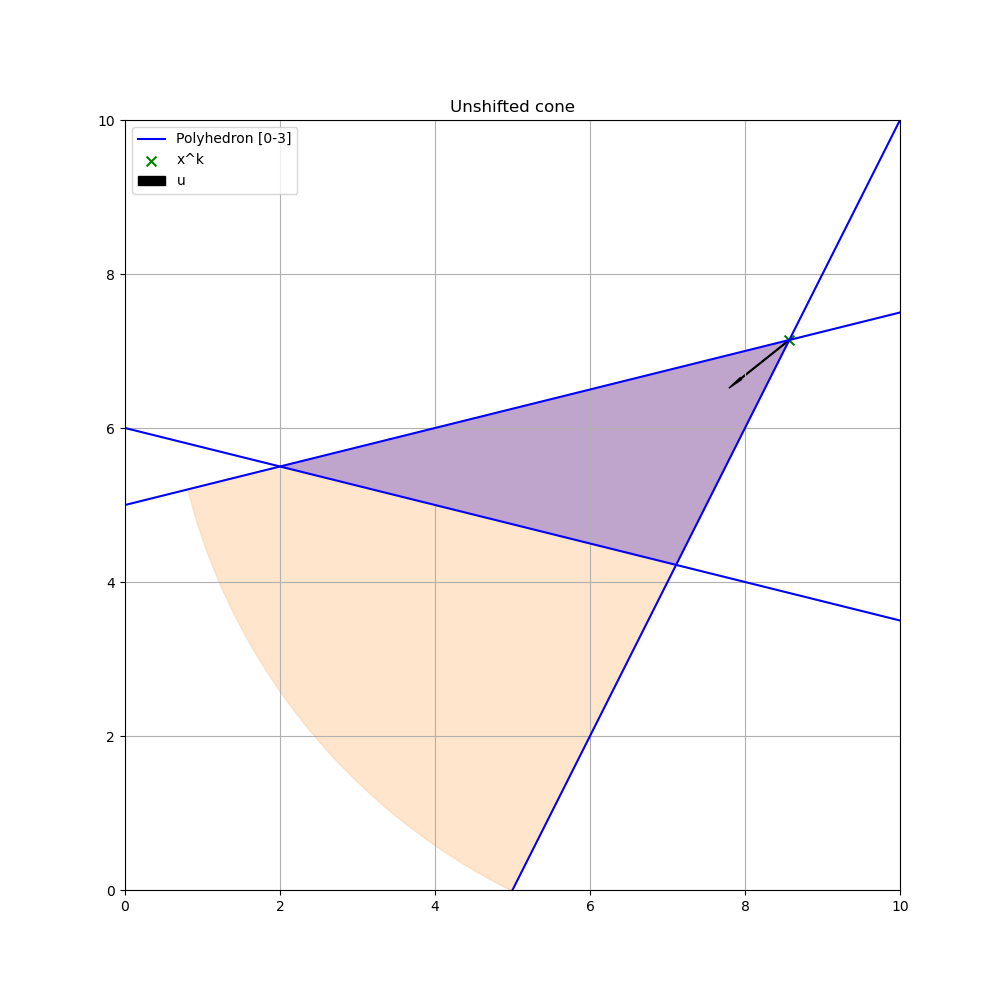
\includegraphics[width=200px]{images/unshifted_cone.png}
%    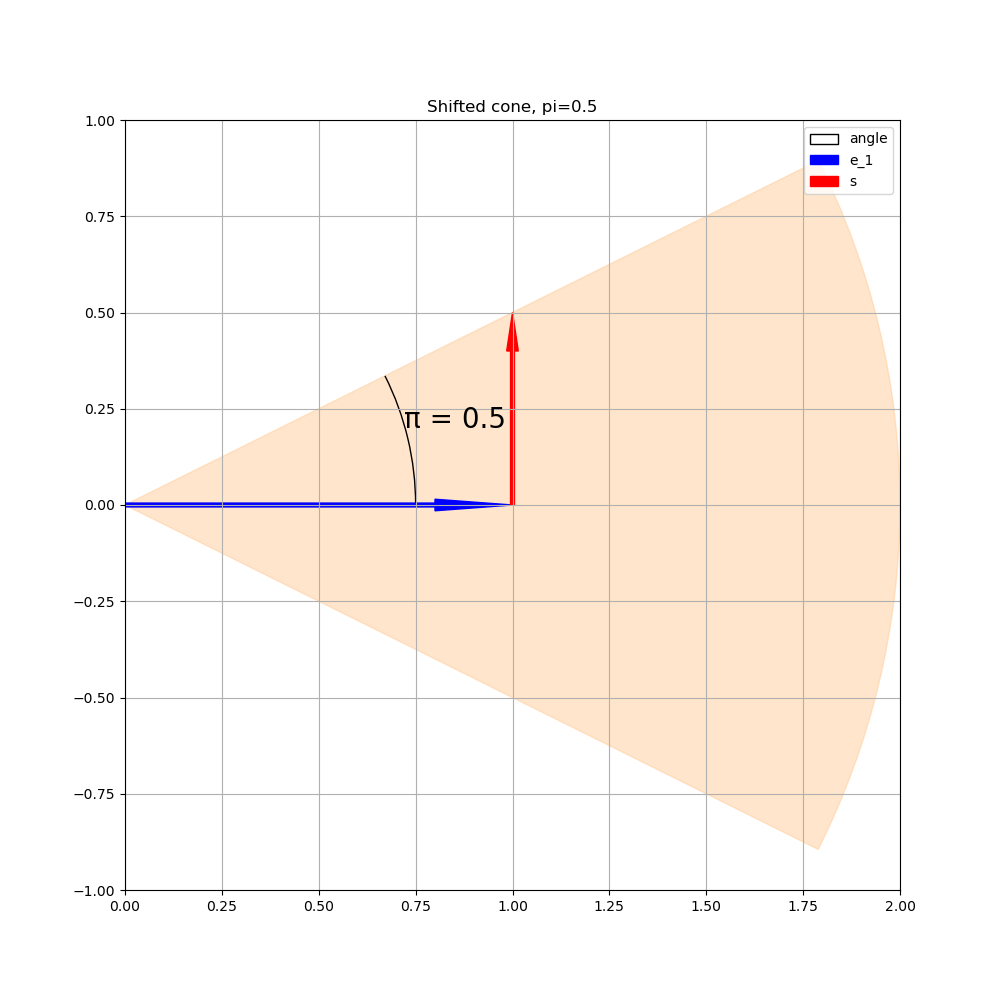
\includegraphics[width=200px]{images/shifted_cone.png}
%    \caption[An example of the shifted and unshifted cones]
%	{   \label{cones}
%		On the left is an unshifted cone $\unshiftedcone$.
%		The zeros of the polyhedron constraint functions are in blue, and the current iterate is in green.
%		A feasible direction $u$ from the current iterate is calculated, and the width of the cone is determined to lie within the active constraints of the polyhedra.
%		On the right is a shifted cone $\unshiftedcone$.
%		It is centered at the origin, and points along $\eone$, opening at a rate of $\alphak$.
%    }
%    \label{linear_cones_images}
%\end{figure}
%
%% \begin{boxedcomment}
%% Illustrate the open rate...
%% \end{boxedcomment}
%
%We first show that  $\unshiftedcone$ is feasible with respect to the active constraints.
%That is, $\lca_i x \le \lcb_i$ for all $x \in \unshiftedcone$ and $i \in \activei\left(\xk\right)$.
%\cref{linear_cones_images} contains a depiction of these cones.
%
%
%% = \left\{x \in \Rn \bigg | \quad x = \xk + t \uk+ s, s^Tu^{\star} = 0, t \ge 0, \|s\| \le {\alphak} t\right\}  \\
%% \left\{x = (t, s)^T \in \Rn, t \in \mathbb R_{\ge 0}, s \in \mathbb R^{n-1} \bigg |\quad \|s\| \le {\alphak} t \right\} 
%
%\begin{lemma}
%\label[lemma]{unshiftedconeisfeasible}
%
%Let $\unshiftedcone$ and $\polyk$ be defined by \cref{defineunshiftedcone} and \cref{polyhedron_k}.
%
%The set $\unshiftedcone$ is feasible with respect to the active constraints of $\polyk$ at $\xk$.  \sbnote{None of the trust region constraints are active at $\xk$, so the active constraints of $\polyk$ are the same as the active constraints of $\feasible$}.
%\end{lemma}
%
%\begin{proof}
%
%Note that the trust region boundary cannot be active at $\xk$ as $\dk > 0$.
%Let $\activei$, $\alphak$, and $\uk$ be defined by \cref{define_activei}, \cref{define_alpha_k}, \cref{define_u_k} and
%$\lca$ and $\lcb$ be defined by \cref{eq:DFO-linear}.
%Let $y = \xk + t\uk + s \in \unshiftedcone$ and $i \in \activei\left(\xk\right)$ be arbitrary.
%Then,
%\begin{align*}
%{\lca}_{i}^Ty - {\lcb}_{i} = {\lca}_{i}^T(t\uk + s) = {\lca}_{i}^Ts + t {\lca}_{i}^T\uk \le \|s\| - \alphak t \le 0.
%\end{align*}
%\end{proof}
%
%The following function is useful for showing results about our ellipsoids:
%\begin{align}
%f_{e}(\pi, \delta, r; x) = (x - \delta \eone)^T
%\begin{pmatrix}
%1 & \boldsymbol0^T \\
%\boldsymbol 0 & \pi^{-2} \boldsymbol I \\
%\end{pmatrix}
%(x - \delta \eone) - r. \label{define_ellipsoid_function}
%\end{align}
%
%%\begin{lemma}
%%
%%\label[lemma]{shifted_ellipsoid_in_cone}
%%For any $\itbound \in (0, 2]$, let $\shiftedcone, f_e, \alphak$ be defined as in \cref{defineshiftedcone}, \cref{define_ellipsoid_function}, \cref{define_alpha_k}.
%%Then, for all $\delta > 0$, the ellipsoid
%%\begin{align}
%%\left\{x \in \Rn \bigg | f_e\left(\alphak, \delta, \frac {\delta^2}{\itbound^2}; x\right) \le 0 \right\} \subseteq \shiftedcone.
%%\end{align}
%%\end{lemma}
%%
%%\begin{proof}
%%
%%Suppose that $x \in \left\{x \in \Rn \bigg| f_e\left(\alphak, \delta, \frac {\delta^2}{\itbound^2}; x\right) \le 0 \right\}$,
%%and let $t = x^T\eone$, $s=x - t \eone$. 
%%Then $f_e(x) \le 0$ implies
%%\begin{align*}
%%\frac {\delta^2}{\itbound^2} \ge \frac {\delta^2}{2}&\ge
%%(x - \delta \eone)^T\begin{pmatrix}
%%1 & \boldsymbol0^T \\
%%\boldsymbol 0 & \left(\alphak\right)^{-2} \boldsymbol I \\
%%\end{pmatrix}(x - \delta \eone)  \\
%%& = (t - \delta)^2 + \frac {1} {\left(\alphak\right)^2} \|s\|^2 \\
%%\Longrightarrow \|s\|^2 &\le \left(\alphak\right)^2 \left[\frac {\delta^2}{2} - (t - \delta)^2\right] \\
%%&= \left(\alphak\right)^2 \left[t^2 - 2\left(t - \frac {\delta}{\itbound}\right)^2 \right] \le \left(\alphak\right)^2t^2 \\
%%\Longrightarrow \|s\| &\le \alphak t. \\
%%\end{align*}
%%Thus, $x \in\shiftedcone$.
%%\end{proof}
%
%
%
%\begin{lemma}
%\label[lemma]{linear_mapping_works}
%
%Let $\rotk$, $T_k$, $\unshiftedcone$, $\shiftedcone$ be defined as in
%\cref{define_r}, \cref{define_affine_mapping}, \cref{defineunshiftedcone}, \cref{defineshiftedcone}.
%Then $T_k\left(\unshiftedcone\right) = \shiftedcone$.
%% and $T_k^{-1}(\shiftedcone) = \unshiftedcone$
%\end{lemma}
%
%\begin{proof}
%
%Observe that $\rotk \eone = \uk$, $\rotk \uk = \eone$, $\det(\rotk) = 1$, and 
%$\rotk \rotk ^T = \rotk ^T\rotk = I$.
%
%Suppose that $x \in \unshiftedcone$.
%Then there exists $t \ge 0$ and $s \in \Rn$ such that $x = \xk + t \uk+ s$ where $s^T \uk = 0$ and $\|s\| \le {\alphak} t$.
%Then $T_k(x) = t\rotk\uk + \rotk s = t\eone + \rotk s$.
%Observe that $(Rs)_1 = (\rotk s)^T\eone = s^T\rotk^T(\rotk \uk) = s^T \uk = 0$.
%Hence,
%$T_k(x) = \begin{pmatrix}
%t \\
%\sigma
%\end{pmatrix}$ where $\sigma \in \mathbb R ^ {n-1}$ satisfies $\|\sigma\| = \|s\| \le \alphak t$.
%Thus, $T_k(x) \in \shiftedcone$.
%Conversely, if $\begin{pmatrix}
%t \\
%\sigma
%\end{pmatrix} \in \shiftedcone$, then let
%$s = \rotk^T\begin{pmatrix}
%0 \\
%\sigma
%\end{pmatrix}$
%to see that
%$x = T_k^{-1}\left(\begin{pmatrix}
%t \\
%\sigma
%\end{pmatrix} \right)= \rotk^T\left(t \eone + \begin{pmatrix}
%0 \\
%\sigma
%\end{pmatrix}\right) = t \uk + s$, where
%$\|s\| = \|\sigma\| \le \alphak t$.
%Hence $T_k^{-1}\left(\begin{pmatrix}
%t \\
%\sigma
%\end{pmatrix}\right) \in \unshiftedcone$.
%\end{proof}
%
%
%\begin{lemma}
%\label[lemma]{ellipsoid_fits}
%
%Let $\activei$, $f_e$, $\deltaf$ $\alphak$, $\rotk$, $T_k$, and $\polyk$ be defined by
%\cref{define_activei}, \cref{define_ellipsoid_function}, \cref{define_deltaf}, \cref{define_alpha_k}, \cref{define_r}, \cref{defineshiftedcone}, and \cref{polyhedron_k},
%respectively.
%
%For each iteration $k$, if $\activei\left(\xk\right) \ne \emptyset$, the ellipsoid
%\begin{align}
%\ellipsek = \left\{x \in \Rn \bigg | f_e\left(\alphak, \deltaf, \frac {\deltaf^2} {\itbound^2}; T_k(x)\right) \le 0\right\} \label{definefeasibleellipsoid}
%\end{align}
%satisfies $\ellipsek \subset \polyk$.
%\end{lemma}
%
%\begin{proof}
%
%
%
%Let $\alphakp$, $\rotk$, $\unshiftedcone$, $\dnearcons\left(\xk\right)$, and $\shiftedcone$ be defined by
%\cref{define_alphakp}, \cref{define_r}, \cref{defineunshiftedcone}, \cref{nearestnonactive}, and \cref{defineshiftedcone},
%respectively.
%We see that if $x \in \ellipsek$,
%then by \cref{shifted_ellipsoid_in_cone} we have that $T_k(x) = \begin{pmatrix}t\\ \sigma\end{pmatrix} \in \shiftedcone$ for some $\sigma \in \mathbb R^{n-1}$
%with $\left\|\sigma\right\| \le \alphak$, and
%\begin{align*}
%\frac {\deltaf^2}{\itbound} \ge
%(x - \deltaf \eone)^T\begin{pmatrix}
%1 & \boldsymbol0^T \\
%\boldsymbol 0 & \left(\alphak\right)^{-2} \boldsymbol I \\
%\end{pmatrix}(x - \deltaf \eone)
% = \left(t - \deltaf\right)^2 + \frac {1} {\left(\alphak\right)^2}\left\|\sigma\right\|^2
%\ge (t - \deltaf)^2  \\
%\Longrightarrow t \le \left(1 + \itbound^{-1}\right)\deltaf
%\end{align*}
%\color{magenta}
%\begin{align*}
%\frac {\deltaf^2} {\itbound^2} \ge (t - \deltaf)^2
%\Longleftrightarrow \deltaf \ge \itbound (t - \deltaf)
%\Longleftrightarrow \frac 1 {\itbound} \deltaf \ge  t - \deltaf
%\Longleftrightarrow \left(1 + \itbound^{-1}\right) \deltaf \ge  t
%\end{align*}
%\color{black}
%so that 
%\begin{align*}
%\|x\|^2 = t^2 + \|\sigma\|^2 \le t^2 + \left(\alphak\right)^2 t^2
%\le \left[1 + \left(\alphak\right)^2 \right] \left(1 + \itbound^{-1}\right)^2\deltaf^2
%= \left(\alphakp\right)^2 \deltaf^2 \\
%\Longrightarrow \|x\| \le \alphakp \deltaf \le \dnearcons\left(\xk\right).
%\end{align*}
%Thus, all points within $\ellipsek$ are closer than the nearest point of a non-active constraint.
%Combine this with \cref{unshiftedconeisfeasible} to see that $\ellipsek \subset \polyk$.
%\end{proof}
%
%
%
%\begin{lemma}
%\label[lemma]{ellipsoid_includes_origin}
%
%For any constant $\itbound > 1$, and any iteration $k$,
%let $f_e$, $\deltaf$, $\rotk$, $T_k$, $\unshiftedcone$, $\shiftedcone$, $\polyk$ be defined as in
%\cref{define_ellipsoid_function}, \cref{define_deltaf}, \cref{define_r}, \cref{define_affine_mapping}, \cref{defineunshiftedcone}, \cref{defineshiftedcone}, \cref{polyhedron_k}.
%
%Then the ellipsoid
%\begin{align}
%\scaledellipsek  = \left\{x \in \Rn \bigg | f_e\left({\alphak}, \deltaf, \deltaf^2; T_k(x)\right) \le 0\right\} \label{definescaledfeasibleellipsoid}
%\end{align}
%satisfies $\xk \in \itbound \sampletrk$.
%\end{lemma}
%
%\begin{proof}
%
%We have that
%\begin{align*}
%f_e\left(\alphak, \deltaf, \deltaf^2; T_k\left(\xk\right) \right)
%&=
%f_e\left({\alphak}, \deltaf, \deltaf^2; 0\right) \\
%&=
%(0 - \deltaf \eone)^T\begin{pmatrix}
%1 & \boldsymbol0^T \\
%\boldsymbol 0 & \left(\alphak\right)^{-2} \boldsymbol I \\
%\end{pmatrix}(0 - \deltaf \eone) - \deltaf^2 \\
%&= \deltaf^2 - \deltaf^2 = 0.
%\end{align*}
%\end{proof}
%
%
%
%\begin{lemma}
%\label[lemma]{nontrivial_ellipsoid_exists}
%
%Let $\activei$ and ${\alphak}$ be defined by \cref{define_activei} and \cref{define_alpha_k}, respectively.
%
%Suppose that \cref{interior_point} holds.
%
%For some iteration $k$, if $\activei \ne \emptyset$, then the ellipsoid defined by \cref{define_linear_nontrival_ellipsoid}
%is suitable according to \cref{define_suitable_ellipsoid}.
%
%% For iteration $k$, if ${\alphak} > 0$, then there exists a suitable ellipsoid for iteration $k$ according to .
%\end{lemma}
%
%\begin{proof}
%
%\color{magenta}
%For $\delta \in \left\{1, \itbound^2\right\}$:
%\begin{align*}
%\left(x - \ck\right)^T\qk\left(x - \ck\right) \le \delta \\
%\Longleftrightarrow
%\left(x - \xk+\deltaf \uk \right)^T\frac {\itbound^2} {\delta_f^2} \rotk^T \begin{pmatrix}
%1 & \boldsymbol0^T \\
%\boldsymbol 0 & \left({\alphak}\right)^{-2} \boldsymbol I \\
%\end{pmatrix} \rotk\left(x - \xk+\deltaf \uk \right) \le \delta \\
%\Longleftrightarrow
%\left[\rotk\left(x - \xk\right)+\deltaf \rotk \uk \right]^T \begin{pmatrix}
%1 & \boldsymbol0^T \\
%\boldsymbol 0 & \left({\alphak}\right)^{-2} \boldsymbol I \\
%\end{pmatrix} \left[\rotk\left(x - \xk\right)+\deltaf \rotk \uk \right] \le \frac 1 {\itbound^2} \delta\delta_f^2 \\
%\Longleftrightarrow
%\left(T_k(x) + \deltaf \eone \right)^T \begin{pmatrix}
%1 & \boldsymbol0^T \\
%\boldsymbol 0 & \left({\alphak}\right)^{-2} \boldsymbol I \\
%\end{pmatrix} \left(T_k(x) + \deltaf \eone \right) - \frac 1 {\itbound^2} \delta\delta_f^2 \le 0\\
%\left[
%\Longleftrightarrow (x - \delta \eone)^T
%\begin{pmatrix}
%1 & \boldsymbol0^T \\
%\boldsymbol 0 & \pi^{-2} \boldsymbol I \\
%\end{pmatrix}
%(x - \delta \eone) - r \le 0 \right]\\
%\Longleftrightarrow f_{e}(\alphak, \deltaf,\frac 1 {\itbound^2} \delta\delta_f^2; T_k(x)) \le 1
%\end{align*}
%
%\color{black}
%
%Let 
%$f_e$,
%$T_k$,
%$\rotk$, $\deltaf$, and $\scaledunshiftedellipsoid$
%be defined as in
%\cref{define_ellipsoid_function},
%\cref{define_affine_mapping},
%\cref{define_r},
%\cref{definefeasibleellipsoid}, and
%\cref{definescaledfeasibleellipsoid},
%respectively. 
%Observe that \cref{define_suitable_ellipsoid} with \cref{define_linear_nontrival_ellipsoid} defines  $\ellipsek$ and $\scaledellipsek$ to be
%\begin{align*}
%\begin{array}{cccc}
%\ellipsek &=& \left\{x \in \Rn \bigg | f_e\left(\alphak, \deltaf, \frac {\deltaf^2} {\itbound^2} ; T_k(x)\right) \le 0\right\}, &\quad \textrm{and}  \\
%\scaledellipsek &=& \left\{x \in \Rn \bigg | f_e\left({\alphak}, \deltaf, \deltaf^2; T_k(x)\right) \le 0\right\}.&
%\end{array}
%\end{align*}
%
%By \cref{ellipsoid_fits}, we know that $\ellipsek \subset \polyk$.
%By \cref{ellipsoid_includes_origin}, we know that $\xk \in \itbound \sampletrk$ .
%By \cref{alphas_are_bounded}, there exists $\epsilon_{\alpha} > 0$, such that the condition number 
%$\condition\left(\qk\right) = \frac{\max\{1, {\alphak}^{-2}\}}{\min\{1, {\alphak}^{-2}\}} = \left({\alphak}\right)^{-2} > 0$.
%This is because $\det\left(\rotk\right) = 1$ means the condition number of $\qk$ is not affected $\rotk$.
%\end{proof}


\section{Results}

% Here, we present numerical results for our implementations of \cref{linearly_constrained_dfo_simple}.

\subsection{Hock-Schittkowksi test problems}


We tested these algorithms on several problems from the Hock-Schittkowski problem set \cite{Schittkowski1981MoreTE} and \cite{Hock1980}.
We selected the problems that have linear constraints: 21, 24, 25, 35, 36, 44, 45, 76, 224, 231, 232, 250, 251.
We summarize the results within \color{magenta} a section to come \color{black}.

% 37 was left out because it proved to be difficult.

\paragraph*{Performance profile.}
\label{performance_profile}
In order to better evaluate the algorithms on the problems across in this test set, we use a performance profile developed in \cite{More:2009:BDO:1654367.1654371}.
Given a set of Solvers $\mathcal S$ that solved a set of problems $\mathcal P$ with the number of evaluations of solver $s$ on problem $p$ being $N(s, p)$, the performance ratio is defined to be $r(s, p) = \frac{N(s, p)}{\min_{s \in \mathcal S} N(s, p)}$.
If the algorithm does not complete, then the number of evaluations is set to $\infty$.
The performance profile of a solver $s$ and parameter $\alpha \in [0, \infty)$ is then the number of problems for which the performance ratio is less than or equal to $\alpha$: 

\begin{align}
\rho(s, \alpha) = \frac 1 {\left\|\mathcal P \right\|} \left\|p \in \mathcal P | r(s, p) \le \alpha\right\|.
\end{align}

The $y$ axis of a performance plot is the performance profile, and the $x$ axis is the parameter $\alpha$.
Note that algorithms with high performance profiles for small values of $\alpha$ solved a large number of problems the most with the fewest evaluations, while algorithms that eventually reach high performance profiles with larger values of $\alpha$ solve a large set of problems.
The performance profile for the Hock-Schittkowski problem set is given in figure \cref{performance_profile_image}.

	
\begin{figure}[ht]
    \centering
    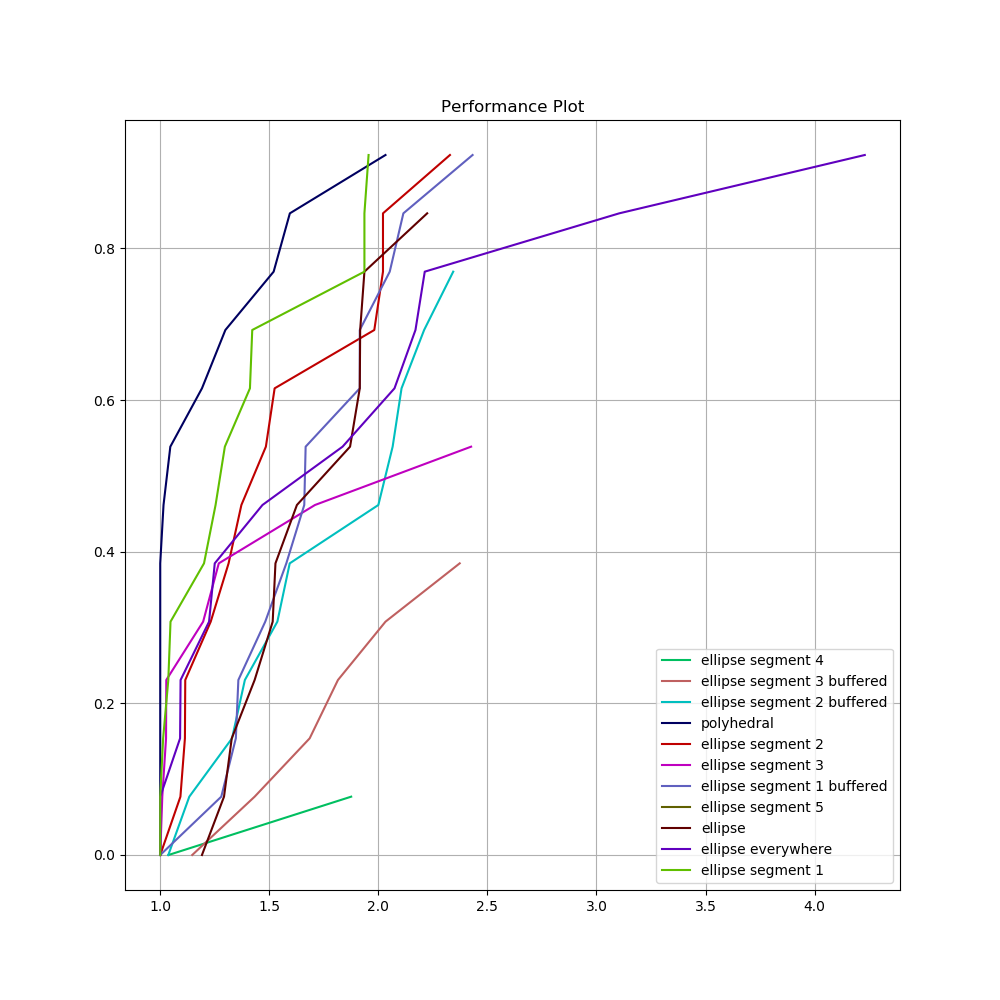
\includegraphics[scale=0.4]{images/performance_profile_plot.png}
    \caption[A performance profile comparing variants of the algorithm for linear constraints.]{
    	A performance profile comparing different variants of the algorithm for linear constraints.
    	We see that the polyhedral algorithm is both efficient and robust.
    }
    \label{performance_profile_image}
\end{figure}

\section{TO DO}
\begin{enumerate}
\item Literature review
\item \cref{replacing_h3} requires the sample points to be lambda poised.
\item Should we remove the first bullet point of Theorem 3.12 on page 15.
\item We could provide the rules for trust region radius updates before the algorithm in the given section.
\item I can superscript each of the V's in the eigen decomposition based in the iteration k.
\end{enumerate}



\bibliography{thesis}
\bibliographystyle{ieeetr}
\end{document}
